\documentclass[10pt,b5paper,twoside,openright]{book}
%Template for project and MSc project reports created by MSc Morten Fyhn Amundsen
\usepackage{graphicx}
\graphicspath{ {report/figures} }
\usepackage{config}


% err math function
\DeclareMathOperator\err{err}
\DeclareMathOperator\std{std}
\DeclareMathOperator\abs{abs}
\DeclareMathOperator\mean{mean}
% \DeclareMathOperator\min{min}
\DeclareMathOperator\outliers{outliers}
\DeclareMathOperator\inliers{inliers}
\DeclareMathOperator\score{score}
\usepackage{mathtools,xparse}
\DeclarePairedDelimiter{\norm}{\lVert}{\rVert}


\usepackage{caption}
\usepackage{amsmath}
\usepackage[space]{grffile}
\usepackage[colorinlistoftodos]{todonotes}
%getting bold symbols in math mode
\usepackage{bm}


% \usepackage[toc,nopostdot,nonumberlist,style=super,acronym]{glossaries}
% \makeglossaries
% \renewcommand*{\acronymname}{List of Abbreviations}
\usepackage{booktabs}





 

\usepackage[section]{placeins}
\makeatletter
\AtBeginDocument{%
  \expandafter\renewcommand\expandafter\subsection\expandafter{%
    \expandafter\@fb@secFB\subsection
  }%
}
\makeatother
\makeatletter
\AtBeginDocument{%
  \expandafter\renewcommand\expandafter\section\expandafter{%
    \expandafter\@fb@secFB\section
  }%
}
\makeatother

%citing: write all articles in the .bib file. Only the ones that are cited in the project will appear
% in the bibliography
% \usepackage{biblatex}
% \addbibresource{master.bib}




\begin{document}


\frontmatter
\pagestyle{plain}
\begingroup
\let\cleardoublepage\clearpage
%Problem description - describing the project tasks, supervisor and co-supervisor - is the first page of the report. For MSc theses this is generated by the DAIM system. For project reports, you generate this page yourself.
\chapter*{Preface}
\addcontentsline{toc}{chapter}{Preface}

    
    This thesis has four listed supervisors for this thesis. Lars Imsland has been my main supervisor, we have met almost every other week during the thesis. Lars has been available for discussions about the case and methods used in this thesis. Anders Willersrud has been my co-supervisor from Hymatek Controls. Anders has been available for discussion during the thesis as well. Mostly through Skype, but I was at one occasion in Oslo at Hymatek to discuss the different possible cases I had found in the dataset. Beatriz Galindo-Prieto and Frank Westad were brought on-board as co-supervisors to help with missing data in dataset. Both Beatriz and Frank looked at the data to try to solve the problem with missing data, in addition we discussed possible techniques for feature selection from a larger dataset. Unfortunately no good solutions were found to the missing data problem, and my work with Frank and Beatriz did not result in any contribution to the thesis.
    
    During this thesis I have been working on a dataset from 27 Hydroelectric power plants provided by Hymatek. In addition they provided a log of recorded incidents and maintenance at the plants. I have been working on a Dell desktop provided by NTNU in Ubuntu, using the Anaconda distribution to manage my Python environment. Keras and Scikit-learn have been used as machine learning libraries. In my project thesis I looked into the possibility to classify the condition of the guide vanes of a Francis turbine. The code used for one class support vector machines is reused from my project thesis. The rest of the framework used in this thesis, has been written by me during the master thesis. This includes a library for reading and converting the dataset provided by Hymatek into a form that could be analyzed. 
    
    In this thesis three different anomaly detection techniques are tested on Pelton turbines. One class support vector machine was used in my project thesis. The two others are proposed by myself after searching the literature. I found the Pelton case when looking through the data and plant logs provided by Hymatek. It was chosen as a good use-case in cooperation with Hymatek and Lars. No literature has been provided, and all papers and articles used in this thesis are a result of my own literary research.

    I want to thank all my supervisors for their help during my thesis, and Hymatek for providing such an extensive data set. 
    
    \begin{center}
    Trondheim, \today, \\
    % \vspace{1.5cm}
    Asgeir Øen Åsnes
    \end{center}

    % For at sensorene skal få et klarest mulig inntrykk av bidraget fra kandidaten må dette gå klart fram av masteroppgaven.
    % Studenten må derfor beskrive følgende i forordet til masteroppgaven:
    %     Hvilken informasjon, programvare, utstyr osv. som er stilt til rådighet eller danner basis for arbeidet
    %     Hvilken hjelp som er mottatt og fra hvem underveis
    % Faglærer deltar ikke i sensuren, men må attestere at informasjonen i forordet er riktig
    %     Send derfor forordet til faglærer i god tid før innlevering så dere blir enige om beskrivelsen
    % Innleveringsskjema må leveres umiddelbart etter innlevering av masteroppgaven. Dette er en forutsetning for start av sensur

%!TEX root = ../Thesis.tex
\chapter*{\englishabstractname}
\addcontentsline{toc}{chapter}{\englishabstractname}

Much research can be found on condition monitoring for many industries. There are, however, very little research on the use of condition monitoring in hydroelectric power plants. Most of the existing research involves methods that require both normal and abnormal data, and need data for all failure modes that one want to monitor. A literature study investigates this field, and it is found that support vector machines and neural networks have been successfully used for condition monitoring of known failure modes. 

Anomaly detection is presented as it enables the detection of anomalies in the process data, with only normal process data available. Three different methods for anomaly detection are presented, support vector machines, kernel density estimation and long short term neural networks. In addition, different techniques for feature and dimensionality reduction are presented. A data set containing data from 27 power plants is analyzed, and a reported incident with operational problems for the needles of a Pelton turbine is extracted for analysis. Data from two different plants and three different turbines are included in the analysis to investigate cross plant performance. An artificial error replicating the operational problems for the reported incident is created to verify how early the anomaly detection techniques can detect system degradation. In addition, two Pelton turbine start failures are included in the analysis to verify that the methods correctly detect abnormal system data. 

All three methods are shown able to detect the operational problems for the Pelton needles. However, the one class support vector machine is shown to very dependent on the choice of hyperparameters with regards to the training data. Kernel density estimation and long short term recurrent neural network show better performance and are more robust with regards to parameterization and training data. It is also shown that they can detect the early signs of the system degradation seen leading up to the reported incident with the Pelton needles. 

\clearpage

%!TEX root = ../Thesis.tex
\chapter*{\norwegianabstractname}
\addcontentsline{toc}{chapter}{\norwegianabstractname}
%
Sammendraget skal gi en kort oppsummering av innholdet i rapporten.
%
\clearpage

\tableofcontents \clearpage
\section*{{\Huge Abbreviations}}
\addcontentsline{toc}{chapter}{Abbreviations}
$\\[0.5cm]$

\noindent 
\begin{center}
\begin{tabular}{ l c l }
   MI & = &Mutual Information \\
   SVM & = &Support Vector Machine \\
   OC SVM & = & One class Support Vector Machine \\
   NN & = & Neural network \\
   RNN & = & Recurrent neural network\\
   LSTM RNN & = &Long Short Term Recurrent Neural Network \\
   PDF & = & Probability Density Function \\
   RBF & = & Radial Basis Function \\
   PCA & = & Principal Component Analysis \\
   KDE & = & Kernel Density Estimation \\
   SVD & = & Singular value decomposition\\
%   CM & = & Condition Monitoring \\
\end{tabular}
\end{center}

\cleardoublepage

% \pagestyle{fancy}
% \fancyhf{}
% \renewcommand{\chaptermark}[1]{\markboth{\chaptername\ \thechapter.\ #1}{}}
% \renewcommand{\sectionmark}[1]{\markright{\thesection\ #1}}
% \renewcommand{\headrulewidth}{0.1ex}
% \renewcommand{\footrulewidth}{0.1ex}
% \fancyfoot[LE,RO]{\thepage}
% \fancyhead[LE]{\leftmark}
% \fancyhead[RO]{\rightmark}
% \fancypagestyle{plain}{\fancyhf{}\fancyfoot[LE,RO]{\thepage}\renewcommand{\headrulewidth}{0ex}}

\pagenumbering{arabic} 				
\setcounter{page}{1}

% import the list


%List of Acronyms, and List of symbols can be useful to include if you have many.
\endgroup

\mainmatter
\pagestyle{headings}
%!TEX root = ../Thesis.tex
\chapter{Introduction}\label{cha:introduction}
%
% This introductory chapter will briefly provide context for the material/results presented in this report and give motivation and a description of the problem to be solved. A literature review summarizes existing relevant knowledge and establishes the foundation of the later control system. The scope of the work is then defined by a list of assumptions. Finally, the contributions of the thesis are defined and elaborated.

This is a master thesis written in cooperation between NTNU and Hymatek Controls. Hymatek Controls is located in Oslo and delivers equipment and control systems to hydroelectric power plants worldwide. Hymatek is increasing its focus on condition monitoring and anomaly detection, and has acquired a large dataset containing data from a five year period for $27$ hydroelectric power-plants. The goal of this thesis is to find possible use cases for condition monitoring in the provided dataset, research possible techniques and implement some of them in the found use case. Since this is a new research area for Hymatek, this thesis will cover a wide range of aspects. 

This chapter provides an introduction to the work done, describing the motivation and problem description for the thesis. In addition, a literature review looking into state of the art techniques used for condition monitoring. Finally, the outline of the report is presented. 


\section{Motivation}\label{sec:motivation}

% % What is the motivation for considering the problems/question that you approach in your work? Why is this an interesting problem? The motivation should instead describe why it is interesting from a societal point of view, and/or from a scientific point of view.

The need for renewable and stable energy sources is great in Norway, Europe and worldwide. According to \cite{Statkraft2009} $99\%$ of the Norwegian power production comes from hydroelectric power plants. Almost $50\%$ of Europe's hydroelectric capacity is located in Norway. Hydroelectric power is seen as one of the most stable and cleanest energy sources one can find \cite{Statkraft2009}. Hydroelectric power plants have a high investment cost, but according to \cite{Selak2014} operation and maintenance costs are as low as 2\% of the cost of the initial investment, this makes it one of the cheapest energy sources one can find. As many European countries are transitioning into renewable energy sources, the need for stable and controllable power sources grows. Both wind and solar power production are dependent on weather conditions, and their production capacity can change quickly and unexpectedly. Norway has been called Europe's renewable battery due to its hydroelectric capacity, and the power delivery capacity is growing. By 2021 Norway and Great Britain will be connected through a new underwater power cable. This is an example that shows that Norway is becoming a part of a more complex energy market. As the exporting capacity grows, green energy from Norway can be supplied to reduce the consumption of fossil energy from for example coal from the European continent. This means that increased productivity and efficiency in hydroelectric power plants effectively can help make the green shift in the European power production happen. 

One way to increase a plant's productivity, is to ensure that it is operable at all times. This is however not possible since one has to perform maintenance on all parts of a plant. Planned maintenance is however not the only reason for a power plant stopping down. Components can breakdown outside of their service interval, leading to unplanned downtime. This is of course not only a case for hydroelectric power plants but for more or less any industry or factory. Unplanned downtime is expensive for the energy company that operates the plant, and depending on the time of year and the duration of the breakdown, the cost can have a large impact on their operation. Finding a way to avoid these breakdowns, and replacing unplanned maintenance with planned maintenance, is something all energy companies are interested in. A hydroelectric power plant contains several large components such as turbines, generators, transformers, hydraulic systems, valves, pipes etc. In addition, you have all the equipment needed to operate the plant. Keeping spare parts for all components would require an enormous storage, in addition to tying large assets due to the cost of all components. In addition, many components don't need to be replaced often, hence the spare can be left in storage for many years, and may even never be replaced. Clearly, this is not an optimal solution. 

Another approach is to try to eradicate unexpected breakdowns. This means that one needs to have a way to detect that a component is decaying so that one can plan an overhaul or replacement before it breaks down. This also solves another factor to consider when it comes to breakdowns of components, the domino effect. Depending on the situation and the component, if one component breaks down, it might end up taking several other with it. If a bearing on a turbine shaft breaks down, one risks that the damage will spread to the bearing on the other side of the shaft, and even to the turbine and generator. A continuous analysis of the condition of the bearing could help avoid this issue. This is known as condition monitoring. In its most complete form, condition monitoring gives an insight into the condition of the monitored components, giving an estimate to the remaining lifetime of the component. Introducing condition monitoring could help reduce the number of breakdowns, as components can be replaced before breaking.

There are many good reasons for pursuing the topic of this thesis, on a personal level it is motivating to work with real-world data, to learn the difference between theoretical and practical engineering. Looking for solutions that will improve the operation of a hydroelectric power plant, which can give even more clean energy is also motivating. Additionally, the fact that possible solutions found for the specific cases looked into most likely can be adapted to other industries is also very motivating. 

% An attempt of classifying the wear of the guide vanes on a Francis turbine was performed in my project thesis.  


% This triggered my interest in the possibilities of information found in data. 
% Looking into different possible techniques for condition monitoring that can be utilized on a real-world dataset will give
% As the world becomes more and more digitized, one can either keep up or be left behind. Condition monitoring is seen as an important part of the future portfolio of Hymatek Controls and a necessary addition to continuing their growth into the future. 

% \section{Contributions}
    


\section{Problem definition}

% Korleis oppsto problemstillinga? dreiv å såg gjennom feiloggen etter interesssante feil. Såg då at det var problemer med nålstryinga for hjartdøla. Starta så å undersøke dataen, og fant etterkvart ut at det er 2 anlegg til som har nålstyring. Dei hadde derimot ikkje raportet feil med nålene, noko som gav meg grunn til å tenke at dei har normal oppførsel. Då kunne eg og starte å samanlikne data mellom kraftverka for å sjå kva som er unormal og normal oppførsel.

No exact problem definition was provided by Hymatek, they provided a dataset containing process-data from $27$ hydroelectric power plants for the period $2013-2017$, and gave no restriction on which plants and cases that could be investigated. A historical incident log was also provided for all plants, with varying level of detail. Based on this, the problem definition was split into three main parts. As this is a thesis built upon an unknown dataset with unknown quality, an important factor is to recognize what the data can be utilized for, and what improvements that could/ need to be done to make the data analysis more extensive. Ideally, the result of the thesis will be a system for condition monitoring for a real-world case found in the dataset. However, since Hymatek is still in the start-up phase of its condition monitoring research, all experiences from this thesis are valuable. Therefore the most important part of the thesis is to understand why or why not one is able to create a condition monitoring system for the given case. Then this thesis can be used as a basis for further condition monitoring case analysis. The three parts are as follows: 

\begin{itemize}
    \item Finding techniques and methods for condition monitoring and anomaly detection. Finding methods for feature extraction and dimensionality reduction to be used in addition with the anomaly detection techniques.
    \item Data preparation and case extraction. The provided data is not ready for analysis, one needs to extract datasets for each of the plants. Once the data is in a format that can be analyzed, the historical data from the plants and the datasets need to be analyzed to build a  case for the further analysis. 
    \item Analyzing the case using the techniques found. Emphasize on how the different techniques perform, and what can/needs to be done to improve the performance. 
\end{itemize}


% \section{Literature review}\label{sec:review}
    

% Start writing about the articles I have already read, can always delete it if it is not relevant in the end. 
%     \subsection{Timeseries forecasting}\label{sec:time_series_forecasting}
    
%     \subsection{One class support vector machine novelty/anomaly detection}\label{sec:ocsvm_novelty_detection}
    
%     \subsection{Neural network novelty/anomaly detection}\label{sec:nn_novelty_detection}
    
%     \subsection{The data set}\label{sec:the_data}
%     The data is provided by Hymatek controls and is collected from more than 30 hydroelectric power plants around Norway, in the period between $01.01.2014$ and $01.07.2017$. 

\section{Limitations}\label{sec:assumptions}
    Since the thesis span over many different research areas, only one case will be analyzed, even if it should be possible to find several more from such an extensive dataset. In addition, only a subset of the suggested techniques will be chosen for analysis, spanning from easy to more complex. There might be algorithms not tested that could be useful for the given case. The techniques are chosen in cooperation with Hymatek. 
    
    Availability of computing power and memory also introduces constraints to the analysis. All analysis is performed on a desktop from dell provided by NTNU. This means that no analysis will be performed using the full datasets, they will be reduced by either feature selection or dimensionality reduction. 
    
    Condition monitoring is a wide field, and creating a full-scale condition monitoring system for one case is too comprehensive. The thesis will, therefore, focus on anomaly/novelty detection for the given case. This means that one will train different techniques on normal operation data, and verify how well the different techniques are able to detect the anomaly found for the specific case. 
    
\section{Hydroelectric power production}\label{ref:sec_hydropower}
    $99\%$ of the Norwegian power production comes from hydroelectric power plants. Hydroelectric power is clean, reliable and once built, it produces cheap energy. \cite{Statkraft2009} claims that no other types of power plants have long expected lifetime and higher efficiency than hydroelectric power. Statkraft also states that countries with the highest increase in energy demand are also countries with the highest unused potential for hydroelectric power. This means that hydroelectric power production can play a big role in the hunt for meeting a global energy demand. There are many old power plants today, so there are also possibilities for modernization and extensions of already existing plants. 
    
    The principal behind hydroelectric power is simple. It utilizes the energy in running water, converting it to electric energy through a turbine. According to \cite{Paish2002}, there are two main types of turbines, impulse and reaction. The difference between the two types is found in how the rotational force is created. The impulse turbine rotor runs in air, and the rotational force is created by a water jet lead onto the turbine blades. The reaction turbine is submerged in water, and the rotational force comes from a lift force created by the oncoming water flow. For the impulse turbine only kinetic energy is used to generate the rotational force, for the reaction both kinetic and pressure energy is used. When the water hits the turbine blades the water pressure is reduced to atmospheric pressure, and all pressure energy is converted to kinetic energy. For the reaction turbine, which is submerged in water, the water pressure is still high, meaning that one need a casing which is sealed from atmospheric pressure. 
    
    % \begin{figure}
    %     \centering
    %     \includegraphics{}
    %     \caption{Principal behind reaction and impulse turbines}
    %     \label{fig:my_label}
    % \end{figure}
    
    
    The two most common turbine types are Francis and Pelton. The type used is mostly defined by the size of the flow and the head of the water. Whether the turbine will be producing power only at optimal flow, or if it will be used for power production over a wider range is also a criterion. 
    
    
    
    \subsection{Pelton turbines}\label{subsec:pelton}
        
        The Pelton turbine is the most common impulse turbine. Water is lead onto to the turbine through a series of needles or valves. The turbine has a set of buckets located on the turbine wheel which splits the water jet in two, where each half is deflected back and falls down into a discharge channel, \cite{Paish2002}. A cross-section of a Pelton turbine is seen in Figure \ref{fig:pelton_turbine}. As one can see the needles are divided equally around the turbine. The amount of produced power is controlled by the number of active needles, and by regulating their opening. Figure \ref{fig:pelton_bucket} shows how the buckets are designed. Where the water jets hit the buckets is easily verifiable by looking at the corroded parts of the buckets. The needles are controlled by a hydraulic system, which is controlled by the power plant control system. To ensure an even momentum on the turbine, all active needles should have the same opening. 
        
        
        \begin{figure}
            \begin{minipage}[b]{0.49\linewidth}
                \centering
                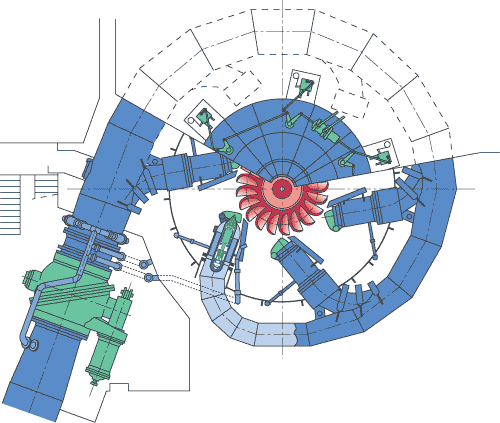
\includegraphics[width = 0.9\textwidth]{report/figures/introduction/pelton.png}
                \caption{Cross section of a Pelton turbine with $6$ needles. By Voith Siemens Hydro Power Generation.\footnote{Licensed under GFDL, Wikimedia Commons \url{https://commons.wikimedia.org/wiki/File:S_vs_pelton_schnitt_1_zoom.png}}} 
                \label{fig:pelton_turbine}
            \end{minipage}
            \hfill\vline\hfill
            \begin{minipage}[b]{0.49\linewidth}
                \centering
                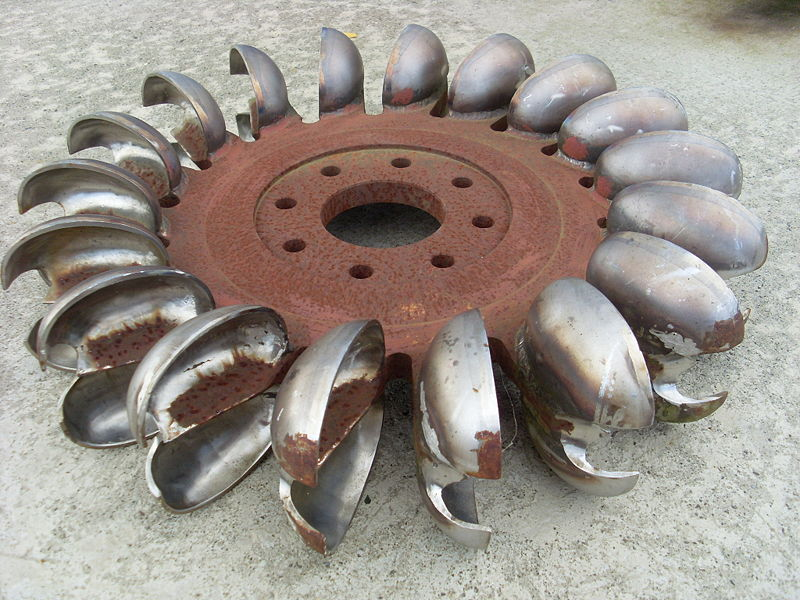
\includegraphics[width = 0.9\textwidth]{report/figures/introduction/pelton_bucket.jpg}
                \caption{A Pelton turbine wheel, the split buckets are easily visible. By Zedh. \footnotetext{Licensed under CC-BY-SA, Wikimedia Commons. \url{https://commons.wikimedia.org/wiki/File:Pelton_400kW_roue_1.JPG}}} 
                \label{fig:pelton_bucket}
            \end{minipage}
        \end{figure}
        
        %!TEX root = ../Thesis.tex
\chapter{Introduction}\label{cha:introduction}
%
% This introductory chapter will briefly provide context for the material/results presented in this report and give motivation and a description of the problem to be solved. A literature review summarizes existing relevant knowledge and establishes the foundation of the later control system. A list of assumptions then defines the scope of the work. Finally, the contributions of the thesis are defined and elaborated.

This is a master thesis written in cooperation between NTNU and Hymatek Controls. Hymatek Controls is located in Oslo and delivers equipment and control systems to hydroelectric power plants worldwide. Hymatek is increasing its focus on condition monitoring and anomaly detection and has acquired a large dataset containing data from a five year period for $27$ hydroelectric power-plants. The goal of this thesis is to find possible use cases for condition monitoring in the provided dataset, research possible techniques and implement some of them in the found use case. Since this is a new research area for Hymatek, this thesis will cover a wide range of aspects. 

This chapter provides an introduction to the work done, describing the motivation and problem description for the thesis. Also, a literature review looking into state of the art techniques used for condition monitoring. Finally, the outline of the report is presented. 


\section{Motivation}\label{sec:motivation}

% % What is the motivation for considering the problems/question that you approach in your work? Why is this an interesting problem? The motivation should instead describe why it is interesting from a societal point of view, and/or from a scientific point of view.

The need for renewable and stable energy sources is great in Norway, Europe and worldwide. According to \cite{Statkraft2009} $99\%$ of the Norwegian power production comes from hydroelectric power plants. Norway has almost $50\%$ of Europe's hydroelectric capacity. Hydroelectric power is one of the most stable and cleanest energy sources one can find \cite{Statkraft2009}. Hydroelectric power plants have a high investment cost, but according to \cite{Selak2014} operation and maintenance costs are as low as 2\% of the cost of the initial investment, this makes it one of the cheapest energy sources one can find. As many European countries are transitioning into renewable energy sources, the need for stable and controllable power sources grows. Both wind and solar power production are dependent on weather conditions, and their production capacity can change quickly and unexpectedly. Norway has been called Europe's renewable battery due to its hydroelectric capacity, and the power delivery capacity is growing. By 2021 Norway and Great Britain will be connected through a new underwater power cable. This example shows that Norway is becoming a part of a more complex energy market. As the exporting capacity grows, green energy from Norway can be supplied to reduce the consumption of fossil energy from for example coal from the European continent. This means that increased productivity and efficiency in hydroelectric power plants effectively can help make the green shift in the European power production happen. 

One way to increase a plant's productivity is to ensure that it is operable at all times. However, this is not possible since one has to perform maintenance on all parts of a plant. Planned maintenance is however not the only reason for a power plant stopping down. Components can breakdown outside of their service interval, leading to unplanned downtime. This is of course not only a case for hydroelectric power plants but more or less any industry or factory. Unplanned downtime is expensive for the energy company that operates the plant, and depending on the time of year and the duration of the breakdown, the cost can have a significant impact on their operation. Finding a way to avoid these breakdowns, and replacing unplanned maintenance with planned maintenance, is something all energy companies find interesting. A hydroelectric power plant contains several large components such as turbines, generators, transformers, hydraulic systems, valves, pipes, and so on.  As an addition comes all the equipment needed to operate the plant. Keeping spare parts for all components would require enormous storage, in addition to tying considerable assets due to the cost of all components. Many components do not need to be often replaced, hence the spare can be left in storage for many years, and may never be replaced. This is not an optimal solution. 

Another approach is to try to eradicate unexpected breakdowns. This means that one needs to have a way to detect that a component is decaying so that one can plan an overhaul or replacement before it breaks down. Eradicating unexpected breakdowns also solves another factor to consider when it comes to breakdowns of components, the domino effect. Depending on the situation and the component, if one component breaks down, it might end up taking several other with it. If a bearing on a turbine shaft breaks down, one risks that the damage will spread to the bearing on the other side of the shaft, and even to the turbine and generator. Continuous analysis of the condition of the bearing could help avoid this issue. This is known as condition monitoring. In its most complete form, condition monitoring gives an insight into the condition of the monitored components, giving an estimate to the remaining lifetime of the component. Introducing condition monitoring could help reduce the number of breakdowns, as components can be replaced before breaking.

There are many good reasons for pursuing the topic of this thesis, on a personal level it is motivating to work with real-world data, to learn the difference between theoretical and practical engineering. Looking for solutions that will improve the operation of a hydroelectric power plant, which can give even more clean energy is also motivating. Additionally, the fact that possible solutions found for the specific cases looked into most likely can be adapted to other industries is also very motivating. 

% An attempt of classifying the wear of the guide vanes on a Francis turbine was performed in my project thesis.  


% This triggered my interest in the possibilities of information found in data. 
% Looking into different possible techniques for condition monitoring that can be utilized on a real-world dataset will give
% As the world becomes more and more digitized, one can either keep up or be left behind. Condition monitoring is seen as an important part of the future portfolio of Hymatek Controls and a necessary addition to continuing their growth into the future. 

% \section{Contributions}
    


\section{Problem definition}

% Korleis oppsto problemstillinga? dreiv å såg gjennom feiloggen etter interesssante feil. Såg då at det var problemer med nålstryinga for hjartdøla. Starta så å undersøke dataen, og fant etterkvart ut at det er 2 anlegg til som har nålstyring. Dei hadde derimot ikkje raportet feil med nålene, noko som gav meg grunn til å tenke at dei har normal oppførsel. Då kunne eg og starte å samanlikne data mellom kraftverka for å sjå kva som er unormal og normal oppførsel.

Hymatek provided no exact problem definition, they provided a dataset containing process-data from $27$ hydroelectric power plants for the period $2013-2017$, and gave no restriction on which plants and cases to investigate. A historical incident log was also provided for all plants, with varying level of detail. Based on this, the problem definition was split into three main parts. As this is a thesis built upon an unknown dataset with unknown quality, an important factor is to recognize what the data can be utilized for, and what improvements that could/ need to be done to make the data analysis more extensive. Ideally, the result of the thesis will be a system for condition monitoring for a real-world case found in the dataset. However, since Hymatek is still in the start-up phase of its condition monitoring research, all experiences from this thesis are valuable. Therefore the most important part of the thesis is to understand why or why not one can create a condition monitoring system for the given case. Then this thesis can be used as a basis for further condition monitoring case analysis. The three parts are as follows: 

\begin{itemize}
    \item Finding techniques and methods for condition monitoring and anomaly detection. Finding methods for feature extraction and dimensionality reduction to be used in addition to the anomaly detection techniques.
    \item Data preparation and case extraction. The provided data is not ready for analysis, and one needs to extract datasets for each of the plants. Once the data is in a format that can be analyzed, the historical data from the plants and the datasets need to be analyzed to build a  case for the further analysis. 
    \item Analyzing the case using the techniques found. Emphasize on how the different techniques perform, and what can/needs to be done to improve the performance. 
\end{itemize}


% \section{Literature review}\label{sec:review}
    

% Start writing about the articles I have already read, can always delete it if it is not relevant in the end. 
%     \subsection{Timeseries forecasting}\label{sec:time_series_forecasting}
    
%     \subsection{One class support vector machine novelty/anomaly detection}\label{sec:ocsvm_novelty_detection}
    
%     \subsection{Neural network novelty/anomaly detection}\label{sec:nn_novelty_detection}
    
%     \subsection{The data set}\label{sec:the_data}
%     The data is provided by Hymatek controls and is collected from more than 30 hydroelectric power plants around Norway, in the period between $01.01.2014$ and $01.07.2017$. 

\section{Limitations}\label{sec:assumptions}
    Since the thesis span over many different research areas, only one case will be analyzed, even if it should be possible to find several more from such an extensive dataset. Also, only a subset of the suggested techniques will be chosen for analysis, spanning from easy to more complex. There might be algorithms not tested that could be useful for the given case. The techniques are chosen in cooperation with Hymatek. 
    
    Availability of computing power and memory also introduces constraints to the analysis. All analysis is performed on a desktop from dell provided by NTNU. This means that no analysis will be performed using the full datasets, they will be reduced by either feature selection or dimensionality reduction. 
    
    Condition monitoring is a broad field, and creating a full-scale condition monitoring system for one case is too comprehensive. The thesis will, therefore, focus on anomaly/novelty detection for the given case. This means that one will train different techniques on normal operation data, and verify how well the different techniques can detect the anomaly found for the specific case. 
    
\section{Hydroelectric power production}\label{ref:sec_hydropower}
    $99\%$ of the Norwegian power production comes from hydroelectric power plants. Hydroelectric power is clean, reliable and once built, it produces cheap energy. \cite{Statkraft2009} claims that no other types of power plants have long expected lifetime and higher efficiency than hydroelectric power. Statkraft also states that countries with the highest increase in energy demand are also countries with the highest unused potential for hydroelectric power. This means that hydroelectric power production can play a significant role in the hunt for meeting the global energy demand. There are many old power plants today, so there are also possibilities for modernization and extensions of already existing plants. 
    
    The principal behind hydroelectric power is simple. It utilizes the energy in running water, converting it to electric energy through a turbine. According to \cite{Paish2002}, there are two main types of turbines, impulse and reaction. The difference between the two types is how they create the rotational force. The impulse turbine rotor runs in air, and the rotational force is created by a water jet lead onto the turbine blades. The reaction turbine is submerged in water, and the rotational force comes from a lift force created by the oncoming water flow. For the impulse turbine, kinetic energy generates the rotational force, for the reaction both kinetic and pressure energy generates it. When the water hits the turbine blades, the water pressure is reduced to atmospheric pressure, and all pressure energy is converted to kinetic energy. For the reaction turbine, which is submerged in water, the water pressure is still high, meaning that one needs a casing which is sealed from atmospheric pressure. 
    
    % \begin{figure}
    %     \centering
    %     \includegraphics{}
    %     \caption{Principal behind reaction and impulse turbines}
    %     \label{fig:my_label}
    % \end{figure}
    
    
    The two most common turbine types are Francis and Pelton. The type used is defined by the size of the flow and the head of the water. Whether the turbine will be producing power only at optimal flow, or if it will be used for power production over a broader range is also a criterion. 
    
    
    
    \subsection{Pelton turbines}\label{subsec:pelton}
        
        The Pelton turbine is the most common impulse turbine. Water is lead onto to the turbine through a series of needles or valves. The turbine has a set of buckets located on the turbine wheel which splits the water jet in two, where each half is deflected back and falls into a discharge channel, \cite{Paish2002}. A cross-section of a Pelton turbine is seen in Figure \ref{fig:pelton_turbine}. As one can see the needles are divided equally around the turbine. The amount of produced power is controlled by the number of active needles, and by regulating their opening. Figure \ref{fig:pelton_bucket} shows how the buckets are designed. Where the water jets hit the buckets is easily verifiable by looking at the corroded parts of the buckets. The needles are controlled by a hydraulic system, which is controlled by the power plant control system. To ensure an even momentum on the turbine, all active needles should have the same opening. 
        
        
        \begin{figure}
            \begin{minipage}[b]{0.49\linewidth}
                \centering
                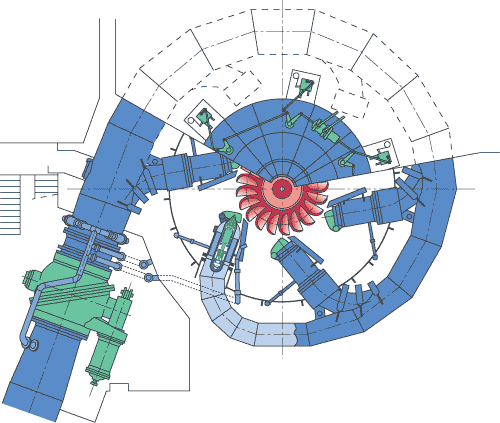
\includegraphics[width = 0.9\textwidth]{report/figures/introduction/pelton.png}
                \caption{Cross section of a Pelton turbine with $6$ needles. By Voith Siemens Hydro Power Generation.\footnote{Licensed under GFDL, Wikimedia Commons \url{https://commons.wikimedia.org/wiki/File:S_vs_pelton_schnitt_1_zoom.png}}} 
                \label{fig:pelton_turbine}
            \end{minipage}
            \hfill\vline\hfill
            \begin{minipage}[b]{0.49\linewidth}
                \centering
                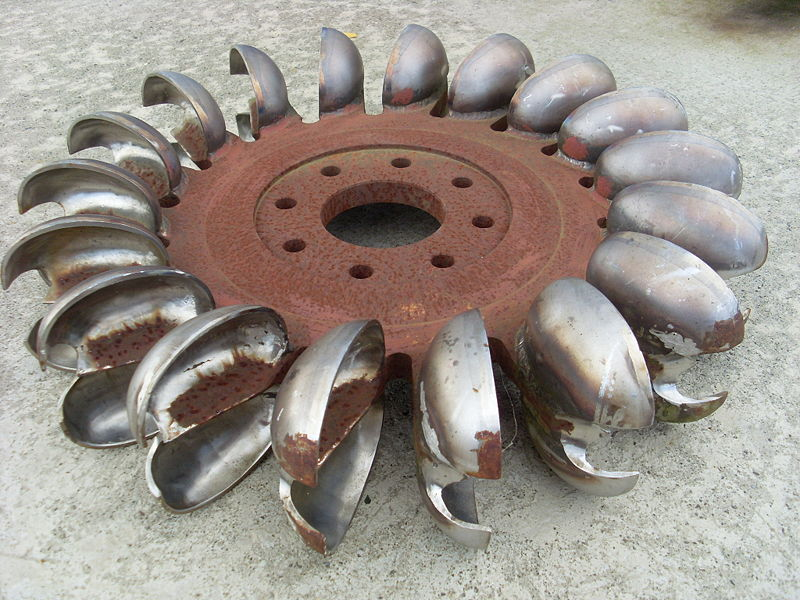
\includegraphics[width = 0.9\textwidth]{report/figures/introduction/pelton_bucket.jpg}
                \caption{A Pelton turbine wheel, the split buckets are easily visible. By Zedh. \footnotetext{Licensed under CC-BY-SA, Wikimedia Commons. \url{https://commons.wikimedia.org/wiki/File:Pelton_400kW_roue_1.JPG}}} 
                \label{fig:pelton_bucket}
            \end{minipage}
        \end{figure}
        
        
    
    \subsection{Francis turbines}\label{subsec:francis}
        The Francis turbine is a reaction turbine. The water is lead onto the turbine through a set of guide vanes connected to the spiral casing, and lead out from the center of the turbine. The guide vanes control the amount of water lead to the turbine, and hence the amount of produced energy. A cross-section of a Francis turbine is seen in Figure \ref{fig:francis}. All guide vanes have the same opening and are controlled through a ring mounted on the top of the turbine. Figure \ref{fig:guide_vanes} shows a hydraulic actuator used to control the ring that operates the guide vanes. As for the Pelton turbine, the hydraulics is again controlled by the plant's control system. \cite{Aasnes2017} tries to classify the condition of the guide vanes in a Francis turbine using different machine learning methods such as support vector machines (SVM), neural networks (NN) and regression.   
        
        \begin{figure}
            \begin{minipage}[b]{0.49\linewidth}
                \centering
                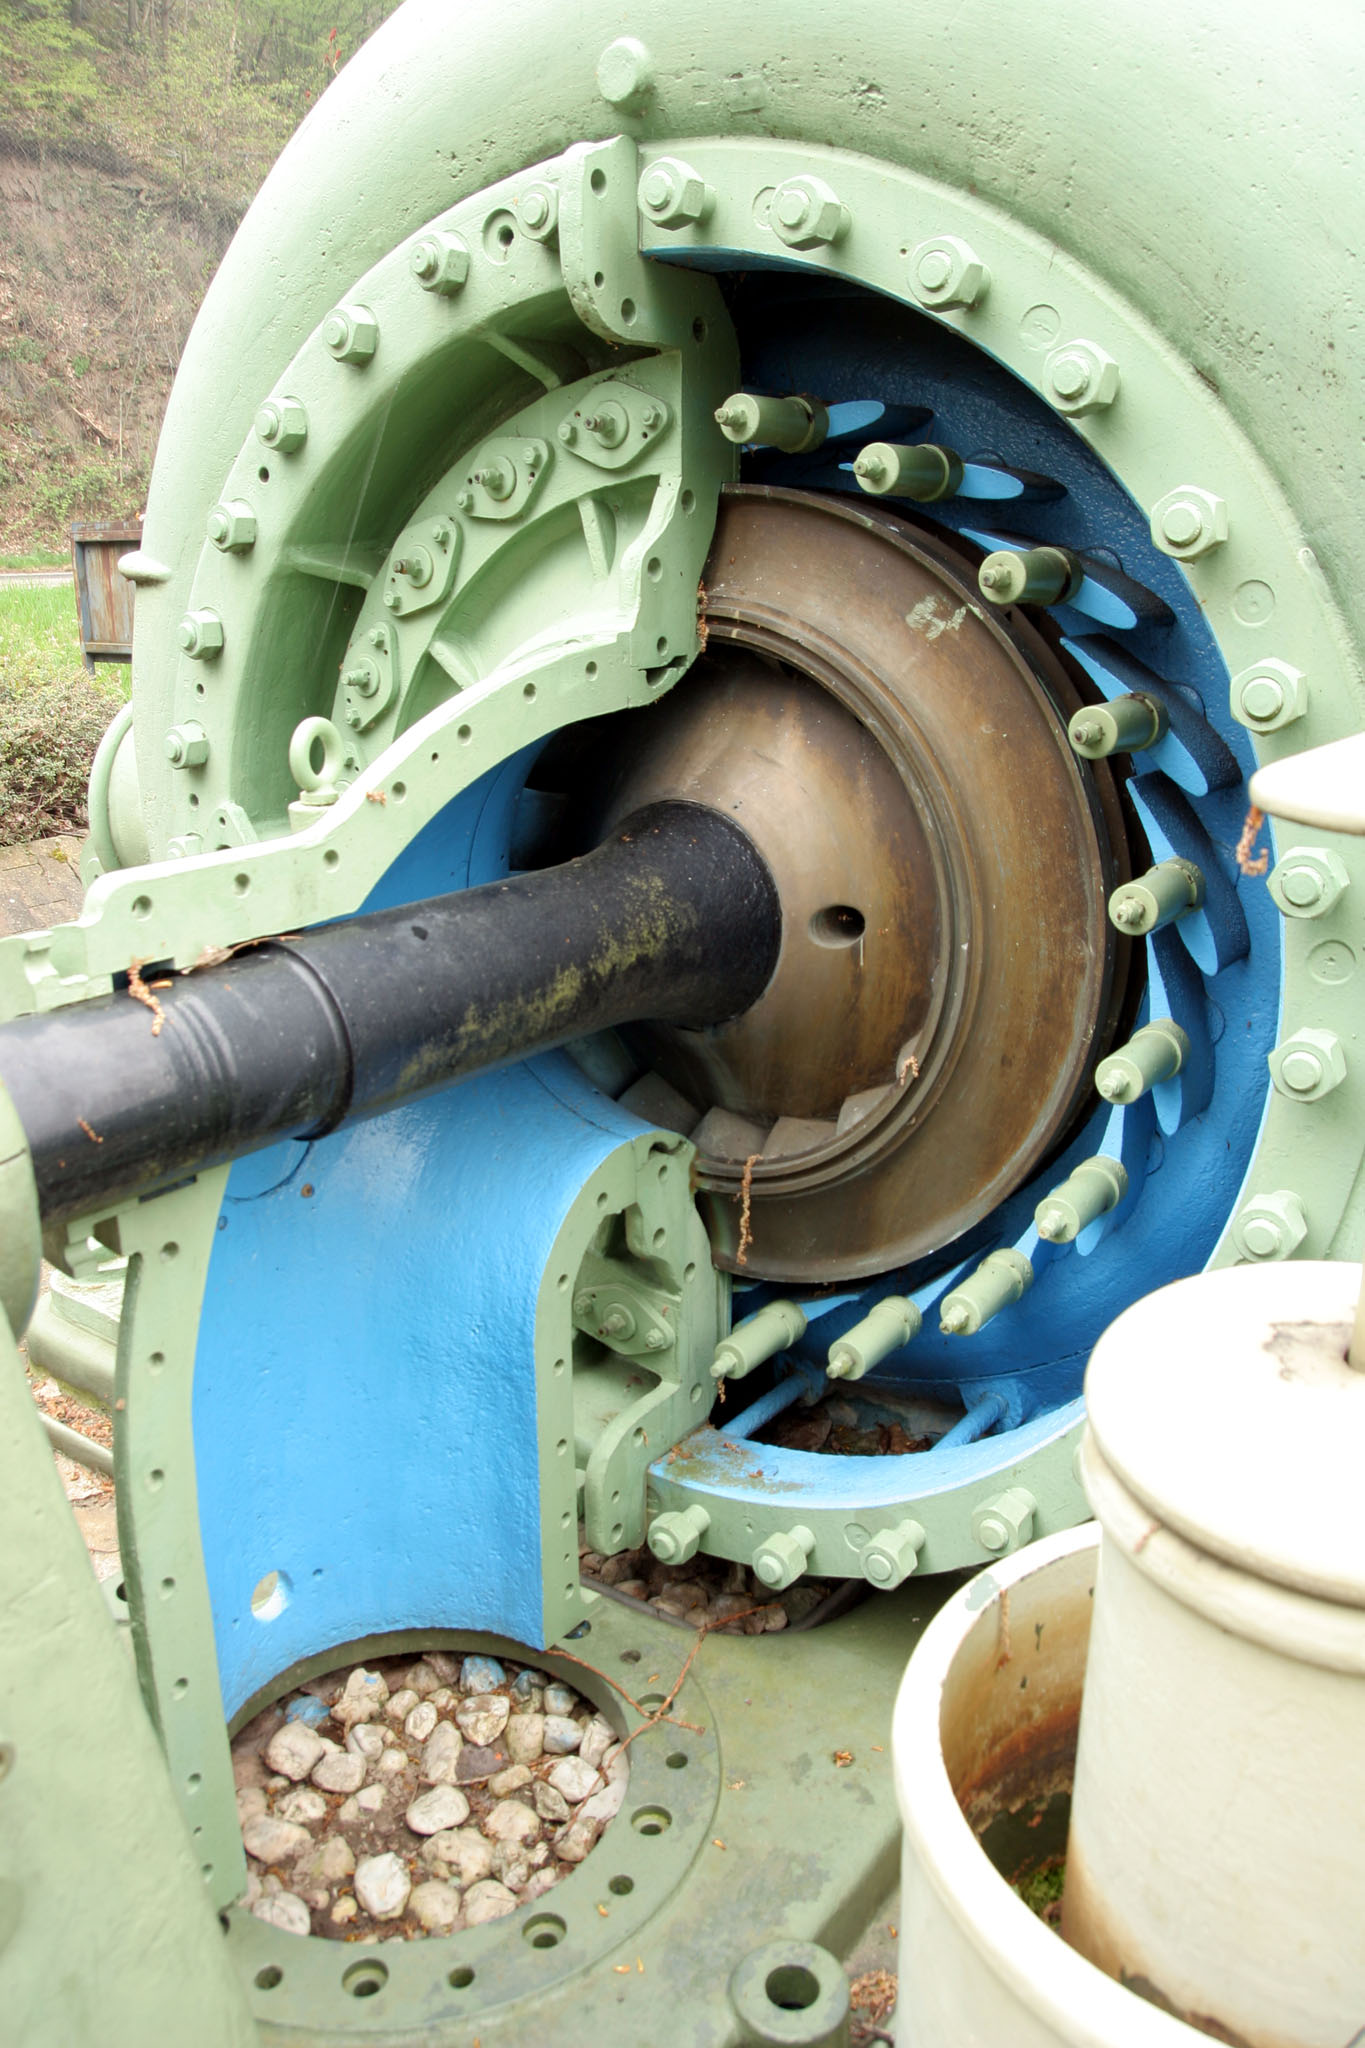
\includegraphics[width = 0.9\textwidth]{report/figures/introduction/francis_turbine.jpg}
                \caption{Cross section of a Francis turbine. The guide vanes are seen in almost closed position. By Armin Kübelbeck.\footnote{Licensed under CC-BY-SA, Wikimedia Commons, \url{https://commons.wikimedia.org/wiki/File:Fankel_Francisturbine_01.jpg}}}
                \label{fig:francis}
            \end{minipage}
            \hfill\vline\hfill
            \begin{minipage}[b]{0.49\linewidth}
                \centering
                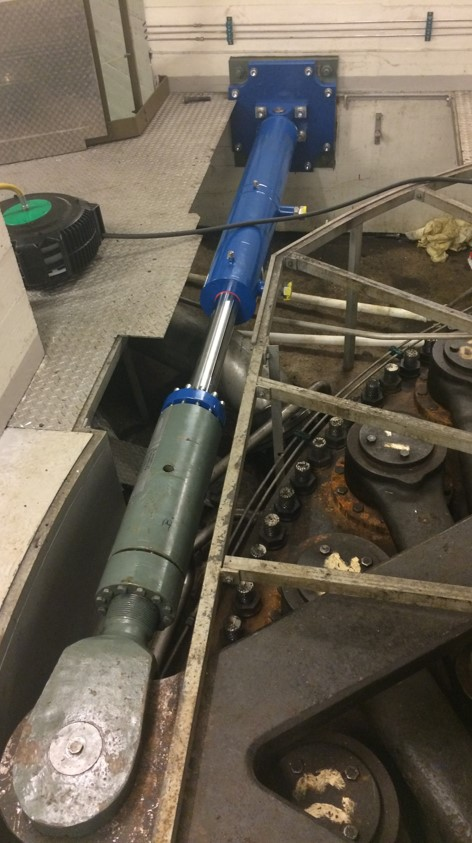
\includegraphics[width = 0.9\textwidth]{report/figures/introduction/servo1(1).jpg}
                \caption{Hydraulic actuator for guide vane control. The actuator is mounted to a ring that controls the guide vane opening. Courtesy of Hymatek Controls}
                \label{fig:guide_vanes}
            \end{minipage}
        \end{figure}
        
    \subsection{Other equipment}
        There are several other large components in a hydro-electrical power plant. Among them are;
        \begin{itemize}
            \item Generators
            \item Transformers
            \item Coolers
            \item Hydraulic systems
        \end{itemize}
    
    \section{Condition monitoring for hydroelectric power plants}\label{sec:cm}
        \cite{Selak2014} presents a complete condition monitoring and fault detection system for hydroelectric power plants, covering everything from data acquisition to fault detection methods. Cost reduction, increase in equipment availability and increased performance are presented as the benefits of introducing condition monitoring. They propose using condition monitoring in addition to preventive maintenance and claim that it is the most comprehensive maintenance scheme available. Data is transferred to a virtual diagnostics center, where an SVM is used to diagnose the data. The proposed condition monitoring system is separated into six steps; data acquisition, data analysis and storage, data transferring, data selection, SVM training and SVM testing. It is proposed to sample data in four different ways to reduce the amount of data stored; periodically at a predefined sampling rate, when signal values exceed a threshold, during transients and sudden events. 
        
        Using SVM for fault diagnostics, data that represents all known failure modes, in addition to normal data is needed. This has restricted the work only to include two variables at a time, as this enables scatterplotting variables against each other for visual confirmation of the normal operation. The training cases separate data into four different datasets; All input data, removing low power operations, removing high water flow operations and removing transients between operation regimes. Experts extracted 44 causalities that can be traced to a pair of process variables. Abnormal data is created as a complement to the normal data, by fitting an oversized boundary to the data from normal operation. As the SVM detector is only trained on two classes, data is only evaluated as normal or abnormal. It is claimed that two-dimensional models are sufficient to catch all known failure modes. The choice of using SVM is supported by \cite{Widodo2007} that presents that SVM has been successfully used in the industry for several different use-cases. 
        
        \cite{Molina2000} introduces two NN approaches to integrate into a decision system for hydroelectric power plant management. An expert system, an NN for acoustic prediction and an NN for predictive maintenance are proposed integrated into one system. It is argued that there are non-linear plant dependencies undetectable for a human expert, that the NN can find. As the expert system tries to mimic the response of a human operator, the system suffers from the same limitations as a human operator. Interpreting an expert system is however much more straightforward than interpreting an NN. Therefore a hybrid system is proposed, benefiting from the best of both worlds. The expert system and the NN for predictive maintenance relay on process data from the plant. The NN for acoustic prediction is fed with data recorded from sensors not used in the two other cases. 106 process variables are available for analysis, all are given as input to the NN, but to mimic the limitations of a human operator, the expert system is only considering 15 variables at a time. The NN for predictive maintenance needs data that represent both normal and abnormal data, for all known failure modes. A particular procedure combining expert knowledge and NNs are used to create data vectors with values for all 106 variables for the given errors created by the expert system. Once the error vectors are created, those are used to train the NN. Classes for the acoustic prediction network were created based on an experts classification of the normal and abnormal regime based on the plants generated power. 
        
        The proposed method was applied and test on a plant in Zamora, Spain. It was found that the combination of the NNs and the expert system outperformed a human operator, but the human operator outperformed the methods individually. The NN for predictive maintenance gave the best individual results. The NN for acoustic predictions suffered from variability in the acoustic signals, but showed that it served as a good addition to the two other methods. 
        
        
    
    
    
    \section{Report outline}
    Chapter \ref{cha:litterature} introduces different anomaly detection techniques, and methods for feature selection and dimensionallity. Chapter \ref{cha:implementation} introduces the software and the libraries used in this thesis. Chapter \ref{cha:data} introduces the dataset and the cases analyzed. Chapter \ref{cha:analysis} walks the reader through the analysis before the discussion and conclusion are found in chapters  \ref{cha:discussion} and \ref{cha:conclusions}.  
% \section{Background and Contributions}\label{sec:contributions}
% Here you describe the main contributions of your project work: What are the new results - the achievements - of your work. 

% It is important that you here also clearly describe which background material you have received. Which information, software, equipment etc. have been made available for you, or form the basis for your work. Which help and support have you received, and from who, during your work. For instance: The Matlab simulator used in Section 2 was provided to me by Ph.D. candidate NN, and I have adapted this to the problem in this thesis by modifying...

% \section{Outline}\label{sec:outline}
% The report is organized as follows. In Chapter~\ref{cha:first} a mathematical model is developed to describe the system... In Chapter

    
    \subsection{Francis turbines}\label{subsec:francis}
        The Francis turbine is a reaction turbine. The water is lead onto the turbine through a set of guide vanes connected to the spiral casing, and lead out from the center of the turbine. The guide vanes control the amount of water lead to the turbine, and hence the amount of produced energy. A cross-section of a Francis turbine is seen in Figure \ref{fig:francis}. All guide vanes have the same opening and are controlled through a ring mounted on the top of the turbine. Figure \ref{fig:guide_vanes} shows a hydraulic actuator used to control the ring that operates the guide vanes. As for the Pelton turbine, the hydraulics is again controlled by the plant's control system. \cite{Aasnes2017} tries to classify the condition of the guide vanes in a Francis turbine using different machine learning methods such as support vector machines (SVM), neural networks (NN) and regression.   
        
        \begin{figure}
            \begin{minipage}[b]{0.49\linewidth}
                \centering
                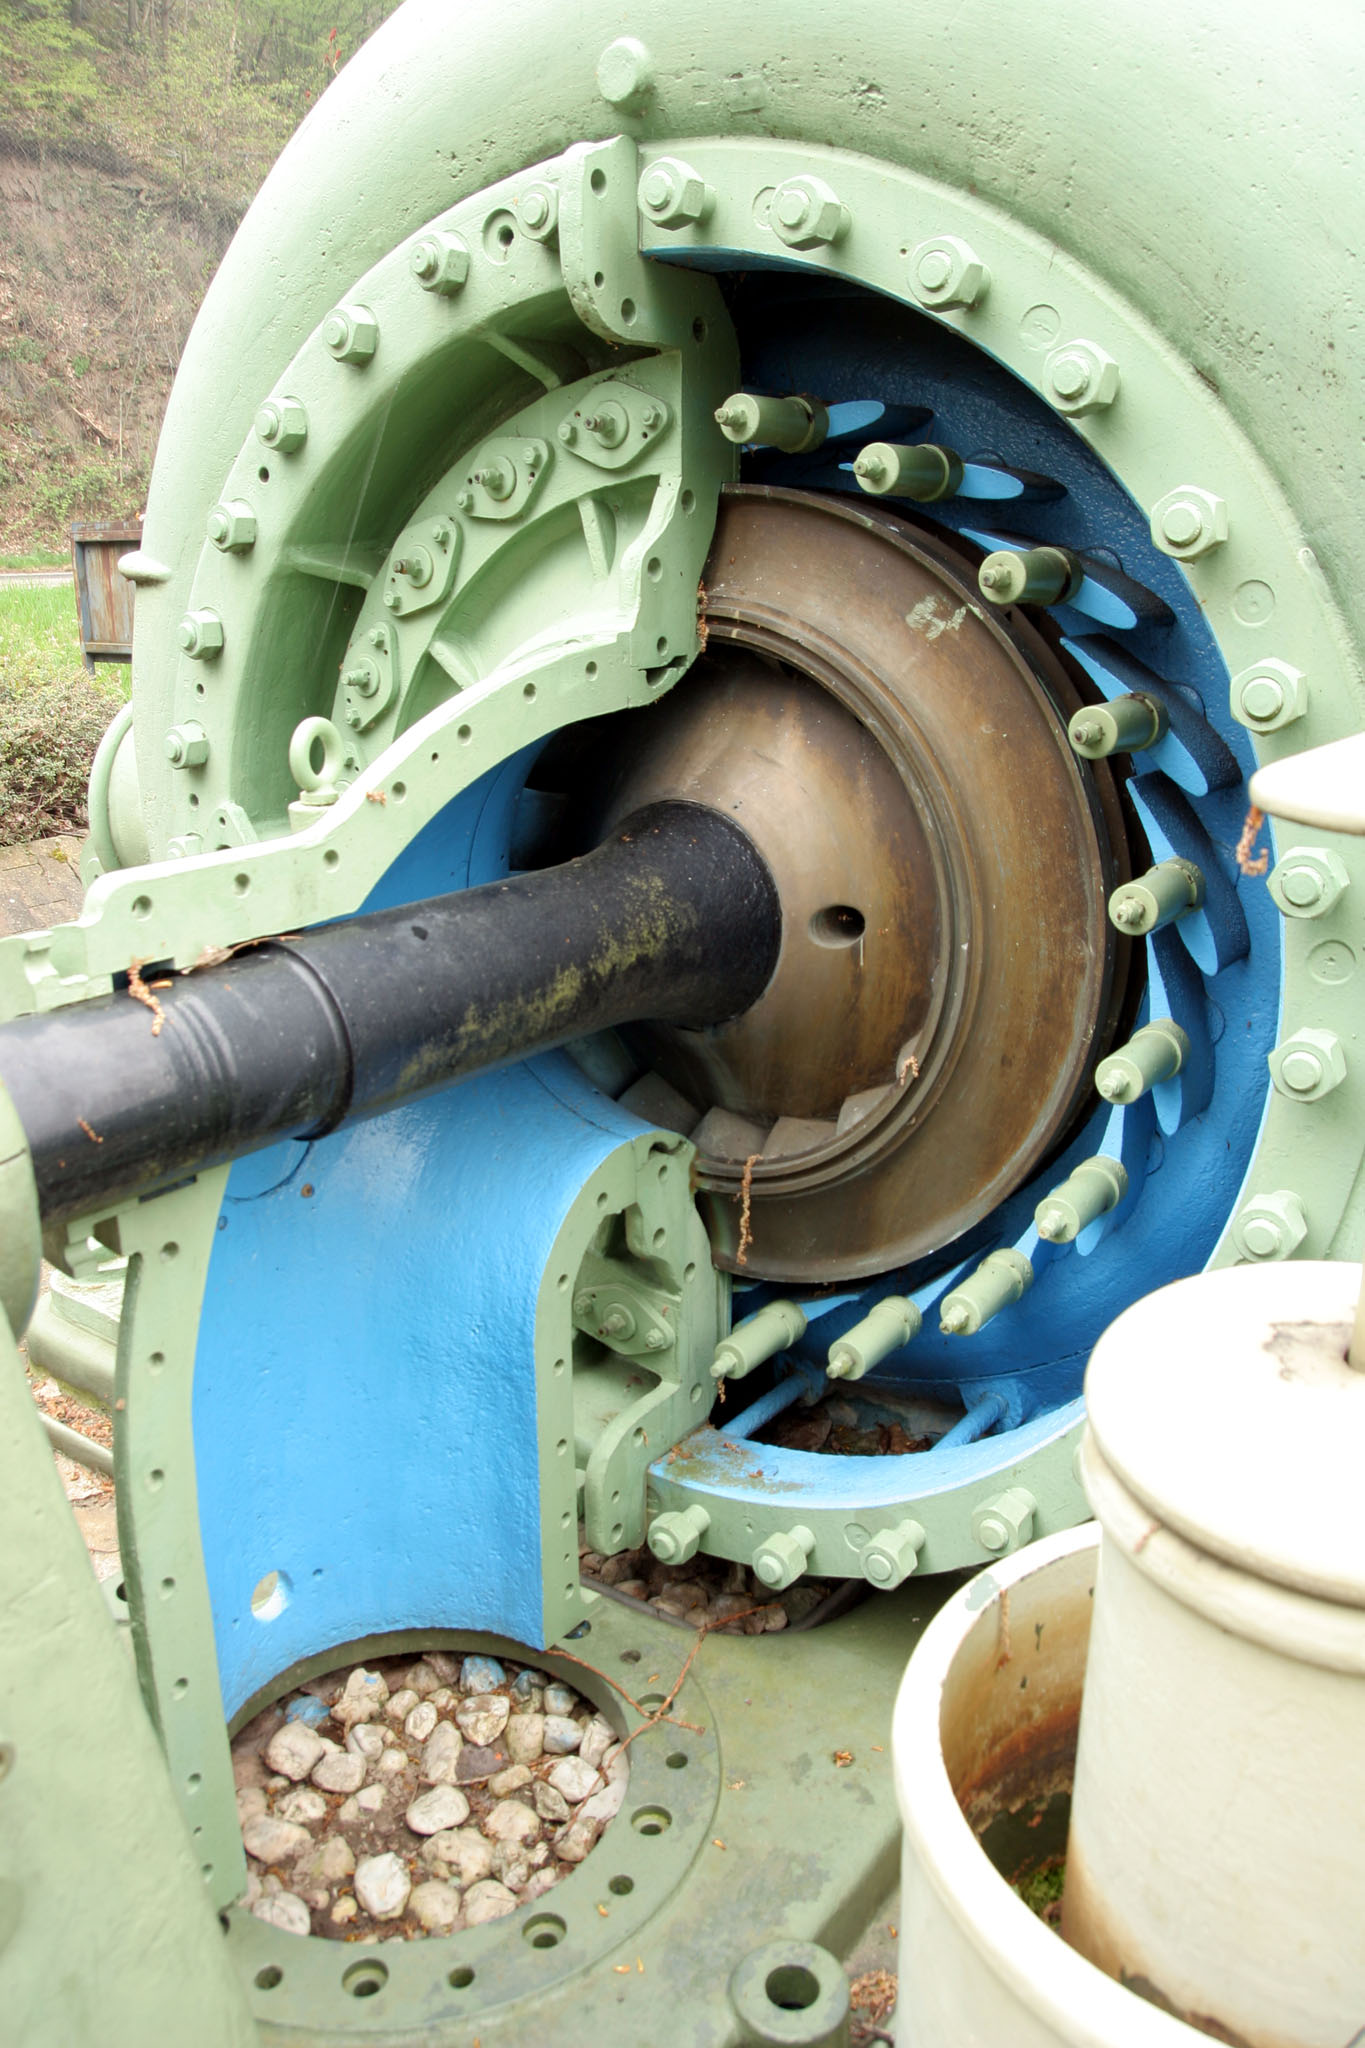
\includegraphics[width = 0.9\textwidth]{report/figures/introduction/francis_turbine.jpg}
                \caption{Cross section of a Francis turbine. The guide vanes are seen in almost closed position. By Armin Kübelbeck.\footnote{Licensed under CC-BY-SA, Wikimedia Commons, \url{https://commons.wikimedia.org/wiki/File:Fankel_Francisturbine_01.jpg}}}
                \label{fig:francis}
            \end{minipage}
            \hfill\vline\hfill
            \begin{minipage}[b]{0.49\linewidth}
                \centering
                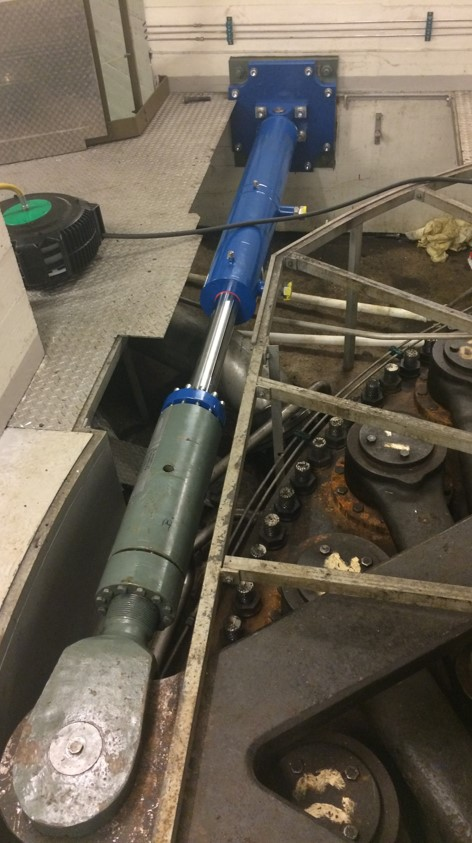
\includegraphics[width = 0.9\textwidth]{report/figures/introduction/servo1(1).jpg}
                \caption{Hydraulic actuator for guide vane control. The actuator is mounted to a ring that controls the guide vane opening. Courtesy of Hymatek Controls}
                \label{fig:guide_vanes}
            \end{minipage}
        \end{figure}
        
    \subsection{Other equipment}
        There are several other large components in a hydro-electrical power plant. Among them are;
        \begin{itemize}
            \item Generators
            \item Transformers
            \item Coolers
            \item Hydraulic systems
        \end{itemize}
    
    \section{Condition monitoring for hydroelectric power plants}\label{sec:cm}
        \cite{Selak2014} presents a complete condition monitoring and fault detection system for hydroelectric power plants, covering everything from data acquisition to fault detection methods. Cost reduction, increase in equipment availability and increased performance are presented as the benefits of introducing condition monitoring. They propose using condition monitoring in addition to preventive maintenance and claim that it is the most comprehensive maintenance scheme available. Data is transferred to a virtual diagnostics center, where a SVM is used to diagnose the data. The proposed condition monitoring system is separated into six steps; data acquisition, data analysis and storage, data transferring, data selection, SVM training and SVM testing. It is proposed to sample data in four different ways to reduce the amount of data stored; periodically at a predefined sampling rate, when signal values exceed a threshold, during transients and during sudden events. 
        
        Using SVM for fault diagnostics, data that represents all known failure modes, in addition to normal data is needed. This has restricted the work to only include two variables at a time, as this enables scatterplotting variables against each other for visual confirmation of the normal operation. The training cases separate data into four different datasets; All input data, removing low power operations, removing high water flow operations and removing transients between operation regimes. Experts extracted 44 causalities that can be traced to a pair of process variables. Abnormal data is created as a complement to the normal data, by fitting an oversized boundary to the data from normal operation. As the SVM detector is only trained on two classes, data is only evaluated as normal or abnormal. It is claimed that two-dimensional models are sufficient to catch all known failure modes. The choice of using SVM is supported by \cite{Widodo2007} that presents that SVM has been successfully used in the industry for several different use-cases. 
        
        \cite{Molina2000} introduces two NN approaches to integrate into a decision system for hydroelectric power plant management. An expert system, a NN for acoustic prediction and a NN for predictive maintenance are proposed integrated into one system. It is argued that there are non-linear plant dependencies undetectable for a human expert, that the NN can find. As the expert system tries to mimic the response of a human operator the system suffers from the same limitations as a human operator. Interpreting an expert system is however much easier than interpreting a NN, therefore a hybrid system is proposed, benefiting from the best of both worlds. The expert system and the NN for predictive maintenance relay on process data from the plant. The NN for acoustic prediction is fed with data recorded from sensors not used in the two other cases. 106 process variables are available for analysis, all are given as input to the NN, but to mimic the limitations of a human operator, the expert system is only considering 15 variables at a time. The NN for predictive maintenance needs data that represent both normal and abnormal data, for all known failure modes. A special procedure combining expert knowledge and NNs are used to create data vectors with values for all 106 variables for the given errors created by the expert system. Once the error vectors are created, those are used to train the NN. Classes for the acoustic prediction network were created based on an experts classification of the normal and abnormal regime based on the plants generated power. 
        
        The proposed method was applied and test on a plant in Zamora, Spain. It was found that the combination of the NNs and the expert system outperformed a human operator, but the human operator outperformed the methods individually. The NN for predictive maintenance gave the best individual results. The NN for acoustic predictions suffered from variability in the acoustic signals, but showed that it served as a good addition to the two other methods. 
        
        
    
    
    
    \section{Report outline}
    Chapter \ref{cha:litterature} introduces different anomaly detection techniques, and methods for feature selection and dimensionallity. Chapter \ref{cha:implementation} introduces the software and the libraries used in this thesis. Chapter \ref{cha:data} introduces the dataset and the cases analyzed. Chapter \ref{cha:analysis} walks the reader through the analysis before the discussion and conclusion are found in chapters  \ref{cha:discussion} and \ref{cha:conclusions}.  
% \section{Background and Contributions}\label{sec:contributions}
% Here you describe the main contributions of your project work: What are the new results - the achievements - of your work. 

% It is important that you here also clearly describe which background material you have received. Which information, software, equipment etc. have been made available for you, or form the basis for your work. Which help and support have you received, and from who, during your work. For instance: The Matlab simulator used in Section 2 was provided to me by Ph.D. candidate NN, and I have adapted this to the problem in this thesis by modifying...

% \section{Outline}\label{sec:outline}
% The report is organized as follows. In Chapter~\ref{cha:first} a mathematical model is developed to describe the system... In Chapter

\chapter{Theory}\label{cha:litterature}

This chapter introduces three anomaly detection techniques that can be used for condition monitoring, and methods for feature extraction and dimensionality reduction to be used in addition to the anomaly detection techniques. 


\section{Anomaly detection}\label{sec:novelty_detection}
    \cite{Pimentel2014} defines anomaly detection as the task of classifying test data that in some way differs from data used for training, hence this is one obvious approach to condition monitoring. This is like a one-sided test or one class classification. This means that one is not training on data that represents fault, only on data sampled from normal operation. As a model describing the normal operation of the system is learned, it is essential that one has samples of normal system behavior for all the possible states of operation. Anomaly detection avoids the issue with finding data that represents all possible failure modes. Such techniques are very valuable for industrial applications, where the need for failure detection is great, but identifying all possible failure modes and collecting data to represent them can be difficult and very costly. It is much easier to get measurements from a machine during normal operation, than during failure, and it is in many cases close to impossible to obtain as many samples of negative or faulty behavior as of normal behavior. \cite{Tarassenko2009} claims that modern high-integrity systems are so complex that they introduce many possible failure modes that are not very well captured by the instrumentation available. This can be verified by visiting a hydroelectric power plant. There is much instrumentation, and many alarms for different components, but all of these are linked to well-known failure modes. Anomaly detection introduces the possibility to detect unknown abnormalities. It is, however, important to notice that anomaly detection methods are prone to suffer from a higher rate of false positives than when abnormal data is available for training \cite{Latecki}. The performance of the anomaly detection is dependent on the choice of parameters, and it is essential to keep in mind whether it is false negatives or false positives that are of the highest concern 
    
    Since anomaly detection techniques are based on "normal" system behavior, they should, in theory, be able to detect any failure mode that can occur, if provided with the correct process information. Adding process signals that are not known to be connected to any of the known failure modes can be beneficial for such methods. This also makes sense when one does not know what to look for. One wants all possible information available. This leads to a significant remark, only getting a notification that an anomaly is observed, does not provide very much information. For these techniques to have any real value, one needs to be able to trace which component the anomaly comes from, and the magnitude of the anomaly. Once the anomaly detection techniques are trained, new data are given a novelty score based on how well they compare to the normal description of the system. This score can then be compared to a threshold, and the data will be marked as normal or abnormal. Using anomaly detection techniques avoids having to create data that represent the failure modes as seen in \ref{sec:cm}. This means that the methods are more straightforward to generalize and adapt to new uses. 

    Many of the techniques in the following sections are based on the suggestions from \cite{Pimentel2014} which provides an extensive review of novelty detection. 

\section{Reducing the input space}\label{sec:reduce_features}
    As the size of the input grows, the complexity and runtime of the techniques grow with it. It can become necessary to reduce the input space of the anomaly detection techniques to ensure reasonable run time. Interpreting and visualizing data of high dimensions is difficult. The feature size also introduces issues regarding memory and algorithm runtime, \cite{Guyon2003} and \cite{Dy2004}. Reducing the complexity of the problem is heavily correlated with reducing the number of features. Feature selection techniques can also reveal unknown plant dynamics which can help to understand why some components fail.
    
    "The problem is that not all features are important. Some of the features may be redundant, some may be irrelevant, and some can even misguide clustering results" from \cite{Dy2004} sums up one of the issues with datasets with many features. A concrete example of this is shown in Figure \ref{fig:feature_selection}, her one can clearly see that $X_2$ does not provide any information on how the data points are clustered. Including this feature in a learning algorithm does not provide any information about the two classes found in the dataset, hence in the best case, the performance will be the same as if only $X_1$ was used. This is supported by \cite{Liu2010} that states that some features can be removed without lowering the performance of a learning algorithm.
    
    \begin{figure}
        \centering
        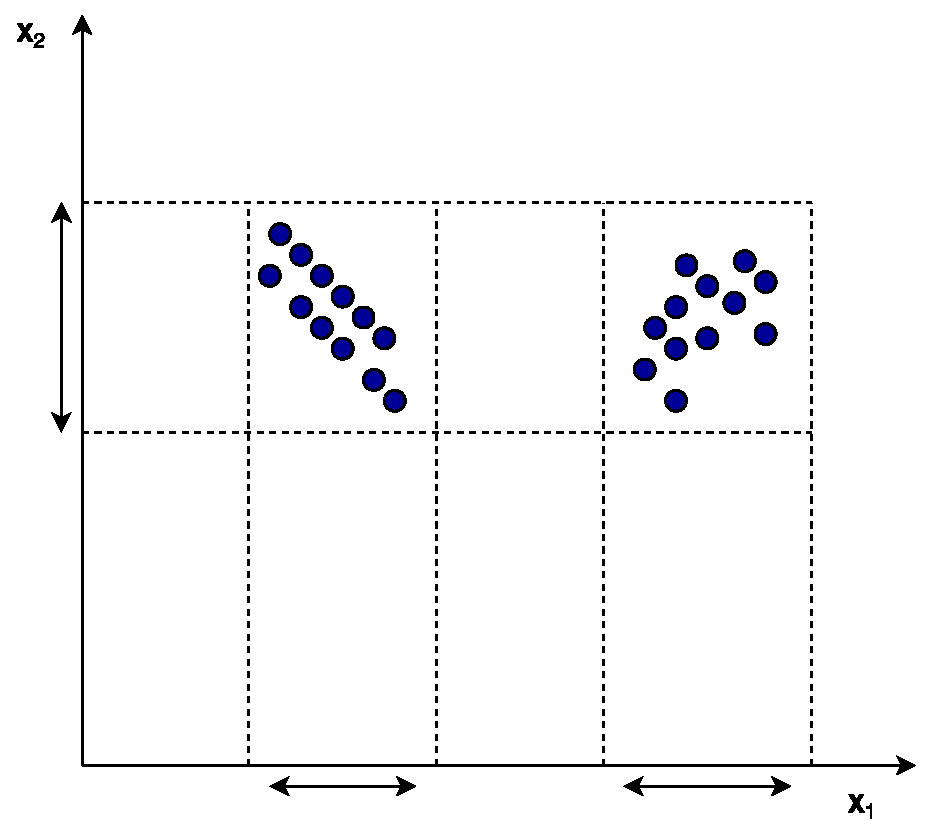
\includegraphics[width=0.5\textwidth]{report/figures/techniques/feature_selection.pdf}
        \caption{Example of a dataset with two features, one relevant and one irrelevant feature}
        \label{fig:feature_selection}
    \end{figure}
    
    There are two main techniques for reducing the input space, feature selection and dimensionality reduction. The former, try to remove the least informative and the redundant features from the feature set. The latter creates new features either as linear or non-linear combinations of the original feature set, hence one can remove the dimensions with little variance. Feature selection is again separated into a supervised and non-supervised selection. In the supervised case, one has a set of features and a target variable, hence one want to keep the features that are related to the target variable. For unsupervised feature selection, there is no target variable to help remove uninformative or redundant features, and other factors must be used for selection.
    
    
    \subsection{Filter, wrapper and embedded methods}\label{subsec:filter_wrapper_embedded}
        The different classes or types of methods for feature reduction are split into three groups, filter, wrapper and embedded methods. This section will give a short introduction to each of them.
        According to \cite{Liu2010} filter methods are methods that perform feature selection separate from the learning algorithm, and hence can be used no matter which learning algorithm is applied later. The wrapper methods, however, need a predetermined learning algorithm. The features are then selected based upon the performance of the chosen algorithm.  Finally, the embedded methods incorporate the selection of features in the training of the learning algorithms model. \cite{Liu2010} also states that since the filter methods are independent of the learning algorithm they are not biased with regard to the algorithm, this means that filter methods are to prefer when the learning algorithms are not known beforehand. 
\section{Supervised feature selection}\label{sec:sup_feat_select}
    Supervised feature selection can be used when one has a target to track. This means that one needs to identify a process signal or a function of a process signal of interest which one want to trace in the other process variables. An example is anomaly detection for a bearing. By using process variables from the bearing such as vibration and temperature, one can find other process variables that are in some way related to the targets. This section introduces two supervised feature selection methods. 
    % As seen in chapter \ref{cha:data} the control problems with the needles can be observed in the difference or the RMSE between the pairwise controlled needles. Using the RMSE between the needles as a target variable enables the use of supervised feature selection algorithms. 
    
    
    \subsection{K-best using correlation and  mutual information}\label{subsec:K-best_feat_select}
    
        Mutual information (MI), \cite{Kraskov2004} and \cite{Peng2005} explains how dependent or inversely how independent two variables are. It gives an understanding of how much knowing something about one variable reduces the uncertainty about the other. If two variables are completely independent, their corresponding MI. 
        
        The MI is defined as
        \begin{align}\label{eq:tech_MI}
                MI(X,Y) = \int \int p(x,y) \log \frac{p(x,y)}{p_x(x)p_y(y)},
        \end{align}
        where $x$ and $y$ are the two variables to compare, and $p_x(x)$ and $p_y(y)$ are their corresponding probability density functions. One benefit from MI is that does not only find linear correlation between two variables. In other words, it finds dependencies between variables not necessarily shown in correlation, meaning that this serves as complementary technique to using co-variance or correlation for feature selection, \cite{Li}. The K features with highest MI will be chosen. 
        
        
        The K-best features can also be selected using the above-mentioned correlation. The correlation between a feature and the target variable is found as  
        \begin{align}
            corr(X,Y) = \frac{cov(X,Y}{\sigma_x\sigma_y} = \frac{E[(X-\mu_x)(Y-\mu_y)]}{\sigma_x\sigma_y}.
        \end{align}
        Here the K features with highest correlation with the target variable will be chosen. 
        
\section{Unsupervised feature selection}\label{sec:unsup_feat_reduc}
    Unsupervised feature selection is harder than supervised feature selection. The lack of a target variable removes the ability to interpret which variable dynamics that are important easily. Still, the need to reduce the feature set is prominent. \cite{Dy2004} describes the problem as follows, "The goal of feature selection for unsupervised learning is to find the smallest feature subset that best uncovers “interesting natural” groupings (clusters) from data according to the chosen criterion." The chosen criterion defines what is thought to be interesting natural groupings. There is no golden rule for defining this criterion, and a subset that is good for one purpose might not be relevant for others. Two possible methods for unsupervised feature selection follows.
    
    
    \subsection{K-best using variance threshold}\label{subsec:var_thres}
        Variance threshold removes merely the features with the lowest variance. According to \cite{He2005} it is one of the most straightforward evaluation methods for unsupervised selection. One of the drawbacks of using variance to select features is that there might be many features with large variances that is non-informative with what one is looking for. The algorithm is very simple, and it returns the k features that have the highest variance. 
        
    
    \subsection{Laplacian score}\label{subsec:lapl_score}
        Laplacian score for feature selection was proposed as an alternative to unsupervised feature selection by \cite{He2005}. The method builds upon the assumption that features belonging to the same class or grouping can be found close together. The features are evaluated based on how well locality is preserved, which is found by the Laplacian score. The Laplacian score is calculated for each feature. A short introduction to the method is described below. More details is found in \cite{He2005}. 
        
        Laplacian score is based on Laplacian Eigenmaps, which is an algorithm for dimensionality reduction. The algorithm creates a nearest neighbors graph with a node for each sample of each feature. Hence the dimension becomes $m$ times the number of features. Two nodes share an edge if they are among the k-nearest neighbors to each other, meaning that k is one of the tunable parameters for this algorithm. Each edge is then given a weight based on the Gaussian radial basis function;
        
        \begin{align}\label{eq:tech_LS}
            W_{i,j} = e^-{\frac{||{\bm{X_i}-\bm{X_j}}^2||}{t}},
        \end{align}
        
where t is another tunable parameter. Then a graph Laplacian is computed which then again is used to calculate a Laplacian score. As mentioned the algorithm has two tunable parameters. The main reason for choosing Laplacian score as one of the unsupervised feature selection methods is that it can compare and rate features against each other. This introduces a new dimension compared to the more naive variance threshold algorithm that only looks at one feature at a time. 
    

\section{Dimensionality reduction}\label{sec:dim_red}
    One of the issues with feature reduction is that the features that are removed may hold information that could help the learning algorithm. In dimensional reduction, the feature set is used to create new features which means that a new reduced feature space of dimension n can hold the same amount of information as the original feature space of size m, $m>n$.

    \subsection{Principal component analysis}\label{subsec:PCA}
        Principal component analysis (PCA) is a popular technique used for dimensional reduction. PCA is an orthogonal transformation that takes a set of possibly correlated variables, and transforms them into a set of noncorrelated components, effectively reducing the dimensions of the data. These new dimensions are known as principal components. There are several different algorithms that can be used to calculate the principal components, one of them is singular value decomposition or SVD. SVD decomposed the data into eigenvalues and eigenvectors. The larger an eigenvalue is, the better its corresponding eigenvector capture the variance of the data. All eigenvectors are orthogonal, this means that each vector introduces an entirely new dimension. In a high dimensional dataset with many features, there will most likely be features that are fairly similar. Figure \ref{fig:tech:PCA} shows intuitively how the PCA algorithm works. Data samples from a dataset with three features are shown in the plot. As the principal components in red and green shows, most of the variance in the samples can be represented using only one dimension. Adding the second dimension, only small residuals might be left. This illustrates how the PCA algorithm operates. 
        
        \begin{figure}
            \centering
            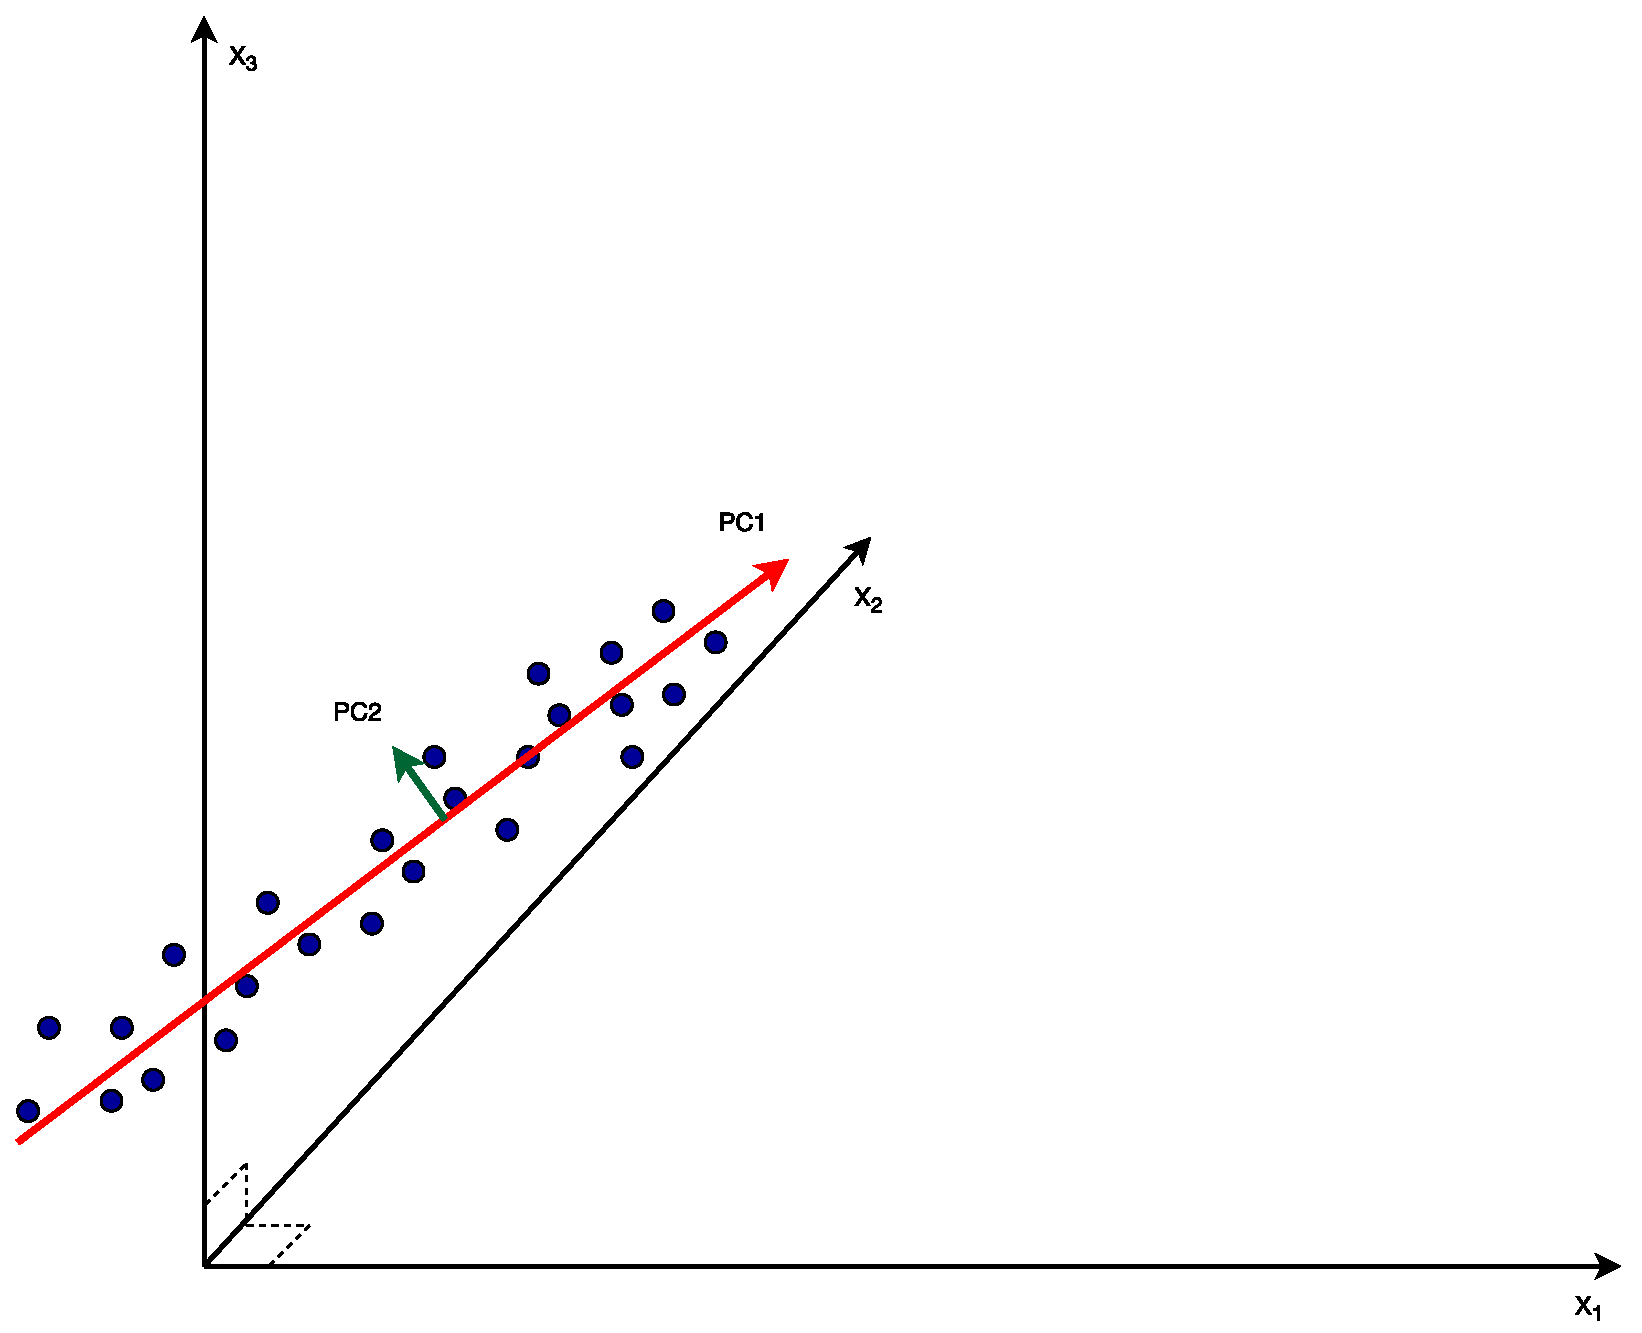
\includegraphics[width=\textwidth]{report/figures/techniques/PCA.pdf}
            \caption{Illustration of principal component analysis. The two principal components are seen in red and green. Using only PC1 most of the variance in the data is still kept.}
            \label{fig:tech:PCA}
        \end{figure}
        
        

    
    \subsection{Kernel principal component analysis}\label{subsec:kernelPCA}
        Kernel PCA builds upon the PCA algorithm explained above, but it introduces a new trick. Where PCA is only able to create new features from linear combinations of the original feature set, kernel PCA uses the kernel trick to enable non-linear combinations as well. Take a two-dimensional dataset containing samples from two different classes.  These classes are only linearly separable if the classes can be separated by a line. If one class surrounds the other class, there is no way to linearly separate the two classes in two dimensions. However, by extending the sample space into three dimensions, it might now be possible to separate the two classes with a hyperplane. Hence making a non-linear separation of the two classes possible, by still using linear methods. If the datasets are large, transforming all samples into a higher dimension can become computationally heavy. The kernel trick solves this problem without having to transform the samples. The kernel PCA extends the original PCA to a higher dimension using the kernel trick, enabling the extraction of nonlinear components.  
    
        By mapping the original data nonlinearly into a new feature space $F$ $\phi(\bm{x_1})$, and by performing PCA in this new feature space, one can get nonlinear principal components.


\section{Anomaly detection techniques}
    In this section, three different techniques for anomaly detection is presented. SVM is a classifying algorithm that automatically classifies data as either normal or an anomaly. \cite{Selak2014} uses SVM for condition monitoring. One Class Support Vector Machine (OCSVM) is presented as it only needs normal training data, removing the need for artificially creating data for known failure modes. Kernel density estimation (KDE) is a method for estimating the probability density function or pdf of a set of variables. New data can then be evaluated on how well it fits the learned pdf. Long short term memory recurrent neural network is neural network designed for learning time series data. 

    \subsection{One class support vector machine}\label{subsec:OCSVM}
    
            The following section is a based on \cite{Aasnes2017} and \cite{Hastie}. 
            
            SVMs can be used for data belonging to one or more classes. The SVM algorithm defines a hyperplane that best separates two different classes. Hence data is labeled normal or abnormal based on which side of the hyperplane it lays. In anomaly detection only normal data is available. Hence one has no negative data to help to fit the hyperplane. SVM is capable of separating data both linearly and non-linearly. A kernel function, or a similarity function, describes how similar two feature vectors are by taking the inner product of the two samples in a higher dimensional space. The kernel function does this without having to transform the data into this dimension explicitly. Two commonly used kernels are the Gaussian kernel
            \begin{align}
                K_g(\bm x^{1},\bm x^{2}) = e^{\frac{\norm{\bm x^{1}-\bm x^{2}}^2}{2\sigma^2}}, 
                \label{svm:gauss}
            \end{align}
            and the polynomial kernel
            \begin{align}
                K_p(\bm x^{1},\bm x^{2}) = (\bm x^{1T}\bm x^{2} + \alpha)^\beta.
                \label{svm:poly}
            \end{align}
           These are just two of many examples. The Gaussian or RBF kernell is a good first choice if you know that you have a nonlinear boundary, but don't know exactly what shape the boundary will take.
    
            \begin{align}
                f(\bm x) = \beta_0 + \bm \beta^T\bm x = 0,
                \label{svm:hyper}
            \end{align}
            defines a hyperplane. For any two feature vectors $\bm x^{[1]},\bm x^{[2]}$ that lie in or on the hyperplane where $\bm \hat x = \bm x^{[1]} - \bm x^{[2]}$, gives  $\bm \beta^T \bm \hat x = 0 $ and hence, $\bm \beta$ is a scalar multiplication of the normal vector to the hyperplane. Where
            \begin{align}
                \bm \beta^* = \frac{\bm \beta}{\norm{\bm \beta}}
                \label{svm:norm}
            \end{align}
            is the normal vector. Inserting any feature point $\bm x_0$ that lies on or in the hyperplane defined by Equation \ref{svm:hyper}, yields $\bm \beta^T\bm x_0 = -\bm \beta_0$. By using $\bm x_0$ as any feature vector from origo to the hyperplane and the normal vector $\bm \beta^*$, the distance for any given feature vector $\bm x$ to the hyperplane is given by
            \begin{align}
                \bm \beta^{*T}(\bm x - \bm x_0) = & \frac{\bm \beta^T}{\norm{\bm \beta}} (\bm x - \bm x_0) \nonumber \\
                % = & \frac{1}{\norm{\bm \beta}}(\bm \beta^T\bm x- \bm \beta^T\bm x_0) \nonumber \\
                % = & \frac{1}{\norm{\bm \beta}}(\bm \beta^T\bm x + \bm \beta_0) \nonumber \\
                = & \frac{1}{\norm{f'(\bm x)}}f(\bm x).
                \label{svm:dist}
            \end{align}
            
            A decision rule 
            \begin{align}
                y^i(\bm x^{iT} \bm \beta + \beta_0) \geq 0 
                \label{svm:decision}
            \end{align}
            can then be created using the hyperplane. Since there are two classes they are defined as $y_0 = 1$ and $y_1 = -1$. The decision rule tells which class a feature vector belongs to. Note that points belonging to the negative class should yield negative distance to the hyperplane, and hence the decision rule ensures that all points are classified correctly.
            
            Now that an expression for the distance from a hyperplane to any given feature vector in the feature space is defined, one can look at how to find the optimal hyperplane to separate the two classes. The margin or the width between the two closest point from both classes can be defined as $M = \frac{2}{\norm{\bm \beta}}$, and hence maximizing the distance can be formulated as minimizing
            \begin{align}
                J(\bm \beta) = & \frac{1}{2}\norm{\bm \beta}^2 \nonumber \\
                 s.t \quad y^i(\bm \beta^T\bm x^i + \beta_0) \geq & 1 \quad \forall \enspace i.
                \label{svm:cost}
            \end{align}
            The constraint here ensures that every point is classified correctly. Having to classify all samples correctly can lead to a very complex boundary or hyperplane, in addition there is always a risk that data is labeled incorrectly. Therefore slack variables are added to enable some wrong classifications as seen in the updated minimization problem
            \begin{align}
                J(\bm \beta) = & \frac{1}{2}\norm{\bm \beta}^2  + C \sum_{i=1}^N \xi_i \nonumber \\
                 s.t \quad \xi_i \geq 0, y^i(\bm \beta^T\bm x^i + \beta_0) \geq & 1 - \xi_i \quad \forall \enspace i.
                \label{svm:cost}
            \end{align}
            % The solutution to the original SVM algorithm is found by a Lagrangian optimization problem which maximize distance between two classes as, 
            %  \begin{align}
            %     L = \sum_{i=1}^n  \alpha_i - \frac{1}{2} \sum_{i=1}^n \sum_{j=1}^n \alpha_i \alpha_j y^i y^j \bm x^{i}^T \bm x^j,
            %     \label{svm:dual}
            % \end{align}
            % or by 
            % \begin{align}
            %     L = \sum_{i=1}^n  \alpha_i - \frac{1}{2} \sum_{i=1}^n \sum_{j=1}^n \alpha_i \alpha_j y^i y^j K(\bm x^{i}, \bm x^j)
            % \end{align}
            % if the kernel trick is used. Here $\alpha$ are the parameters that defines the separating hyperplane, and it is constrained by having to correctly classify data to its original class. Both are a convex optimization problem which has the nice attribute of having a global maxima. This means that you will always find the best solution for the given parameters.
            
            In the case of OCSVM, \cite{Scholkopf2001}, there is only one class available, so the problem is formulated slightly different,
            \begin{align}
                \min \quad J(\bm \beta) = & \frac{1}{2}\norm{\bm \beta}^2  + \frac{1}{\nu N}\sum_{i=1}^N \xi_i - \rho \nonumber \\
                s.t \quad (\beta \cdot \phi(x_i) \geq & \rho - \xi_i \quad \forall \enspace i \nonumber \\
                \xi_i \geq & 0 \quad \forall \enspace i.
                \label{svm:cost_oc}
            \end{align}
            The main difference is the parameter $\nu$ wich serves as a upper fractional bound for accepted number of outliers, and as a lower bound for the fraction of support vectors used by the algorithm. $\rho$ is simply an offset. OCSVM is typically trained on normal data, fitting the decision boundary close to the normal data pattern. Anomalies that deviate from the normal data will then be found on the other side of the separating hyperplane, and classified as an anomaly.    
            % If your classes are not linearly separable in the feature space, maximization of Equation \ref{svm:dual} has no global solution. However as can be seen in Equation \ref{svm:dual} one want to minimize $\bm x_i^T  \bm x_j$. This term can then be replaced by one of the kernel functions defined above, which now enables separation in a higher dimensional space.
            
            % The final thing to remark is that not all datasets are entirely separable, to deal with this a slack variable is introduced into the optimization to allow miss-classification of some of the feature vectors. 
        
    
        % One issue with one class SVM combined with non labeled data is that hyperparameterization becomes hard. There is no out of the box scoring function that tells how well the classifier is performing. As long as one is working in two or three dimensions, it is possible to plot the decision boundary, and select parameterization based on visual observations. In higher dimensions, this becomes a problem. Therefore a new method is proposed used to reduce the number of hyperparameterizations to consider. A score is given to each of the parameterizations from
        
        % \begin{align}
        %     score = \abs\sigma + \mu + 100\frac{outliers}{inliers},
        % \end{align}
        % where the lower the score, the better the performance. $\sigma$ here represents the standard deviation of the distances from the decision boundary, $\mu$ is the unsigned distance to the decision boundary. These values were picked because the training data is said to be normal operation, and should not contain any outliers. However, this leads to the risk of a too general boundary where the classifier is no longer able to predict outliers. This means that the closer the boundary is to the samples in the training data, the higher the score. The final fraction of outliers and inliers is added to make sure that most of the data is classified as inliers. If not on runs the risk of fitting a very complex boundary which yields good distance measures for all samples, this will, however, lead to a large fraction of outliers which is not the case for the normal training data. 
        
        
    
    \subsection{Kernel density estimation}\label{subsec:kde}
        KDE, \cite{Latecki}, creates an estimate of the probability density function or pdf of the data. The data is then evaluated by how likely it is to belong to the estimated density function. This is a non-parametric technique meaning that the data is not assumed to take the shape of a given distribution. The probability density function is estimated using a set of kernels that are distributed across the data. The probability density is then estimated at each kernel location based on data that lie within a local neighborhood of the kernel. The density found at a point x within its neighboring n points is given by, 
        \begin{align}
            \hat{f}(x) = \frac{1}{n} \sum_{i=1}^n K_h(x-x_i)  = \frac{1}{nh} \sum_{i=1}^n K(\frac{x-x_i}{h}).
        \end{align}
        Here the $K()$ is the kernel function, and $h$ is a tunable hyperparameter for variance known as the bandwidth. This parameter smooths the distribution, the larger the bandwidth the smoother the density estimation becomes. Hence a too small bandwidth will lead to overfitting, and a too large bandwidth will lead to underfitting.   
        
        The kernel function can take on many forms, where the Gaussian kernel,
        \begin{align}
            K(x-x_i;h) = e^-\frac{||x-x_i||^2}{2h^2}
        \end{align}
        is the most commonly used. KDE is mentioned as a method for anomaly detection in \cite{Pimentel2014}. The distribution of normal data is modeled by KDE, and new data is evaluated on how likely it is to belong to the learned distribution.
        

    \subsection{Neural networks}
        The introduction to NN is based on \cite{Aasnes2017} and \cite{Hastie}. 
        \begin{figure}[h]
            \centering
            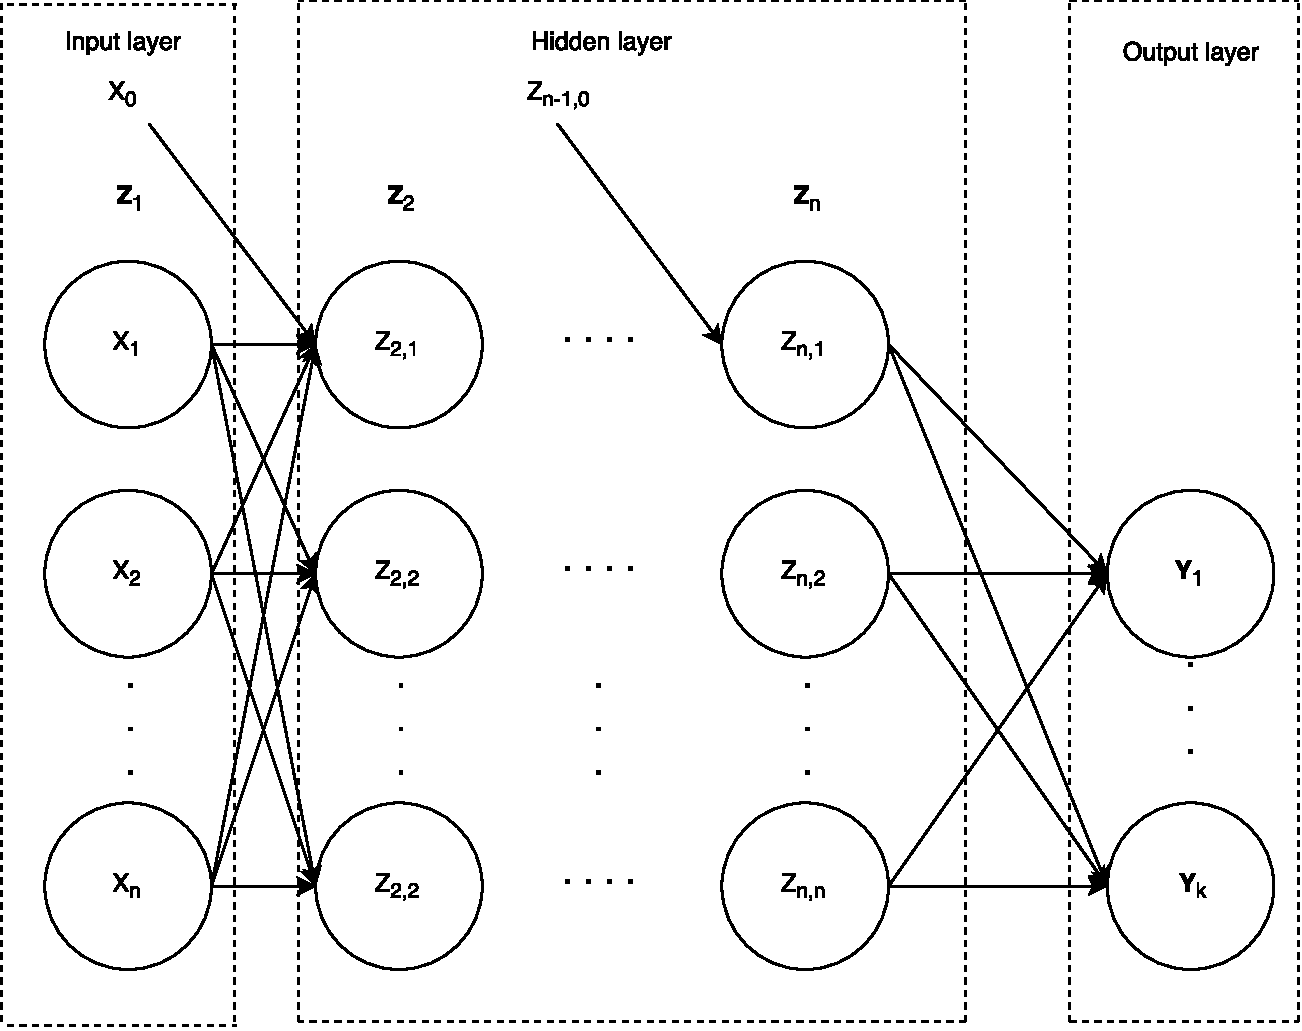
\includegraphics[width=0.8\textwidth]{report/figures/techniques/neural_network.pdf}
            \caption{A graph visualizing a N-level deep neural network. All hidden layers are fully connected. The size of the input and output layer depends on input size, and if the NN is used for regression or classification.}
            \label{fig:nn_fullnetwork}
        \end{figure}
        
        An NN is an n-class classification or regression algorithm. For anomaly detection, an NN can be trained to recreate the input of normal data. If the network is trained with enough normal data, it should be able to learn a good representation of patterns in this data. Abnormal data will in some way deviate from normal data, and hence its patterns are not familiar to the network. This will then result in recreated data that deviate more than normal from the input. This is also known as autoencoding. There are many types of NN specialized in solving specific tasks. Recurrent neural networks (RNN) are designed to learn trends seen over a period and are therefore a good option when working with time series. Within the recurrent NN, there is a type known as LSTM or long short-term memory, which has shown to outperform the standard RNN when it comes to long-horizon trends, \cite{Courville2016}. The following section introduces LSTM RNN by first introducing NN and RNN.  
        
        A visual representation of an NN is a graph with nodes and vertices as shown in Figure \ref{fig:nn_fullnetwork}. As seen, an NN consists of three parts, an input layer, a hidden layer, and an output layer. The input layer is the feature vectors for the data samples, the hidden layer does all the computation, and the output layer makes the prediction. An NN with only one layer and a limited number of neurons can approximate any function, \cite{Hastie}. This shows the ability an NN has for finding complex non-linear patterns.
        
        
        \begin{figure}[h]
            \centering
            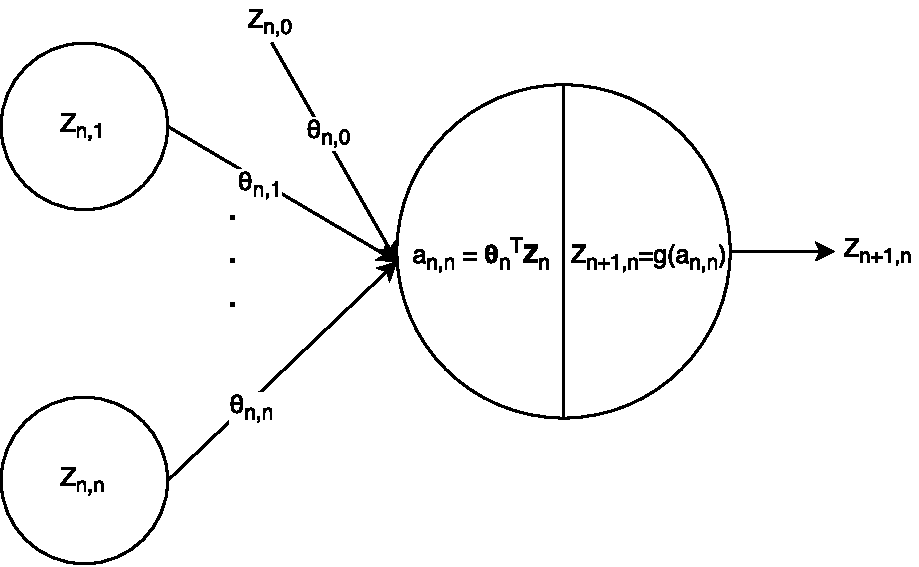
\includegraphics[width=0.5\textwidth]{report/figures/techniques/single_neuron.pdf}
            \caption{Visualization of a single neuron. The input is the output from the previous layer. The output is a scalar decided by the activation function $g(a)$}
            \label{fig:nn_neuron}
        \end{figure}
        
        Each of the nodes marked  $z_{n,n}$ seen in Figure \ref{fig:nn_fullnetwork} is known as a neuron. A single neuron is visualized in Figure \ref{fig:nn_neuron}. Each neuron does two things. First, it takes the dot product of the input vector and the weight vector, 
        
        \begin{equation}
            a = \bm \theta_n^T \bm Z_n,
            \label{eq:neuron_a}
        \end{equation}
        also shown in Figure \ref{fig:nn_neuron}. Then the output $Z_{n+1,n}$ is calculated 
        \begin{equation}
            Z_{n+1,n} = g(a_{n,n}).
            \label{eq:nn_activation}
        \end{equation}
        Here $g(a)$ is known as an activation function. There are many different options for activation functions, the most common are shown in Table \ref{tab:acitvations}. It is by using nonlinear activation functions, that a NN is enabled to approximate any function. If only linear functions are used, it can be verified that adding more layers does not but complicating a linear interpretation, \cite{Hastie}. The algorithm learns by updating the weights $\theta$ in each neuron.  
        
        
        %%%%%%%%% activation fucntions 
        % \begin{align}
        %     g_k(a) = a \textit{ identity function} \\
        %     g_k(a) = \frac{1}{1+e^{-a}} \textit{ sigmoid function} \\
        %     g_{k}(a) = \frac{e^{Tk}}{\sum_{i=1}^Ke^{Ti}} \textit{ softmax function} \\
        %     g_{k}(a) = \frac{e^a-e^{-a}}{e^a+e^{-a}} \textit{ tanh function} \\
        %     g_{k}(a) = max(a,0) \textit{ relu function}
        %     \label{eg:activations}
        % \end{align}
        
    \begin{table}[h]
        \centering
        \begin{tabular}{l l}
            \toprule
            \textbf{Function} & \\ \midrule
            Identity & $g_k(a) =a$ \\ 
            Sigmoid & $g_k(a) =\frac{1}{1+e^{-a}}$ \\ 
            Softmax & $g_k(a) =\frac{e^{Tk}}{\sum_{i=1}^Ke^{Ti}}$ \\ 
            Tanh & $g_k(a) =\frac{e^a-e^{-a}}{e^a+e^{-a}}$ \\ 
            Relu & $g_k(a) =max(a,0)$ \\ \bottomrule
        \end{tabular}
        \caption{Different activation functions}
        \label{tab:acitvations}
    \end{table}
        % \begin{align}
        %     z_{m} =  \sigma(\theta_{0m} + \bm \theta_m^T \bm z_{m-1}), \textit{m = 1,..,M} \nonumber \\
        %     \bm \hat y = g(\bm z_m) \nonumber \\
        %     \label{eq:fwdprop} 
        %     % \textit{where $\sigma()$ and g() are different activation function}\nonumber 
        % \end{align}
        % In the first layer, $\bm z_1 = \bm x$. For all the other layers each $z_m$ is given by the activations function of a bias term pluss the dot product of the inputs $\bm z$ and the weight $\bm \theta$. This means that for each layer there exists $m$ $\bm \theta$ vectors, which can be written as $\bm \Theta_m$. For the regression classifiers one only had one vector $\bm \theta$, but for a NN you end up with $m$ $\bm \Theta$ matrices. This gives a good indication on why a NN can approximate any given function. 
        The final layer calculates the output $\hat y$. The number of elements in the final layer depends as mentioned if it is classification or regression. For regression, the final layer usually only has one element, but for classification, it holds as many elements as there are classes. For binary classification, the Sigmoid function is typically used. For k-class classification, the Softmax function is used, and for regression the identity function.
        
        The weights of an NN are updated through forward and backward propagation. Forward propagation the input is fed through the mathematical operations in the network as seen in Figure \ref{fig:nn_neuron} and \ref{fig:nn_fullnetwork} and a set of labels or values are predicted. The cost function 
        \begin{align}
            E(\bm\Theta) = &\sum_{i=1}^M\frac{1}{2}(\hat{y} - y)^2 \nonumber,
            \label{nn:cost}
        \end{align}
        expresses how well the NN is able to correctly predict its output. The NN weights or coefficients $\bm \Theta = [\bm \Theta_1 ... \bm \Theta_n]$ are then updated through a step called backpropagation. The cost function is minimized as a function of the weigths. Gradient descent or another optimization algorithm is used to calculate each of the different parameters in $\bm \Theta$'s contribution to the cost. $\bm \Theta$ is updated as 
        \begin{align}
            \bm \Theta := & \bm \Theta - \alpha \nabla E(\bm \Theta) \nonumber \\
            \Theta_{ij} = & \Theta_{ij} - \alpha \sum_{k=1}^M \frac{\partial E_k}{\partial \Theta_{ij}} 
            \label{bp:1}
        \end{align}
        Here $\alpha$ is the learning rate, a value between [0,1]. The prediction errors are back-propagated to calculate the error in each neurons prediction. This prediction error is then used to update the corresponding weights for the neuron in the matrix $\bm \Theta$. A full mathematical proof can be found in \cite{Aasnes2017}
        
        % % Equation \ref{bp:1} to \ref{bp:9} shows how the partial derivative of the cost function is computed.   
        
        % \begin{align}
        %     \frac{\partial E}{\partial \Theta_{ji}} = \frac{\partial E}{\partial a_{ji}} \frac{\partial a_{ji}}{\partial \Theta_{ji}} \label{bp:2}.
        % \end{align}
        % Solving for the first term,
        % \begin{align}
        %     \delta_{ji} \coloneqq \frac{\partial E}{\partial a_{j,i}} = \sum_{k=1}^N \frac{\partial E}{\partial a_{j+1,k}} \frac{\partial a_{j+1,k}}{\partial a_{ji}} \label{bp:3}
        % \end{align}
        % where
        % \begin{align}
        %      \frac{\partial E}{\partial a_{j+1,k}} = \delta_{j+1,k}
        % \end{align}
        % and
        % \begin{align}
        %     \frac{\partial a_{j+1,k}}{\partial a_{ji}} = \frac{\partial \bm \theta_{j+1}^T \bm Z_{j+1}}{\partial a_{ji}}. \label{bp:4}
        % \end{align}
        % $\bm \theta_{j+1}^T \bm Z_{j+1}$ can be written as, 
        % \begin{align*}
        %     \bm \theta_{j+1}^T \bm Z_{j+1} = \Theta_{j+1,0}Z_{j+1,0} +\textit{ }..+ \textit{ }\Theta_{j+1,N}Z_{j+1,N} \nonumber \\
        %     = \Theta_{j+1,0}g(a_{j,0}) + \textit{ }.. +\textit{ }\Theta_{j+1,N}g(a_{j,N}). \label{bp:5}
        % \end{align*}
        % This gives, 
        % \begin{align}
        %     \frac{\partial a_{j+1,k}}{\partial a_{ji}} = \Theta_{j+1,i}\frac{\partial g(a_{j,i})}{\partial a_{ji}} =  \Theta_{j+1,i}g'(a_{ji}), \label{bp:6} 
        % \end{align}
        % which finally yields
        % \begin{align}
        %     \delta_{ji} = g'(a_{ji})\sum_{k=1}^N\delta_{j+1,k}\Theta_{j,k}. \label{bp:7}
        % \end{align}                    
        % Solving for the second term
        % \begin{align}
        %     a_{ji} = \bm \theta^T_i \bm Z_{i} \label{bp:10}
        % \end{align}
        % \begin{align}
        %     \frac{\partial a_{ji}}{\partial \Theta_{ij}} =  Z_{ji} \label{bp:8}
        % \end{align}
        % Gives the following equation
        % \begin{align}
        %     \frac{\partial E}{\partial \Theta_{ji}} = \delta_{ji}Z_{ji} \label{bp:9}
        % \end{align}
        
        The forward and backward-propagation steps are then iterated over until a given number of iterations are reached. A complete pass forward and backward of all training examples are known as one epoch. When the training set is large, it is often split into smaller batches to speed up calculations. The batch size explains how many samples are included in each forward and backward pass. Splitting the data into batches enables the algorithm to take advantage of parallelism, running the separate batches on separate CPUs or GPU's. How many epochs it takes for an NN to learn a good representation of the data can vary a lot. A technique called early stopping is introduced to ensure that the NN is stopped when the network no longer is showing sign of increased test predictions. Running an NN for too many epochs on a training set can cause the NN to overfit to the training data, giving poorer general performance than if stopped earlier.  
        
        
        A deep NN can learn more complex patterns than a shallow. However, the deeper the NN is, the more processing each iteration through it will take. Deep networks also increases the risk of overfitting. A good approach is to start with a shallow network, and increase the depth and width until you see that adding new layers, does not yield better performance. Other means to handle overfitting is regularization (making it costly to have large weights) and dropout. Dropout removes some edges between the neurons between each iteration, simplifying the network structure. 
        % To avoid overfitting the regularization term 
        % \begin{align}
        %     \frac{\lambda}{2} \sum_{km} \Theta_{km}^2  \nonumber \\
        %     = \frac{\lambda}{2}\bm \Theta^T \bm \Theta,
        %     \label{nn:overfit}
        % \end{align} 
        % is added to the cost function. The extra term in the cost function will penalize parameters $\neq 0$. This slightly modifies the update rule as 
        % \begin{align}
        %     \bm \Theta = & \bm \Theta - \alpha \nabla E(\bm \Theta) - \alpha \frac{\lambda}{2} \frac{\partial \bm \Theta^T \bm \Theta}{\partial \bm \Theta} \nonumber \\
        %     = &(1-\alpha \lambda)\bm \Theta - \alpha \frac{\partial E(\bm \Theta)}{\partial \bm \Theta}.
        %     \label{nn:updaterule2}
        % \end{align}
        % Since the regularization term is introduced to reduce the weights in the NN, it is a natural conclusion that the weights should be initialized to small values. Zero initialization is however not a good option, this will lead to zero derivatives, and hence the model will never be updated. Initializing all weights to a random number near zero, will give a roughly linear model \cite{Hastie}. This means that the model will start out more or less as a linear function and will grown in nonlinearity if necessary.
    
    
    \subsection{Recurrent neural network}\label{subsubsec:RNN}
        Recurrent NN is a type of NN designed for sequential data. The RNN is specialized for processing values that belong to a sequence, as often is the case with time-series data. It is designed to scale to much longer sequences than what is practical for standard fully connected NN. The key is parameter sharing, which enables one to apply a model to different sequence lengths and generalize across them. The following quote from \cite{Courville2016} explains this well. "For example, consider the two sentences “I went to Nepal in 2009” and “In 2009, I went to Nepal.” If we ask a machine learning model to read each sentence and extract the year in which the narrator went to Nepal, we would like it to recognize the year 2009 as the relevant piece of information, whether it appears in the sixth word or in the second word of the sentence. Suppose that we trained a feedforward network that processes sentences of fixed length. A traditional fully connected feedforward network would have separate parameters for each input feature, so it would need to learn all the rules of the language separately at each position in the sentence. By comparison, a recurrent NN shares the same weights across several time steps". Figure \ref{fig:RNN} shows a representation of a RNN. The RNN can be unfolded into a set of networks for a finite number of time steps as shown in the right of Figure \ref{fig:RNN}, once the network is unfolded in this way the backpropagation can be computed, as explained in the above section. The internal state of the NN is updated as
        \begin{align}
            c^{(t)} = f(c^{(t-1)},x^t;\theta), 
            \label{eq:RNN}
        \end{align}
        here it becomes apparent that the current state is dependent on the previous state, which again is dependent on its predecessor, and so on. This clearly shows the recurrent pattern. 
        
        
        \begin{figure}
            \centering
            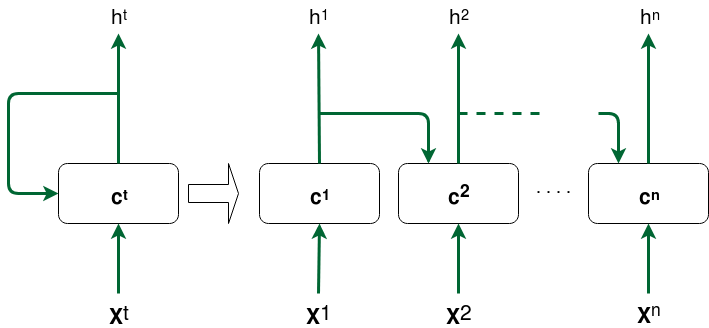
\includegraphics[width=\textwidth]{report/figures/techniques/RNN.png}
            \caption{A recurrent neural network, shown in its compact form to the left, and in its unrolled form to the right.}
            \label{fig:RNN}
        \end{figure}
    
        One of the downfalls of the RNN is that as the depth of the network grows with the number of time steps. This introduces two problems known as vanishing and exploding gradient. This phenomenon is explained in detail in \cite{Pascanu}. The short version is that as the number of time steps grows, the size of the network grows. This means that the number of computations in the backpropagation algorithm also grows. It can be shown that each of the n layers as seen in Figure \ref{fig:RNN} gets its parameters updated as a partial derivative of the cost function for its prediction, in addition to the partial derivative of the next network. The exploding or vanishing gradient problem can be found by examining how $\frac{\partial \bm x_t}{\partial \bm x_k}$ is calculated. The following derivation from \cite{Pascanu},
        \begin{align}
            \frac{\partial \mathcal{E}}{\partial \theta} = \sum_{1\leq k \leq t}\frac{\partial \mathcal{E}_t}{\partial \theta} \nonumber \\
            \frac{\partial \mathcal{E}_t} = \sum_{1\leq k \leq t}\frac{\partial \mathcal{E}_t}{\partial \bm{x_t}} \frac{\partial \bm{x_t}}{\partial \bm{x_k}}\frac{\partial \bm{x_k}}{\partial \theta} \nonumber \\
            \frac{\partial \bm{x_t}}{\partial \bm{x_k}} = \prod_{t \geq i\geq k} \frac{\partial \bm{x_i}}{\partial \bm{x_{i-1}}}\label{eq:rnn_xprod}, 
        \end{align}
        shows how the partial is calculated. As seen in Equation \ref{eq:rnn_xprod} the partial of $\bm x_t$ becomes a product of all internal states of the timesteps between t and k. Hence, if these values are $\geq1$ the gradient will grow, and if they are $\leq 1$ they will decrease. As the number of timesteps grows, the gradient then runs the risk of either explode or vanish. A possible solution to this problem is presented in the next section.  
    
    \subsection{Long short term memory recurrent neural networks}
        Long Short-Term Memory RNN or LSTM RNN is an extension of the RNN seen in subsection \ref{subsubsec:RNN}. The idea behind it is to create loops where the gradient can flow for long durations, and hence solving the issue with vanishing and exploding gradients. LSTM was introduced in \cite{Hochreiter1997}, and has been found very successful in many different applications. Figure  \ref{fig:lstm} shows the building blocks of the LSTM. The LSTM consist of four internal layers, forget layer, input gate layer, two tanh layers and the output layer. All of those layers are a separate NN layer. The previous cell state is fed in at the top of the LSTM. The previous state is kept based on the previous output $\bm h^{t-1}$ and the current input $\bm x^t$ which is fed through the forget layer. If none of the previous states is seen as relevant, the output will be a vector of zeros. If the previous state is seen as extremely important, it will output a vector of ones. Next, the information in the new input is analyzed. The tanh layer creates an estimation of the current LSTM state $\bm c^t$ based on $\bm h^{t-1}$ and $\bm x^t$. This value is then scaled by the output of a sigmoid layer $\bm I^t$ which decides which of the internal states to update. $\bm c^t$ is then computed as a function of the previous state and the new state estimation. The output is calculated by sending the current cell state through a tanh layer before a sigmoid layer decides which part of the cell state to output.  
        
        \begin{figure}
            \begin{minipage}[b]{0.99\linewidth}
            \centering
            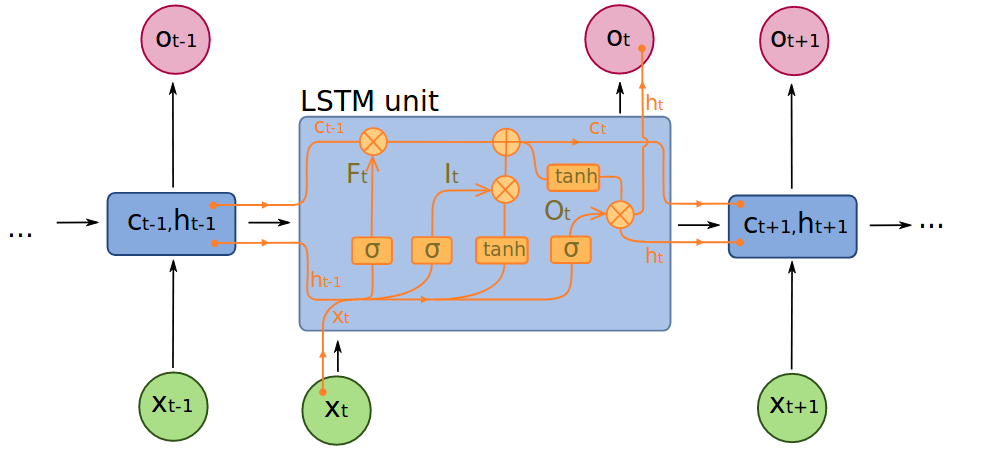
\includegraphics[width = \textwidth]{report/figures/techniques/lstm.png}
            \caption{A lstm network, By François Deloche \footnote{Lisenced under CC BY-SA 4.0, \url{https://commons.wikimedia.org/wiki/File:Long_Short-Term_Memory.svg}}} 
            \label{fig:lstm}
            \end{minipage}
        \end{figure}
        
        
        LSTM is proposed as a scheme for anomaly detection in \cite{Malhotra2016} and \cite{Malhotra}. It is shown that the scheme is working for both periodic and aperiodic time series. LSTM RNN has been successfully used for handwritten text recognition and speech recognition. The paper proposes an encoder-decoder scheme designed for anomaly detection. A time series is encoded and then decoded back to reconstruct the input series. The reconstruction error, the error between the input and the reconstructed input is then used to identify outliers. In the training phase, the system is only shown normal data. Hence it only learns to reconstruct the normal system behavior. The network should then not be able to reconstruct anomalous data as good as with normal data. The paper concludes that LSTM networks can be a viable approach for anomaly detection. It also shows promise in detecting anomalies from unpredictable time-series.      
        
%!TEX root = ../Thesis.tex
\chapter{Implementation}\label{cha:implementation}
This chapter introduces the system implementation and the software packages used during the thesis.

\section{Python}
    All code is developed in Python 3.6 through Anaconda and Spyder. Anaconda is a Python distribution with focus on data science and machine learning. Anaconda simplifies installation and handling of packages and package dependencies. In addition, it allows exporting of the package environment, for automatic setup at new locations. Spyder is a Python IDE that has a similar layout to Matlab, where objects and variables can be accessed through a workspace. This makes it a good alternative for data science. 
    
    A library for reading and preparing the data from the energy company is created from scratch. The library is meant to be used for further analysis at Hymatek. The code used for OC SVM is mostly reused from the project thesis. All other code is written during the master thesis. All methods mentioned in theory is implemented and ready for use. Libraries are created that makes it easy to analyze the data on the different methods. The next subsections are taken from \cite{Aasnes2017} 
    
    
\section{Scikit-learn}
Scikit-learn, \cite{scikit-learn} and \cite{scikit-web} is an open source toolbox available for Python. It includes many different machine learning algorithms and the tools needed to preprocess and analyze data. The framework created by scikit-learn is used throughout this thesis, as it includes implementations of OC SVM and KDE. It also has implementations of many other machine learning algorithms, if one wants to expand the analysis with new methods. In addition to the being a great machine learning library for Python, the website \footnote{\url{http://scikit-learn.org/stable/ }}also explains the main theory behind the different algorithms, and what the scikit-learn algorithms are built upon in an easy to find manner. This makes it a good choice when one want to understand what is making the algorithms work.        

\section{Keras}
    Scikit-learn does not include neural networks. Different libraries were considered before Keras was chosen for the NN analysis. Keras \cite{chollet2015keras} is a Python library that simplifies creation of NNs in Python. Instead of having its own implementation of NNs, it uses other NN Python libraries as backends. This means that you can run the analysis using, for example, Google's TensorFlow through Keras. At this moment Keras supports Google's TensorFlow, Theano developed by LISA Lab at Université de Montréal and CNTK developed by Microsoft. This means that by using Keras, only one line of code needs to be changed if one want to change between one of the options above. Developing code using one of the NN libraries directly would make switching between the different options more cumbersome. However, one important factor to keep in mind, is that Keras is not officially supported by any of the backend developers. This means that  not all of the original functionality is guaranteed to be supported in Keras. Regardless, the fact that Keras is easy to use and its focus on enabling fast experimentation, are the main reasons for developing in Keras. Keras supports the many different types of NN, including the LSTM RNN used in this thesis. Keras also enables the user to choose to run on either CPU or GPU, making it flexible and easy to optimize to the available hardware. More information about Keras can be found at \footnote{\url{https://keras.io/}}.
        
    \subsubsection{Google TensorFlow}
        For this thesis, only the TensorFlow backend is used. TensorFlow \cite{Abadi} is developed by The Google Brain project, and it started as the DistBelif project back in 2011. Tensor flow is the second generation, built upon the experiences from DistBelif. Tensorflow has support for parallelism and can have many different devices collaborating on the same problem. As stated in \cite{Abadi}, "a computation expressed using TensorFlow can be executed with little or no change on a wide variety of heterogeneous systems, ranging from mobile devices such as phones and tablets up to large-scale distributed systems of hundreds of machines and thousands of computational devices such as GPU cards." This shows the flexibility TensorFlow introduces. More information about TensorFlow can be found at \footnote{\url{https://www.tensorflow.org/}}.
    
    
    
% \chapter{Analyzing the dataset and building a case}\label{cha:data}

This chapter introduces the dataset and work done to enable information extraction and analysis of the provided data. The case for the analysis is also introduced.


% In the data set, three power plants have Pelton turbines with measurement of their needle position. More information about a Pelton turbine can be found in chapter \ref{cha:data}. One of the power plants had recorded several issues with the control and behavior of the needles during operation. There were many interesting events spread out over many of the power plants, but one major benefit with the Pelton needle case was that there was one plant with several reported issues for the same component. In most of the other cases, there were only recorded one incident on one plant, making them hard to analyze and validate. The fact that there are two additional power plants with the same process signals without reported issues opened up the possibility for testing and validating the chosen techniques not only on data from the faulty plant. This also introduced the possibility to validate how well and how easy the different techniques could adapt to new plants.    




% Based on the arguments above, the Pelton needle case was chosen as the focus of the thesis. The following points were then defined as a basis for the analysis. 


\section{Dataset}\label{sec:dataset}
    Hymatek controls provided a dataset from a Norwegian energy company, containing process information from $27$ hydroelectric power plants logged from $2013$ to mid $2017$. The data is not pre-processed in any way, and come just as it is logged at the company. A big part of the thesis has been spent on exploring the data, finding out what is logged and what can be used. The data is split into five folders, one for each year. In each folder, several different files are stored. Table \ref{tab:data_files} shows the different file types that are found in the dataset. The file names indicated the frequency, sampling type and sampling duration of the data. The files are not separated by plants, only by date. Hence, a file containing data sampled every second for any given start and stop date contains data from all plants for that given period. In addition to the data files, a meta-data file is provided where plant name and process signal for each tag can be found.
    
    \begin{table}[]
        \centering
        \begin{tabular}{c c c c c}
        
        \toprule
             \textbf{Interval}   & \textbf{Average}   & \textbf{Max}   & \textbf{Min}   & \textbf{Actual}    \\ \midrule
             Daily      & x         & x     & x     & -         \\ 
             Hourly     & x         & x     & x     & -         \\ 
             Minutely   & x         & x     & x     & -         \\ 
             Secondly   & -         & -     & -     & x         \\ \bottomrule
        \end{tabular}
        \caption{Table showing the available data for the different sampling frequencies}
        \label{tab:data_files}
    \end{table}
    
    The total size of all files exceeded $90$Gb. This means that one can't merely load all data into the computer memory, and work with it from there. The information needs to be extracted one plant at a time, for each of the different sampling rates and stored in a way that enabled fast and efficient loading.

    
    \subsection{Old and new data format}\label{subsec:data_format}
        Regardless of sampling-rate and data type, the files are all in the same format. As seen in Table \ref{tab:orig_data}, each line holds a tag, a time of sampling and process value. 
        \begin{table}[h]
            \centering
            \begin{tabular}{c c c}
                \toprule
                 \textbf{Tag}        & \textbf{Timestamp}         & \textbf{Value}  \\ \midrule
                 192390514  & 20170101000000000 & 0.897244155 \\
                 192391514  & 20170101000000000 & -0.549806237 \\ \bottomrule
            \end{tabular}
            \caption{Example of the structure of the original datasets}
            \label{tab:orig_data}
        \end{table}
        Once a file is loaded the tag is replaced by the process-signal name found in the meta-data file. To enable interpretation and analysis of the data, it is decided that new datasets needs to be created on the format shown in Table \ref{tab:plant_format}.
        \begin{table}[h]
            \centering
            \begin{tabular}{c c c c c }
                \toprule
                \textbf{Time stamp} & \textbf{P. variable 1}     & \textbf{P. variable 2}    & \textbf{..}    & \textbf{P. variable n}    \\ \midrule
                time 1        & NaN         & $2$           & ..    & NaN         \\ 
                time 2        & $3.00$      & NaN           & ..    & $0.00214$\\ 
                :            & :            & :             & ..    & : \\ 
                time n        & $1.00$      & NaN           & ..    & $0.814$\\ \bottomrule
            \end{tabular}
            \caption{Example showing how the data looks for each plant after reconstruction is complete}
            \label{tab:plant_format}
        \end{table}

        
    \subsection{Overview of the datasets}
        Once the data is reconstructed as specified in subsection \ref{subsec:data_format} one can look into what information it holds. The number of available process signals varies a lot, from above $250$ to below $20$, as can be seen in Figure \ref{fig:process_signal_overview}. This was used as a first stage filtering to reduce the number of plants to examine. The plants with fewer than $30$ process-signals are dropped from the analysis, reducing the number of plants in the dataset to $15$.    
        
        \begin{figure}[h]
            \centering
            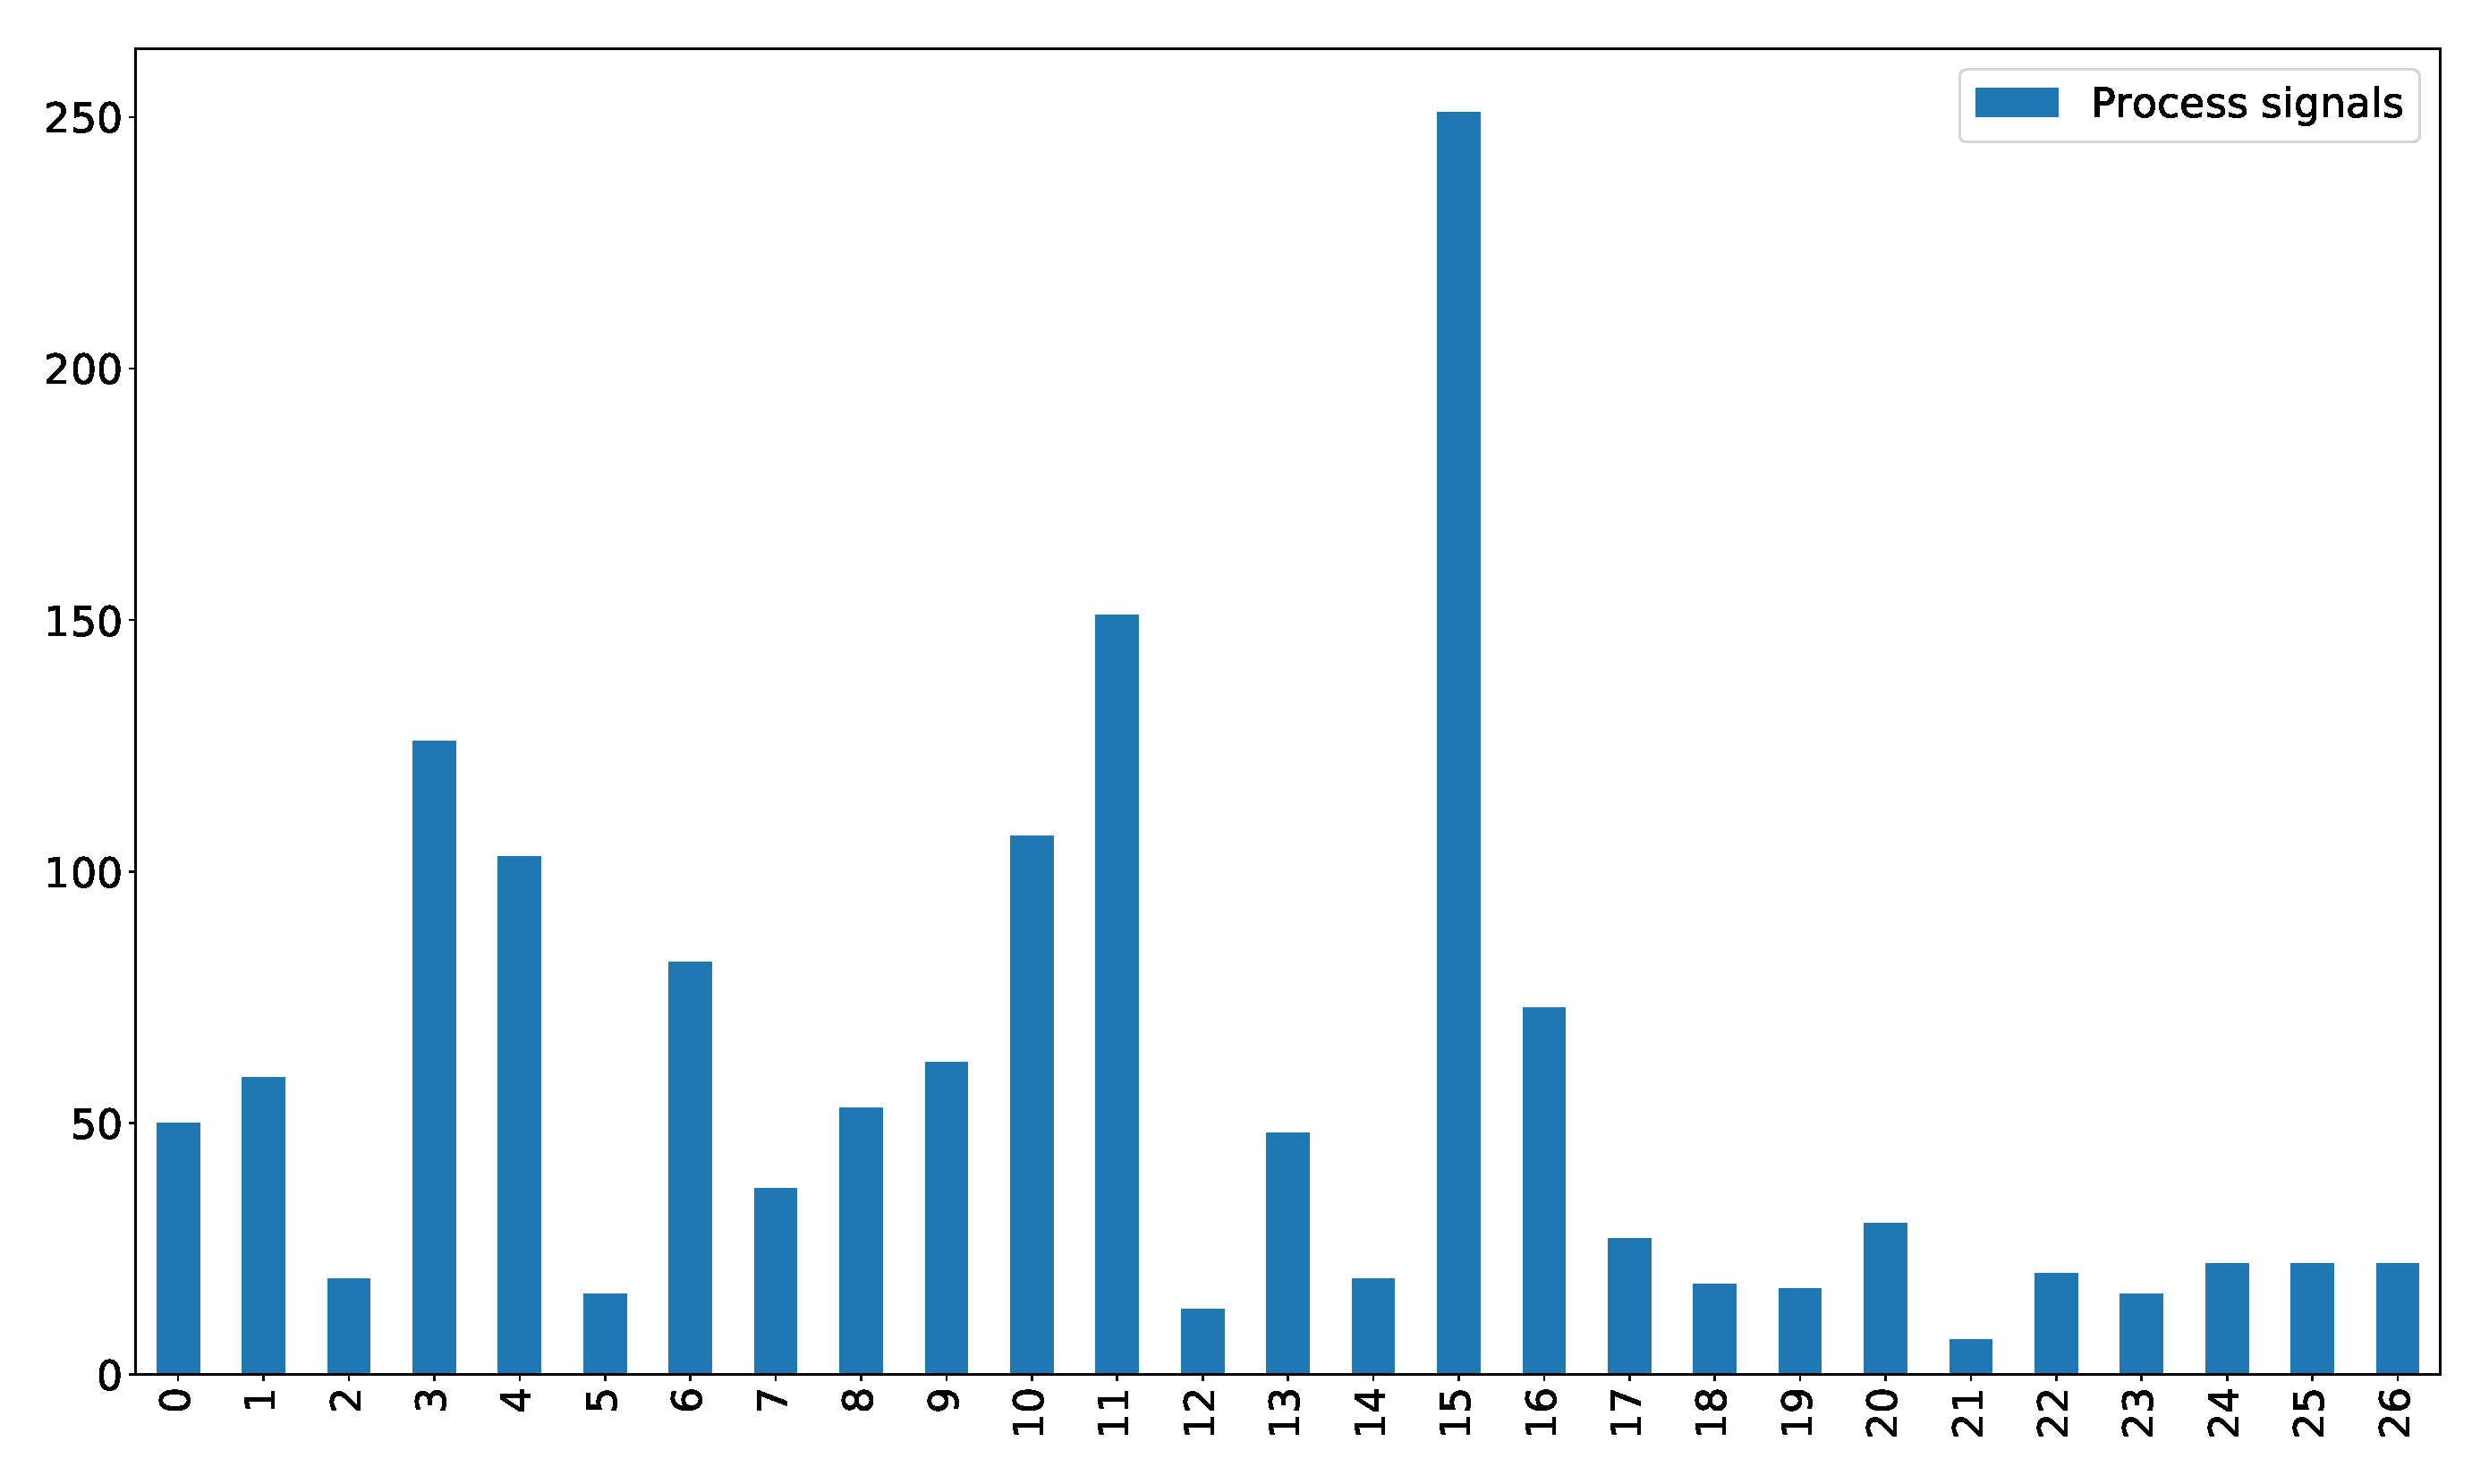
\includegraphics[width=\textwidth]{report/figures/data/plant_process_signals_overview.pdf}
            \caption{Overview of the number of process-signals or features for each of the 27 plants in the dataset.}
            \label{fig:process_signal_overview}
        \end{figure}
        
        After discarding the plants with few signals, the type of process-signals available is looked into. The more data sampled from different parts of a plant, the better. Having data from several parts and components of a plant can enable finding a link between unknown components and sensors. Figure \ref{fig:signal_type_overview} shows the different types of signals found in the datasets for the different plants. As can be seen, the temperature is one of the most common signals for all plants. There are also many signals of type "Def Type Måling", which is a common name that covers all signals not defined with a unique tag. Pressure, level, vibration, and so on are signals covered by this tag. Since all of the remaining plants has process-variables of different types, none are removed. 
        
        \begin{figure}
            \centering
            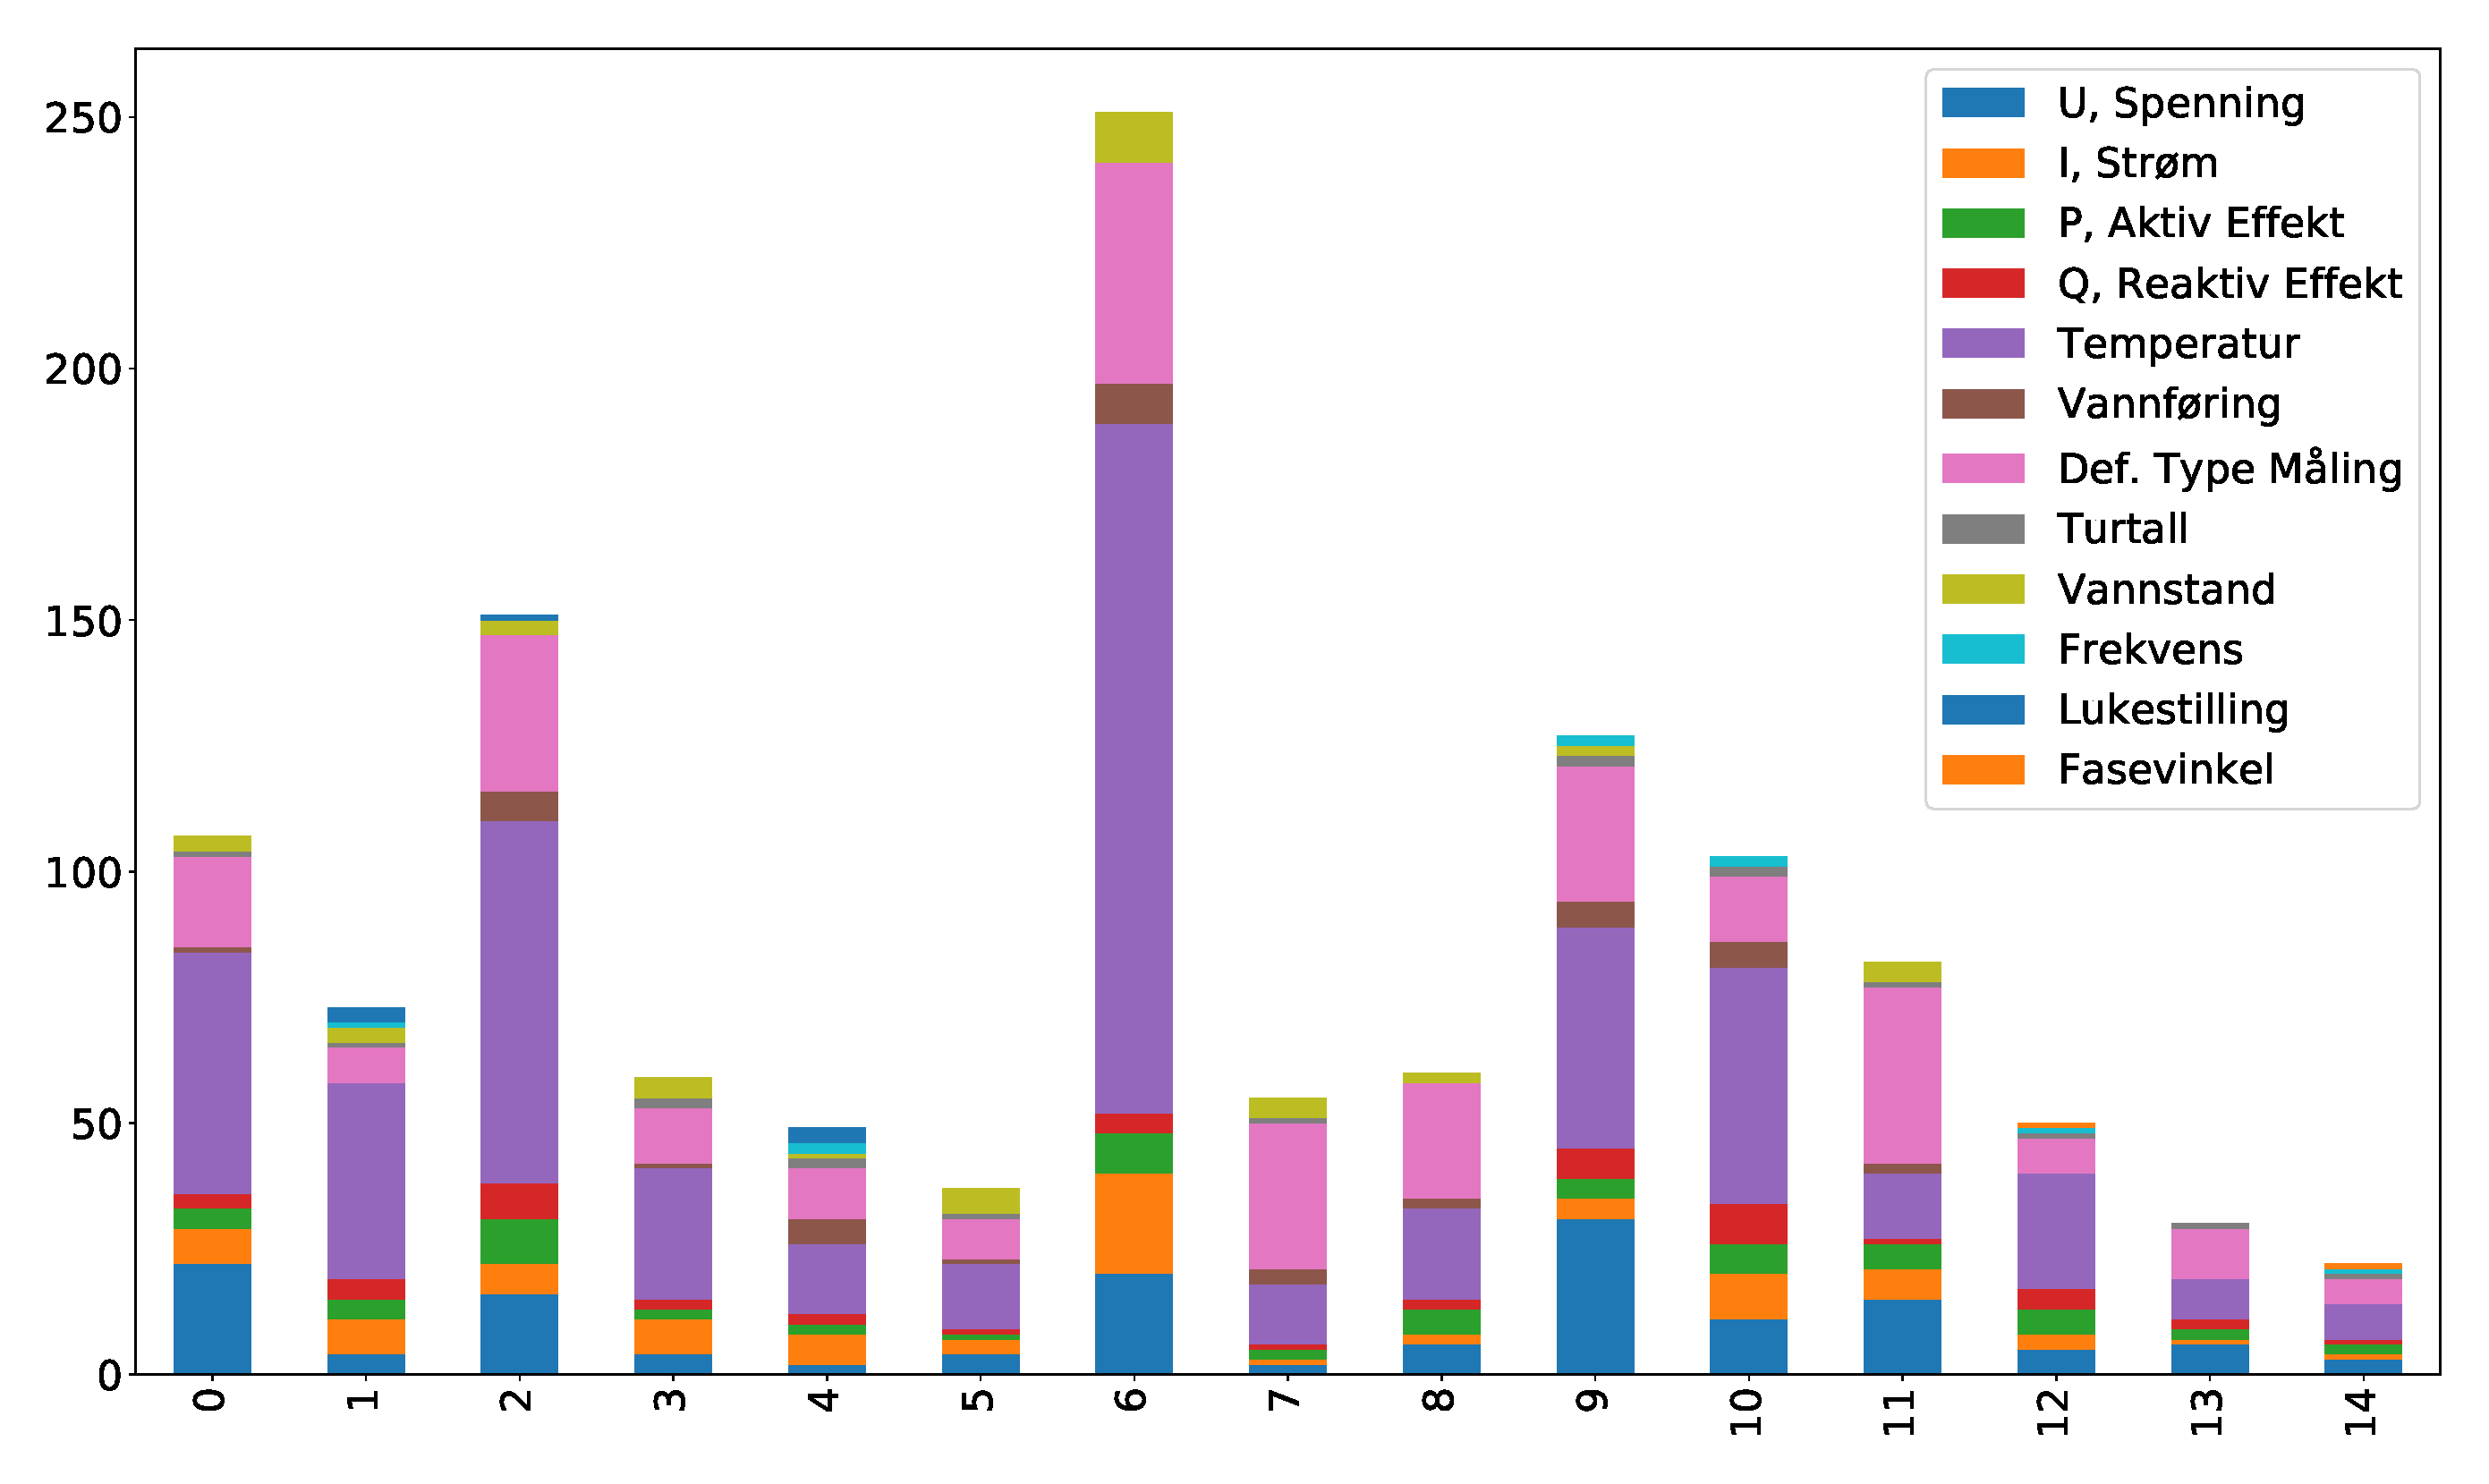
\includegraphics[width=\textwidth]{report/figures/data/plant_signal_types_overview.pdf}
            \caption{Figure showing the different process signals or features found at each of the 27 plants in the dataset.}
            \label{fig:signal_type_overview}
        \end{figure}
        
        % It is only necessary to keep the datasets with the highest sampling rate. The highest sampling rate will provide the most detail about a plant, and lower sampling rates can always be extracted from higher rates.
        
        % was decided to only use the datasets sampled every second. Using these datasets gave a snapshot of the plant state at a given time. Pandas have a lot of built-in functionality that enables easy re-sampling so that the average, max and min datasets could easily be recreated from this dataset if wanted.
        
        An issue arose when looking in detail at the datasets. Preferably, all process-signals should be sampled periodically and at the same time. This is however not the case, only at hourly resolution are the data matrices complete. At higher sampling rates there are a lot of missing data. At the highest sampling frequency (every second), there are many time-stamps where none of the process signals are sampled, and those that are sampled, often only samples one process-signal. This means that one either has to work with only hourly sample rate, work with incomplete datasets or reduce the number of process signals to investigate. Either the equipment used for sampling is not working as it should, or the varying sampling rate must be on purpose. It could be that a similar sampling scheme to the one seen in \cite{Selak2014} is used. This is however not possible to confirm from the data alone, and the energy company did not provide this information. This sheds light on the fact that having lots of data is not always a sign of quality. The data sampled in $2013$ is poorer than the later years, and hence it is dropped from any further analysis. 
    % \subsection{Instrumentation}\label{subsec:instrumentation}
    %     what is there of instrumentation? refer to the data I have gotten         
        
    \subsection{The historical log of the plants }
        Once an overview of the data was in place, the energy company was contacted, requesting an incident log from the remaining plants. Incident logs for the entire sampling period, for all of the $27$ power plants, were received. The level of details in the logged incidents is very varying from plant to plant. Some plants have reported over 200 incidents, while others barely exceeded 20. Many of the incidents are also minor incidents like a broken light bulb or nonfunctioning tools. Finding interesting incidents was time-consuming. Several interesting incidents were found, but very few were reported to occur more than once. Having few incidents makes it hard to separate valuable information from noise. Only having a limited number of faults can easily lead to overfitting. There is always a risk that randomness can cause the correlations and variable dependencies found. This needs to be taken into consideration when working such cases.  
        
        In the log for one of the power plants, it was found an error with the needles for a Pelton turbine. The error reported that as the opening of needle four of turbine two decreased below $46\%$, it started to lag behind needle two. The plant has two turbines that both have four needles. A search through the $14$ remaining power plants showed that there are two additional plants with Pelton turbines. These plants have however not reported any problems with the Pelton needles. This could then be a possible reference for normal operation. Also, it opens the possibility for testing how adaptable the anomaly detection methods are. 
        
        % \todo{remove this or add more analysis}When looking into the historical log of the plant, it was found that several more incidents with the Pelton needles were reported for the two turbines
        
\section{Pelton needles case}\label{sec:pelton_needles}
    The Pelton needle case was chosen for further analysis for several reasons. Firstly it is a critical part of the Pelton turbine, if the needles are not operating as they should it will affect the power produced by the turbine. The needle openings are a big part of a complex control system, that controls that the turbine holds constant speed. Finding a method that can give early warnings about incidents like the one above, means maintenance can be planned, and components overhauled before the system condition becomes too severe. Secondly, having data from different plants makes it possible to analyze how well the methods and techniques used to adapt to new data. This is an important factor, if one can develop a method that is transferable with little to no adaptation need between plants, the time for commissioning will be significantly reduced. In addition, this case fits well as an extension of \cite{Aasnes2017}, where the condition of the guide vanes for a Francis turbine was analyzed. Finally, quality and available process variables vary a lot from plant to plant. One of the most significant issues was that the majority of the process signals were not sampled at a constant frequency. The Pelton needles were found to be sampled in a manner that allowed the use of data from two separate plants.
             

    \subsection{Pelton needle incident 02.03.2017}
        As the incident reported that one needle was lagging behind another, it could indicate pairwise operated needles. This can also be justified from a practical perspective if the needles are placed opposite of each other they will give the turbine an even momentum as long as they lead the same amount of water onto the turbine. To confirm this, scatter-plots were created where each needle is plotted against the other. To enable this the needle process signals are pairwise extracted from the rest of the dataset, and all time-stamps where both needles are not sampled are removed. Figure \ref{fig:plant1_needles} shows the scatter-plot of the pairwise operated needles for both turbines at plant 1. As can be seen in all four plots, the majority of the data follows a linear dependency between the needles. However, several data-points deviate from this, especially for needle pair $[2,4]$ on turbine $2$, which had the reported incident. The plot in the bottom right corner shows what appears to be operational problems. It is only needle [1,3] on turbine 1 seen in the upper left plot, which follows the linear pattern.
        \begin{figure}
            \begin{minipage}[b]{0.5\linewidth}
                \centering
                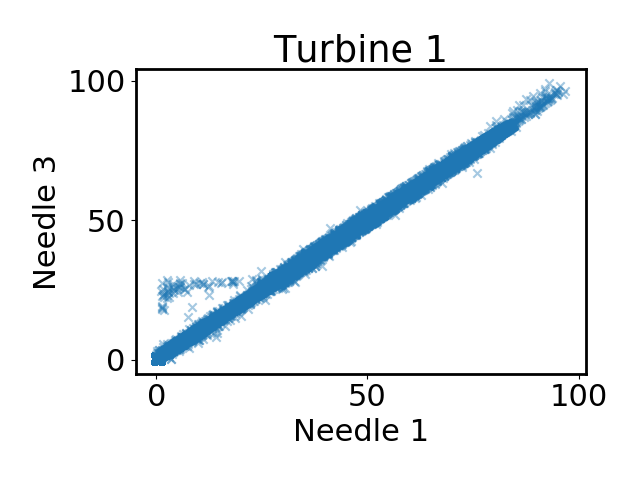
\includegraphics[width=\textwidth]{report/figures/data/t1_n1_n3.png}
            \end{minipage}
            \begin{minipage}[b]{0.5\linewidth}
                \centering
                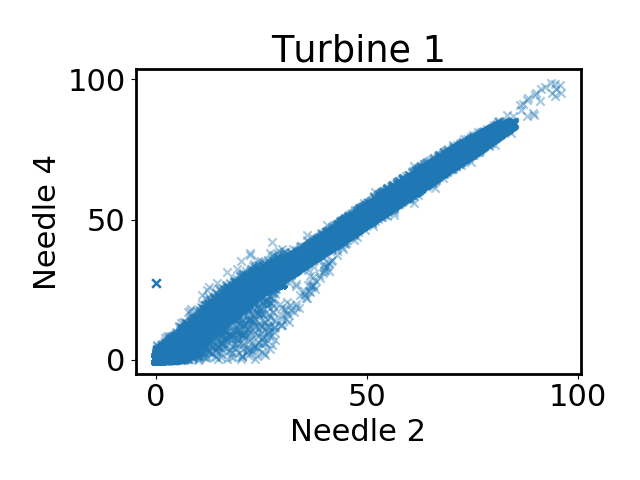
\includegraphics[width=\textwidth]{report/figures/data/t1_n2_n4.png}
            \end{minipage}
            \begin{minipage}[b]{0.5\linewidth}
                \centering
                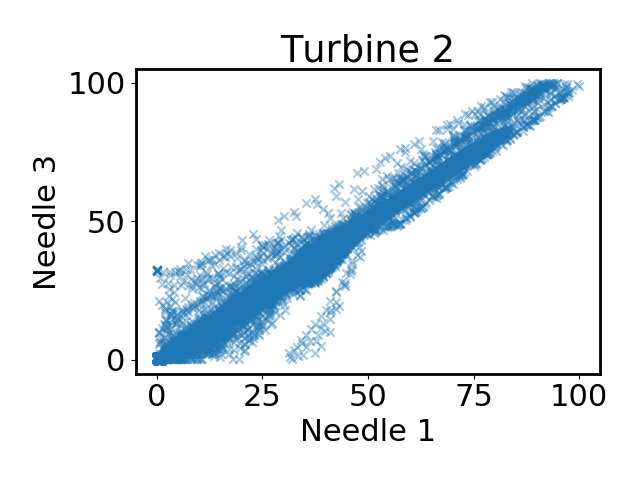
\includegraphics[width=\textwidth]{report/figures/data/t2_n1_n3.png}
            \end{minipage}
            \begin{minipage}[b]{0.5\linewidth}
                \centering
                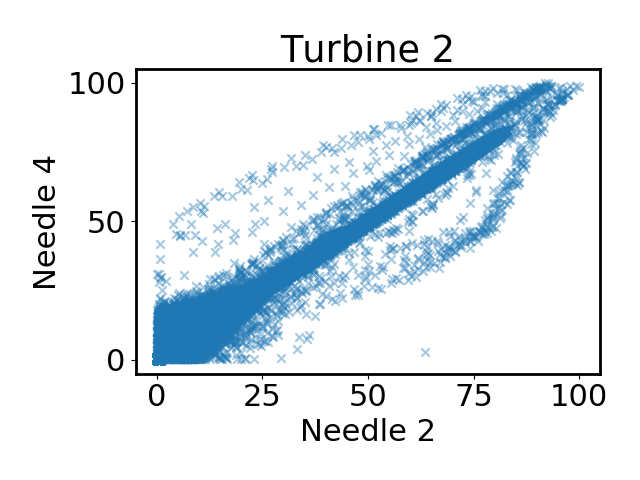
\includegraphics[width=\textwidth]{report/figures/data/t2_n2_n4.png}
            \end{minipage}
            \caption{Needle openings for the pairwise operated needles for both turbines at Plant 1 are scatterplotted in four sub-figures.}
            \label{fig:plant1_needles}
        \end{figure}
        
        % \begin{figure}[h]
        %     \centering
        %     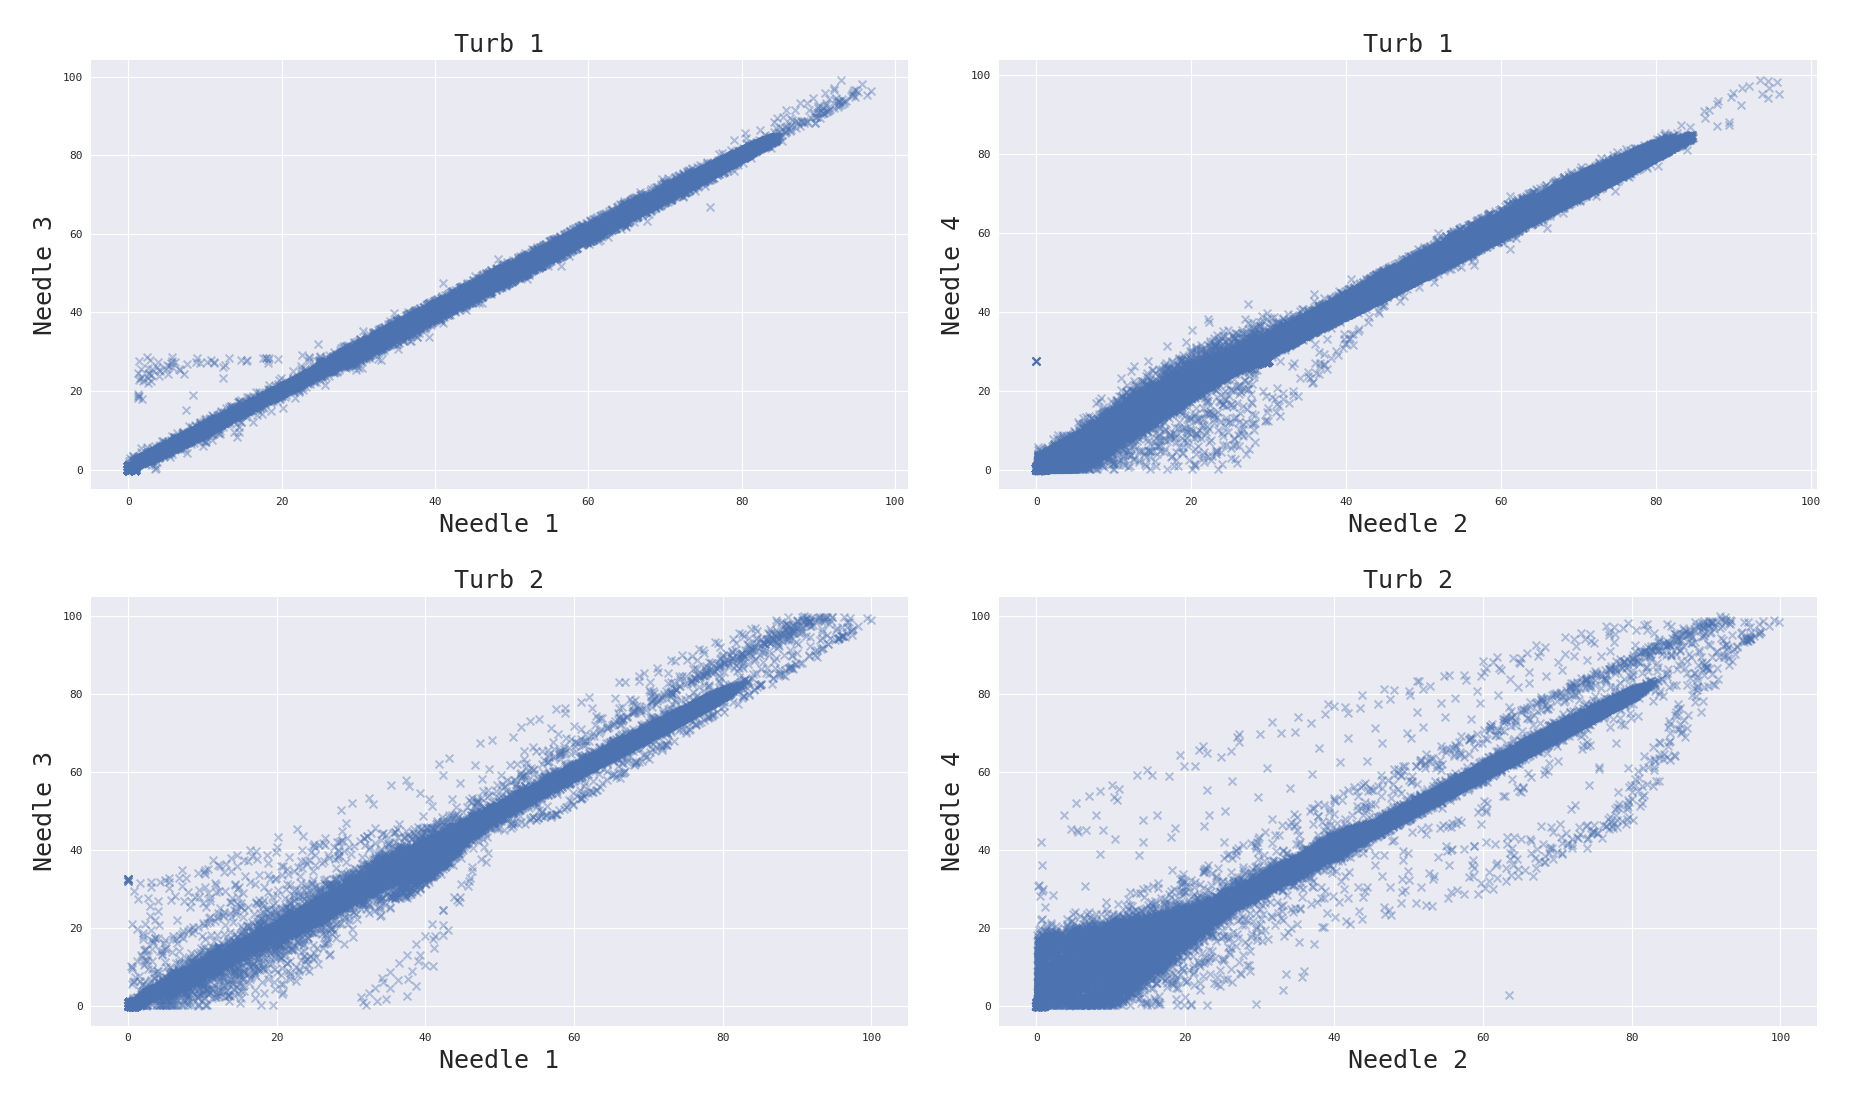
\includegraphics[width=\textwidth]{report/figures/data/plant1_needles.png}
        %     \caption{Pairwise operated needles for the two turbines at Plant 1 are scatterplotted in four subfigures. }
        %     \label{fig:plant1_needles}
        % \end{figure}
        % Figure \ref{fig:n_pos_0203} to \ref{fig:n_pos_aft_0303} shows the needle positions for two dates surrounding the reported incident, and all data after. Figure \ref{fig:n_pos_aft_0303} show that the problem was fixed when reported in early March. Figure \ref{fig:n_pos_0203} and \ref{fig:n_pos_0303} shows the two days with worst performance, and one can see that many of the worst data-points from the lower right plot in figure \ref{fig:plant1_needles}, looks to be the same as the ones shown in figure \ref{fig:n_pos_0203} and \ref{fig:n_pos_0303}.
        \begin{figure}
            \centering
            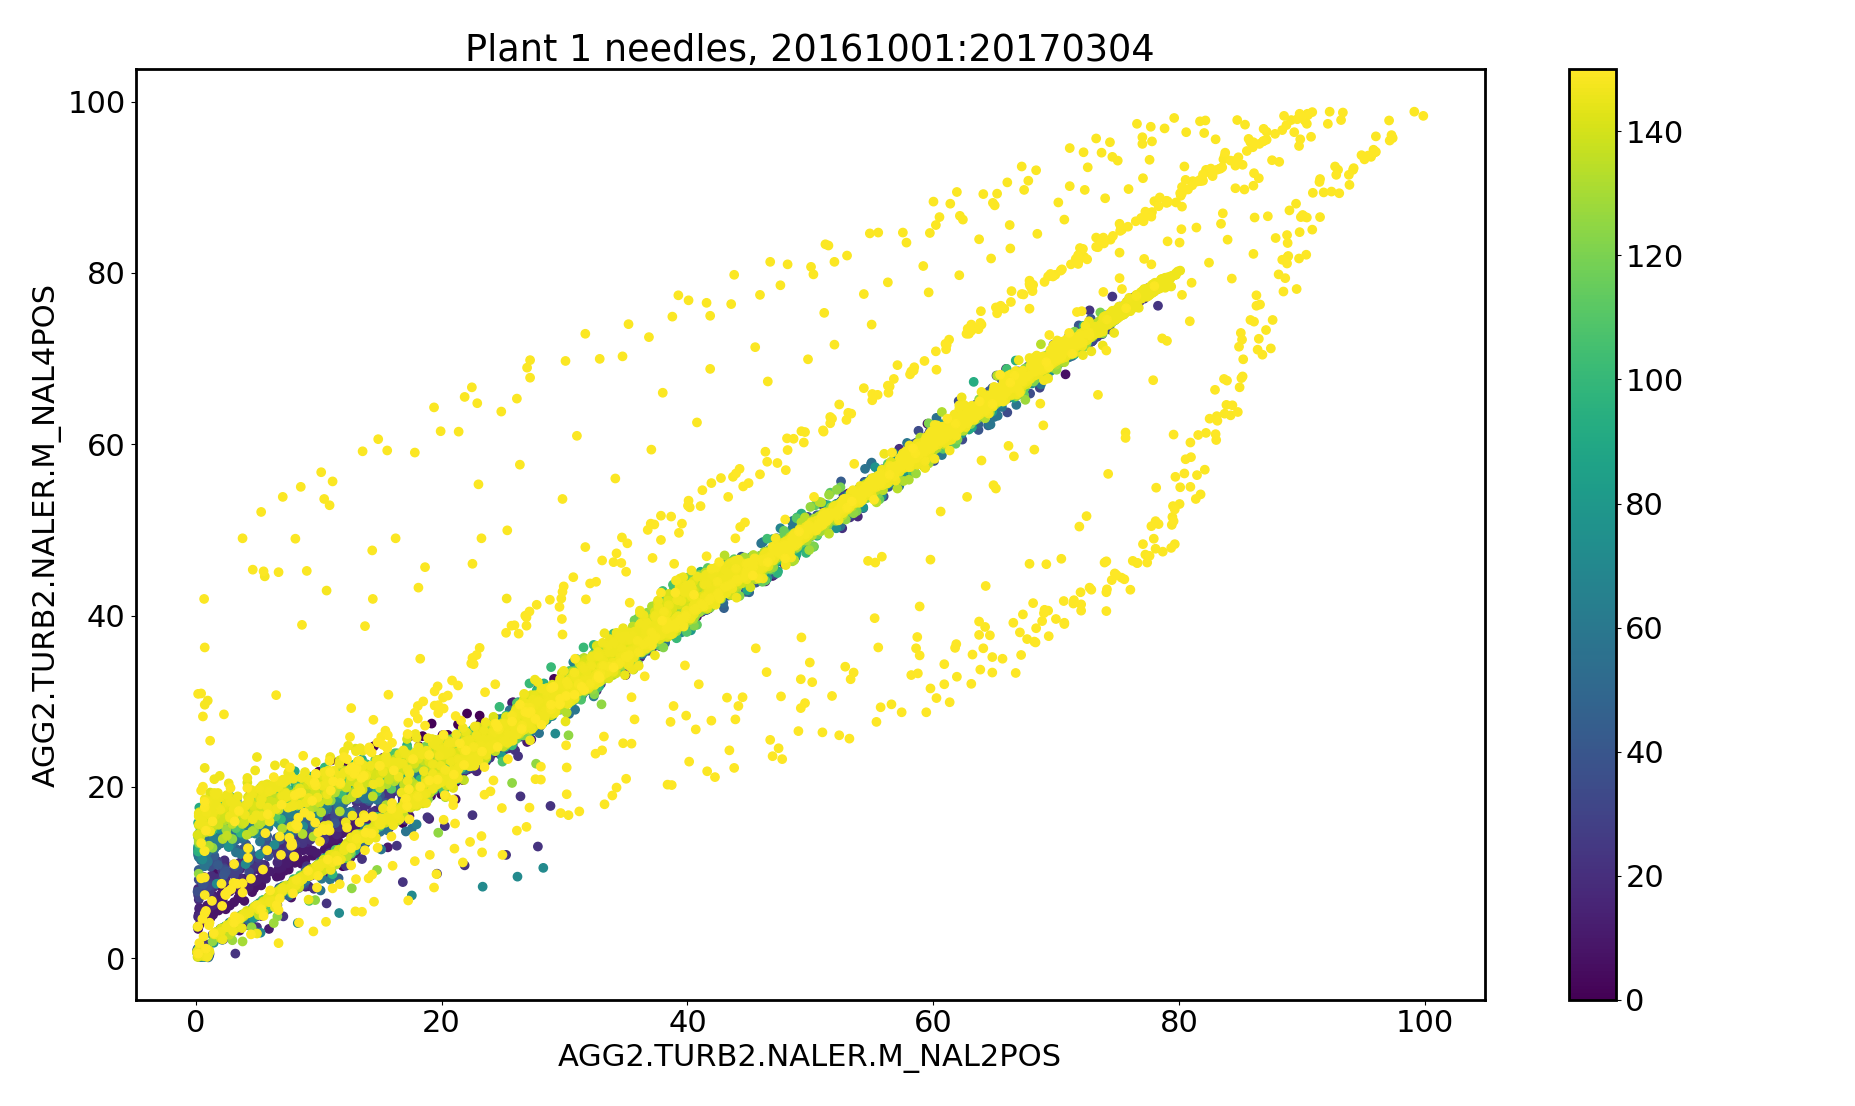
\includegraphics[width=\textwidth]{report/figures/analysis/plant1_error/needle_2_4_20161001-20170304_dots.png}
            \caption{Scatterplot of needle 2 and 4 at Plant 1 turbine 2 of the 150 days leading up to the incident. The color of a sample indicates when it is sampled. The color bar to the right shows how the color change with time. Day 0 is 150 days before the incident. The opening of needle 2 is along the x-axis, and the opening of needle 4 is along the y-axis.}
            \label{fig:plan1_scatter_20161001-20170304}
        \end{figure}
        Figure \ref{fig:plan1_scatter_20161001-20170304} shows a scatter plot of the needles [2,4] for the last 150 days up to the reported incident. The sample color changes as days go by, as seen in the color bar. It becomes clear that the most deviating samples are from the days around the incident. There are very few dark samples that deviate from the linear pattern, indicating normal system operation 150 days before the incident. Figure \ref{fig:plan1_scatter_20161001-20170304_40} shows the same plot zoomed in. Looking at the bottom left corner of the plot, one can see that needle 4 is lagging behind needle 2. It is also clear that the lag is worsening with time, as the color is shifting from dark to yellow. What happens the day of the incident is hard to explain, and the data takes on a completely new pattern. Unfortunately, it was not possible to get the full information from the energy company about what maintenance was performed to fix this problem. It is therefore assumed that the incident is a result of the system degradation seen leading up to 02.03.2017 and that this pattern can be used to detect similar system degradation before the performance becomes unacceptable.     
        \begin{figure}
            \centering
            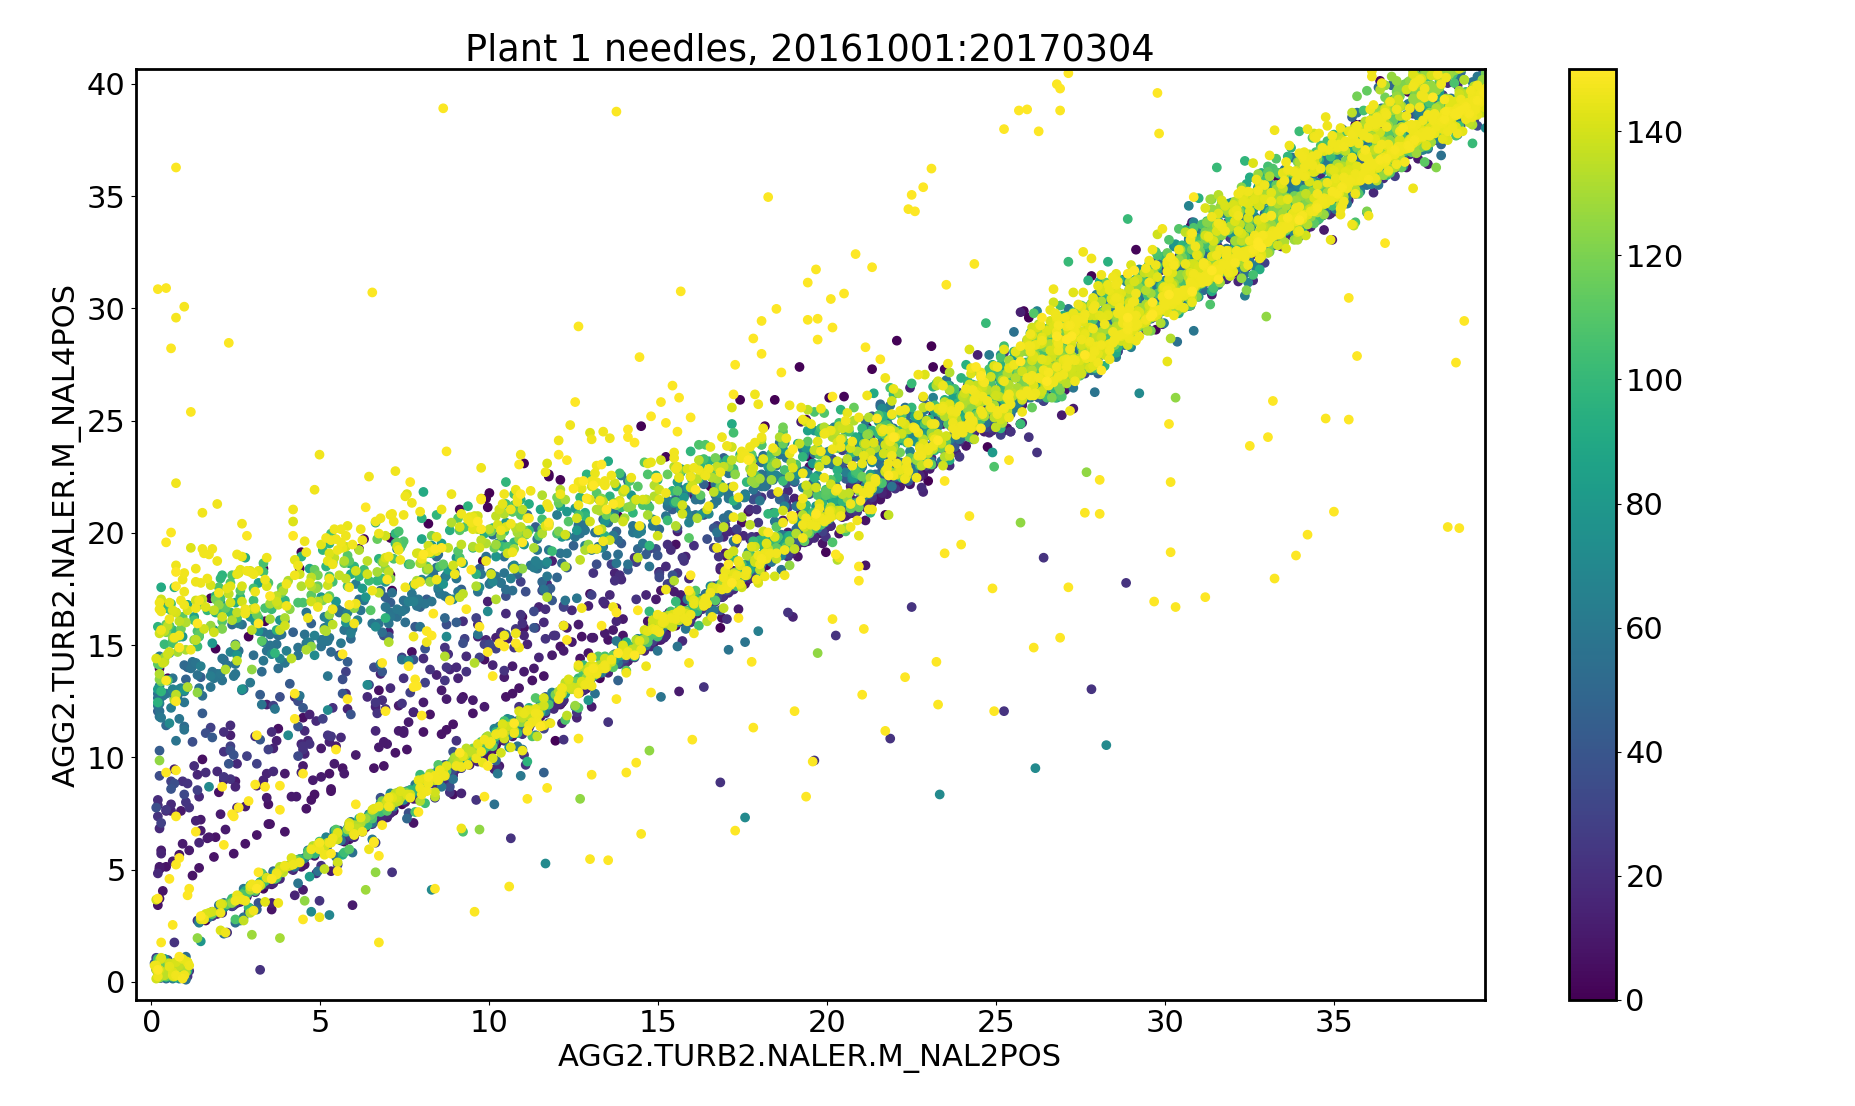
\includegraphics[width=\textwidth]{report/figures/analysis/plant1_error/needle_2_4_20161001-20170304_40_dots.png}
            \caption{Turbine 2 needle [2,4] scatterplot of the 150 days leading up to the incident zoomed in. How to interpret the figure can be seen in Figure \ref{fig:plan1_scatter_20161001-20170304}.}
            \label{fig:plan1_scatter_20161001-20170304_40}
        \end{figure}
        
        % \begin{figure}[h!]
        %     \caption*{Turbine 2 needle positions}
        %     \begin{minipage}[b]{0.5\linewidth}
        %         \centering
        %         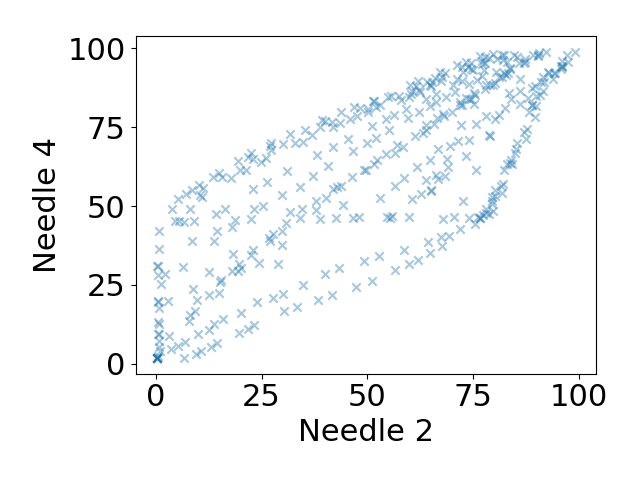
\includegraphics[width = \textwidth]{report/figures/data/turb2_n2_n4_02032017.png}
        %         \caption{02.03.2017}
        %         \label{fig:n_pos_0203}
        %     \end{minipage}
        %     \begin{minipage}[b]{0.5\linewidth}
        %         \centering
        %         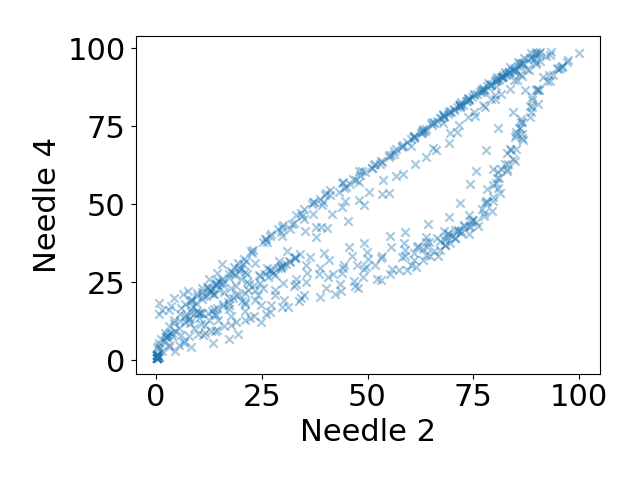
\includegraphics[width = \textwidth]{report/figures/data/turb2_n2_n4_03032017.png}
        %         \caption{03.03.2017}
        %         \label{fig:n_pos_0303}
        %     \end{minipage}
        %     \begin{minipage}[b]{0.5\linewidth}
        %         \centering
        %         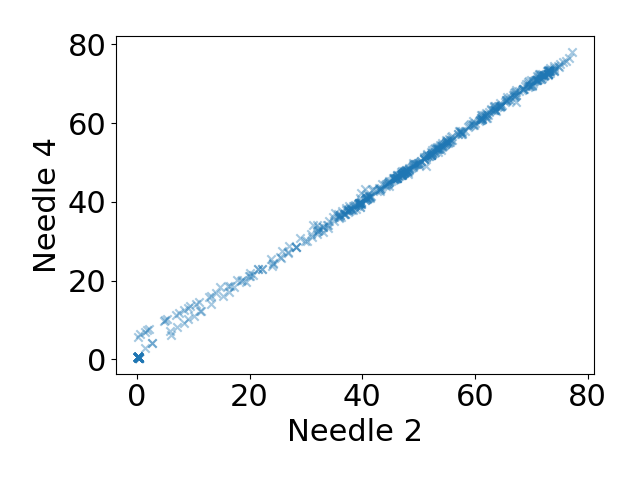
\includegraphics[width = \textwidth]{report/figures/data/turb2_n2_n4_after_04032017.png}
        %         \caption{04.03.2017 ->}
        %         \label{fig:n_pos_aft_0303}
        %     \end{minipage}
        % \end{figure}
        
        To investigate how the turbine had performed earlier in the sampling period, Figure \ref{fig:plant1_needle_error} was created. It shows the needles positions on top of each other, and the error between them. The reported incident $02.03.2017$ can be seen in the plot. The claim made earlier that the system is gradually degrading can be supported by the growing error up to the incident. Interestingly, there also seem to have been some issues with the operation in both 2014 and 2016. There is, however, no reported incidents in the plant log. 
        \begin{figure}
            \centering
            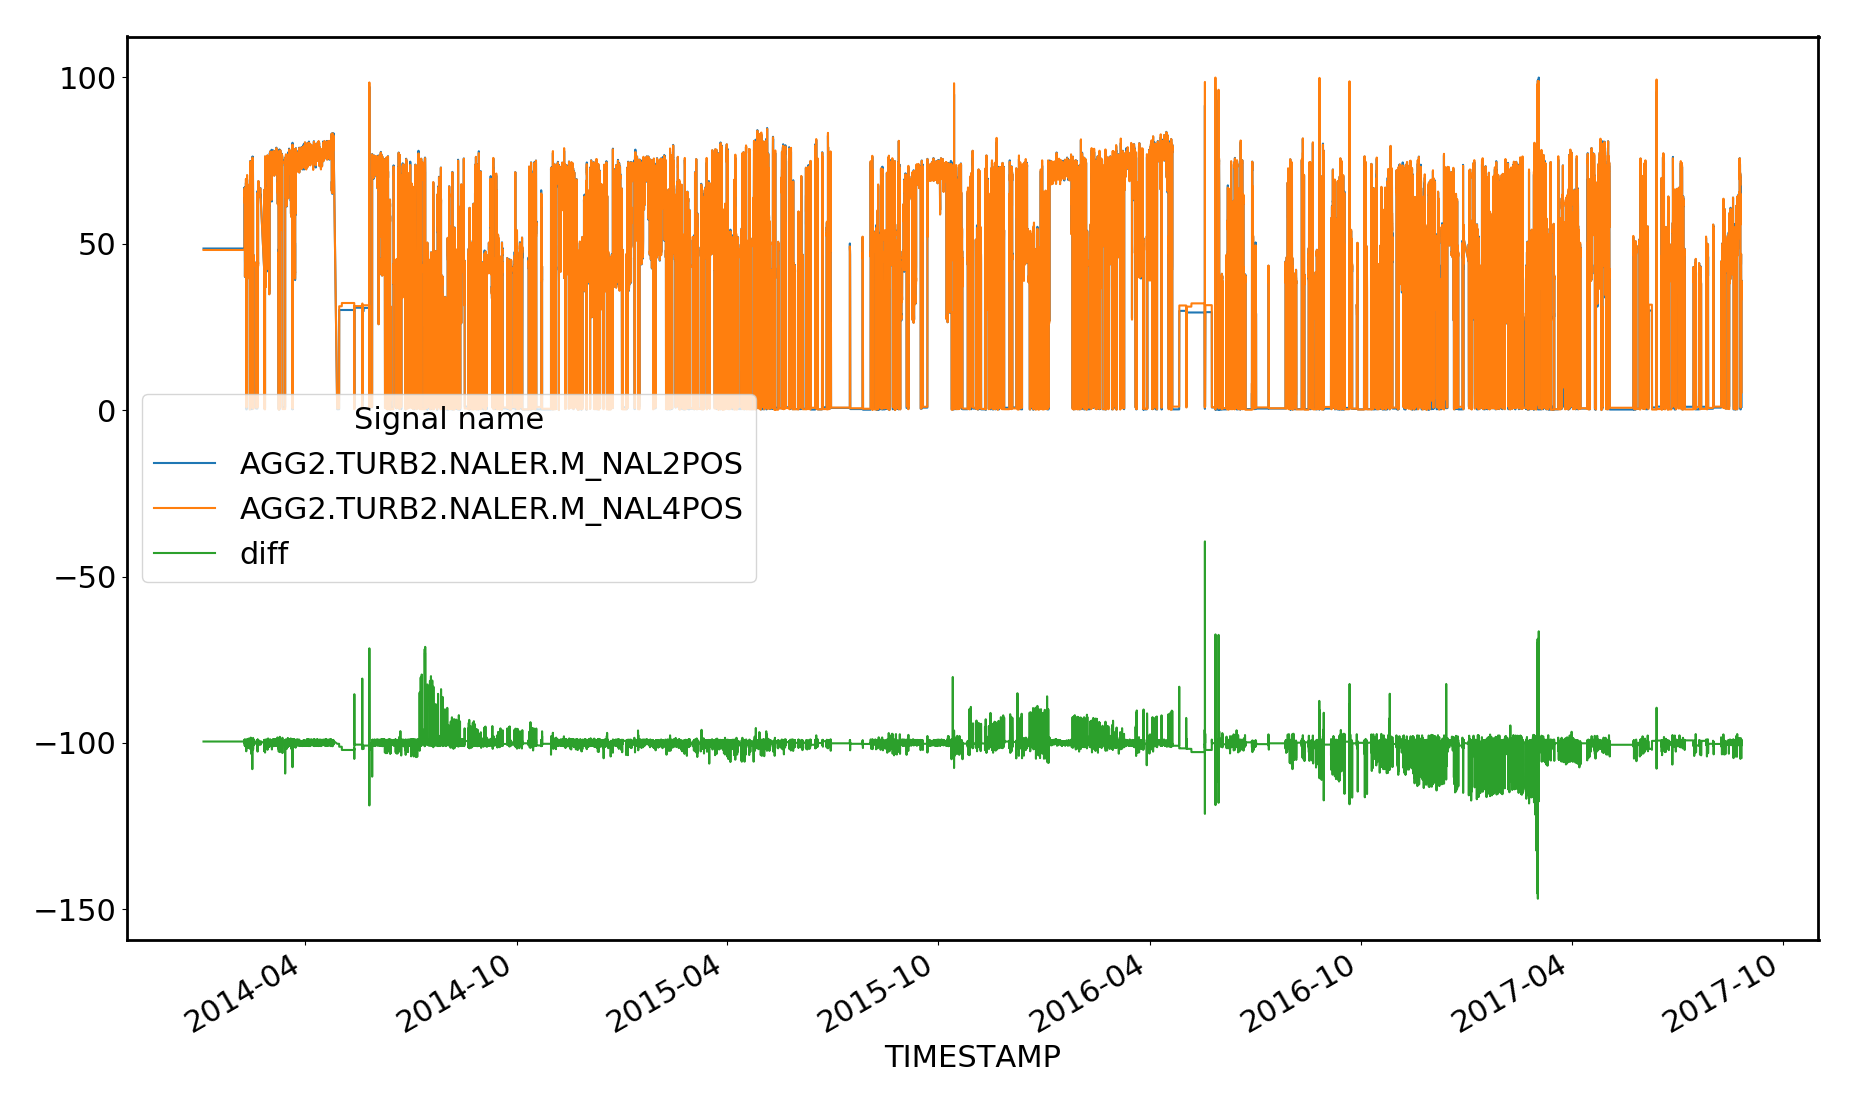
\includegraphics[width=\textwidth]{report/figures/data/turbine2_needle2_4.png}
            \caption{Needle 2 and 4 plotted on top of each other is seen in orange and blue at the top of the figure. With an offset of -100 the needle difference is seen in green. The dates are seen along the x-axis.}
            \label{fig:plant1_needle_error}
        \end{figure}
        
        
    \subsection{Other Pelton needle incidents}\label{subsec:start_failures}
        The log reported two other issues with the turbine needles at Plant $1$, that is observable in a scatter plot. This is seen in Figure \ref{fig:start_failure_turb1} and \ref{fig:start_failure_turb2}. Both are start-up failures due to problems with the needle operation.
        \begin{figure}[h!]
            % \caption*{Start up errors}
            \begin{minipage}[b]{0.49\linewidth}
                \centering
                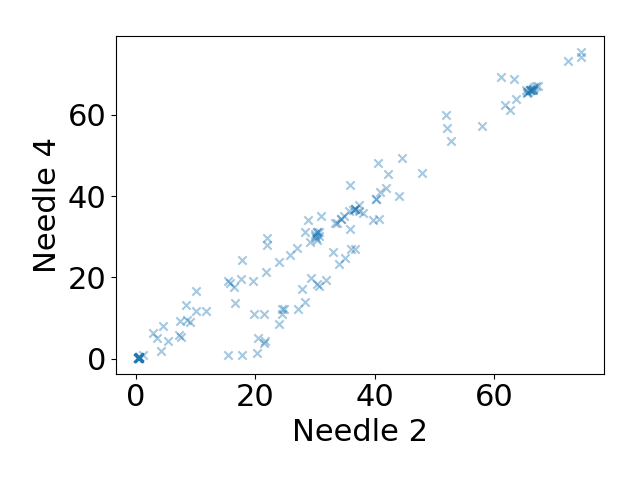
\includegraphics[width = \textwidth]{report/figures/data/turb1_n2_n4_scatter_start_failure_10122014.png}
                \caption{Turbine 1 start failure, 10.12.2014. Pairwise operated needles are scatterplotted against each other.}
                \label{fig:start_failure_turb1}
            \end{minipage}
            \hfill\vline\hfill
            \begin{minipage}[b]{0.49\linewidth}
                \centering
                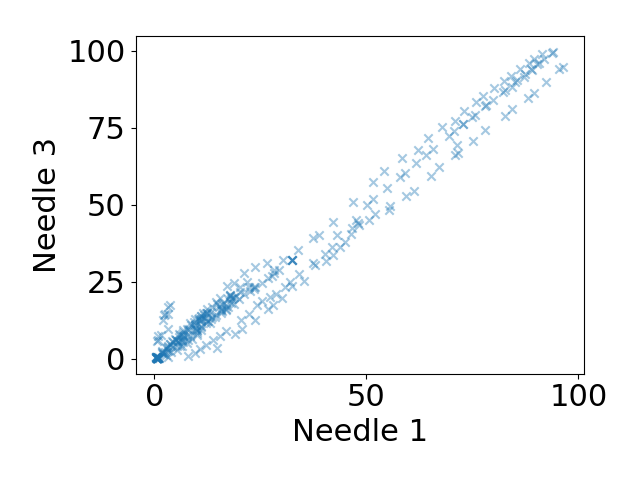
\includegraphics[width = \textwidth]{report/figures/data/turb2_n1_n3_start_failure_25082016.png}
                \caption{Turbine 2 start failure, 25.08.2016. Pairwise operated needles are scatterplotted against each other.}
                \label{fig:start_failure_turb2}
            \end{minipage}
        \end{figure}
        
        
    
    \subsection{Other plants with Pelton turbines}
        Further investigation showed that the second plant with Pelton turbines also has two turbines with pairwise operated needles. The third Pelton plant only has one turbine, and the needles are not pairwise operated. The turbine use from 1 to 5 needles depending on the produced power. Data from this plant could be used to generalize the anomaly detection methods to handle any combination of needles, but this will not be covered in this thesis. The needle operation for the second plant is seen in Figure \ref{fig:plant2_needles}. One can see that turbine $1$ has no sampling on needle $1$, but the three other pairs are sampled correctly. Plant 2 further motivates that there is something wrong with the needles for plant $1$. All needle pairs follow the linear pattern much better and have very few anomalies.
        \begin{figure}
            \begin{minipage}[b]{0.5\linewidth}
                \centering
                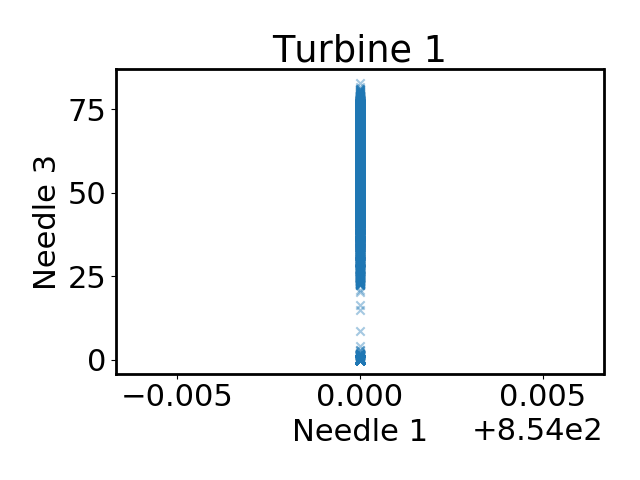
\includegraphics[width=\textwidth]{report/figures/data/p2_t1_n1_n3.png}
            \end{minipage}
            \begin{minipage}[b]{0.5\linewidth}
                \centering
                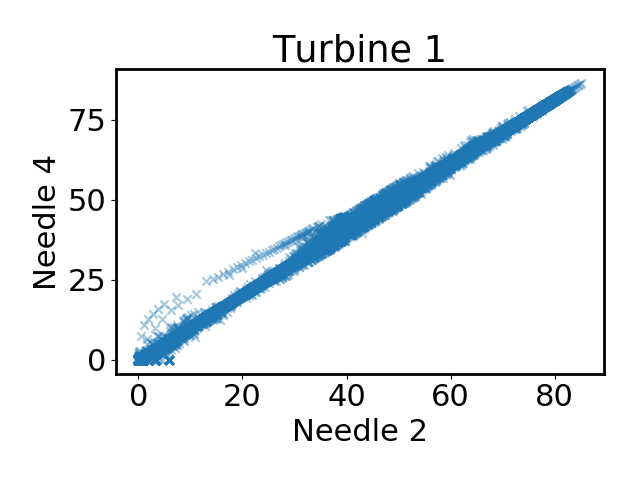
\includegraphics[width=\textwidth]{report/figures/data/p2_t1_n2_n4.png}
            \end{minipage}
            \begin{minipage}[b]{0.5\linewidth}
                \centering
                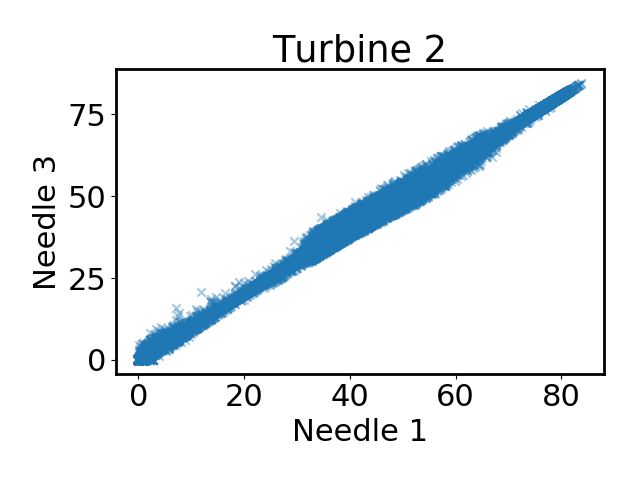
\includegraphics[width=\textwidth]{report/figures/data/p2_t2_n1_n3.png}
            \end{minipage}
            \begin{minipage}[b]{0.5\linewidth}
                \centering
                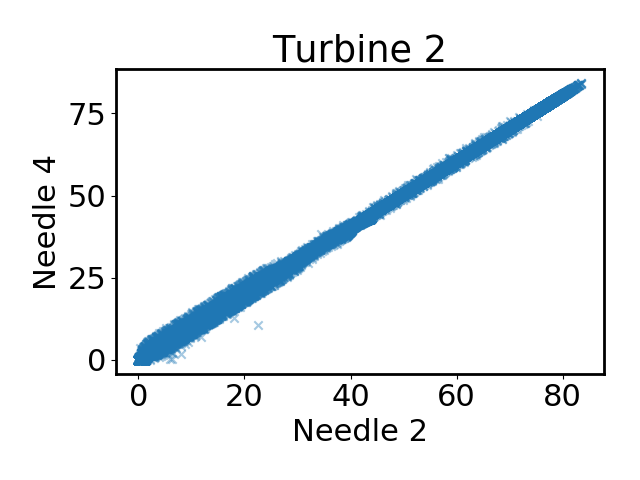
\includegraphics[width=\textwidth]{report/figures/data/p2_t2_n2_n4.png}
            \end{minipage}
            \caption{Needle openings for the pairwise operated needles for both turbines at Plant 2 are scatterplotted in four sub-figures.}
            \label{fig:plant2_needles}
        \end{figure}
        
        
        
    % \section{Other process signals}
        
    
        
    %     mention that this alone is a case one can build upon but track the error to other process-variable would be very interesting both for condition monitoring but also for identification of the fault and why it happened. 
        
        
    %     It is important to understand that an outlier in the data does not necessarily mean that something is about to break. There is a possibility that the sample is an indication of a condition change in the equipment, but it might also be due to an error in the measurement, noise or just a deviation in the ongoing process. This makes this kind of analysis even harder. An outlier might be coincident, that yields little to no information. 
        
         
         
    \subsection{Artificial needle error}\label{subsec:arti}
        Due to not having any incidents similar to the one seen at plant 1 turbine 2, an artificial error replicating the error is created. The primary motivation is to see when an error that is increasing over time is detectable. A subset of the data sampled at plant 2 is altered to replicate an error similar to the one seen for plant 1. By doing so, one knows exactly when the error starts occurring. This can then be used to evaluate how early different anomaly detection techniques detect anomalies.
    
        The turbine needles are controlled through a hydraulic system. A hydraulic system can suffer from many problems which can cause operational problems, such as pressure drops due to both external and internal leakage. External leakage is often broken hoses or pipes. Internal leakages are within the pumps and actuators. Both types of leakages reduce the system pressure and can slow down the motion of the system. Oil contamination can also be an issue if filters are not maintained at a given interval, unfiltered oil can then lead to clogged components, which can lead to pressure drops. The leading theory of the problems seen at plant 1 is that the oil flow is restricted in one direction. As needle 4 closes, the larger the differential pressure caused by the water head being restricted becomes. As the differential pressure grows, closing the needle requires more force. This means that if the hydraulic system is suffering from reduced capacity in one direction, the motion of the needle will slow down as the needle close. 
        
        Figure \ref{fig:plant2_arti_error} shows the colored scatter plot for the plant 2 data with and without the artificial error. As can be seen, it has a very similar pattern to what was seen at plant 1 in the days leading up to the reported incident. Figure \ref{fig:plant2_arti_error_40}, shows a close up on the lower openings of the needle. The deviation between the two needles increases with time, as seen in the case of plant 1. The artificial error is added to data sampled from needle pair [2,4] on turbine 2 at Plant 2. Data from 20161001 to 20170401 is used, and the artificial error is added from 20170201.     
        
        \begin{figure}
            \begin{minipage}[b]{0.5\linewidth}
                \centering
                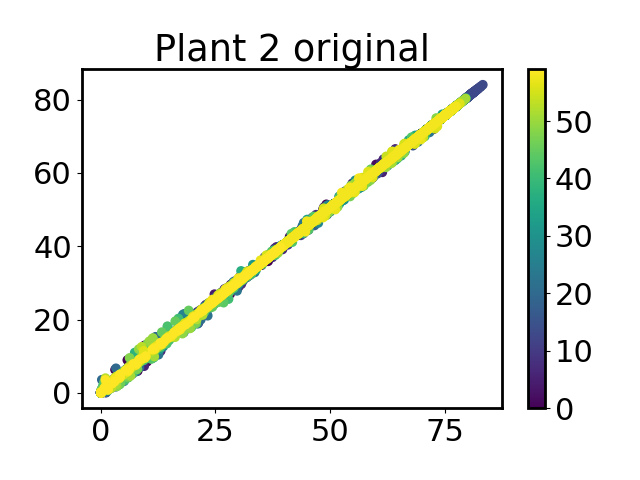
\includegraphics[width = \textwidth]{report/figures/analysis/artificial error/original_data_small.png}
                % \caption{Original data}
                % \label{fig:plant2_arti_orig}
            \end{minipage}
            \begin{minipage}[b]{0.5\linewidth}
                \centering
                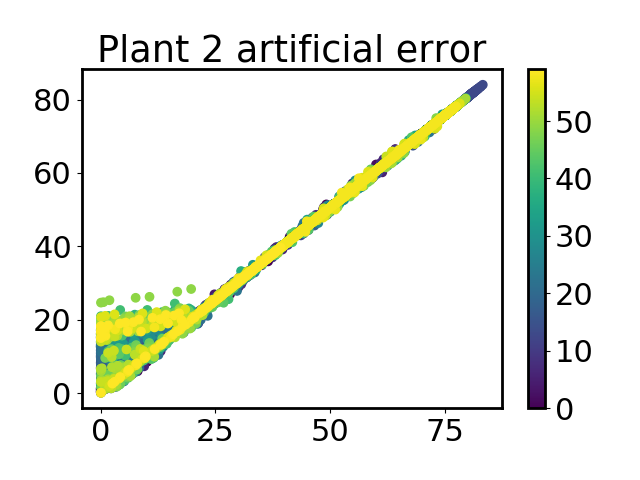
\includegraphics[width = \textwidth]{report/figures/analysis/artificial error/plant2_arti_error_small.png}
                % \caption{Added artificial error}
                % \label{fig:plant2_arti_error}
            \end{minipage}
            \caption{Colored scatter plot of the data before and after adding the artificial error. The original data is seen in to the left. How to interpret the figure can be found in Figure \ref{fig:plan1_scatter_20161001-20170304}.}
            \label{fig:plant2_arti_error}
        \end{figure}
        
        \begin{figure}
            \centering
            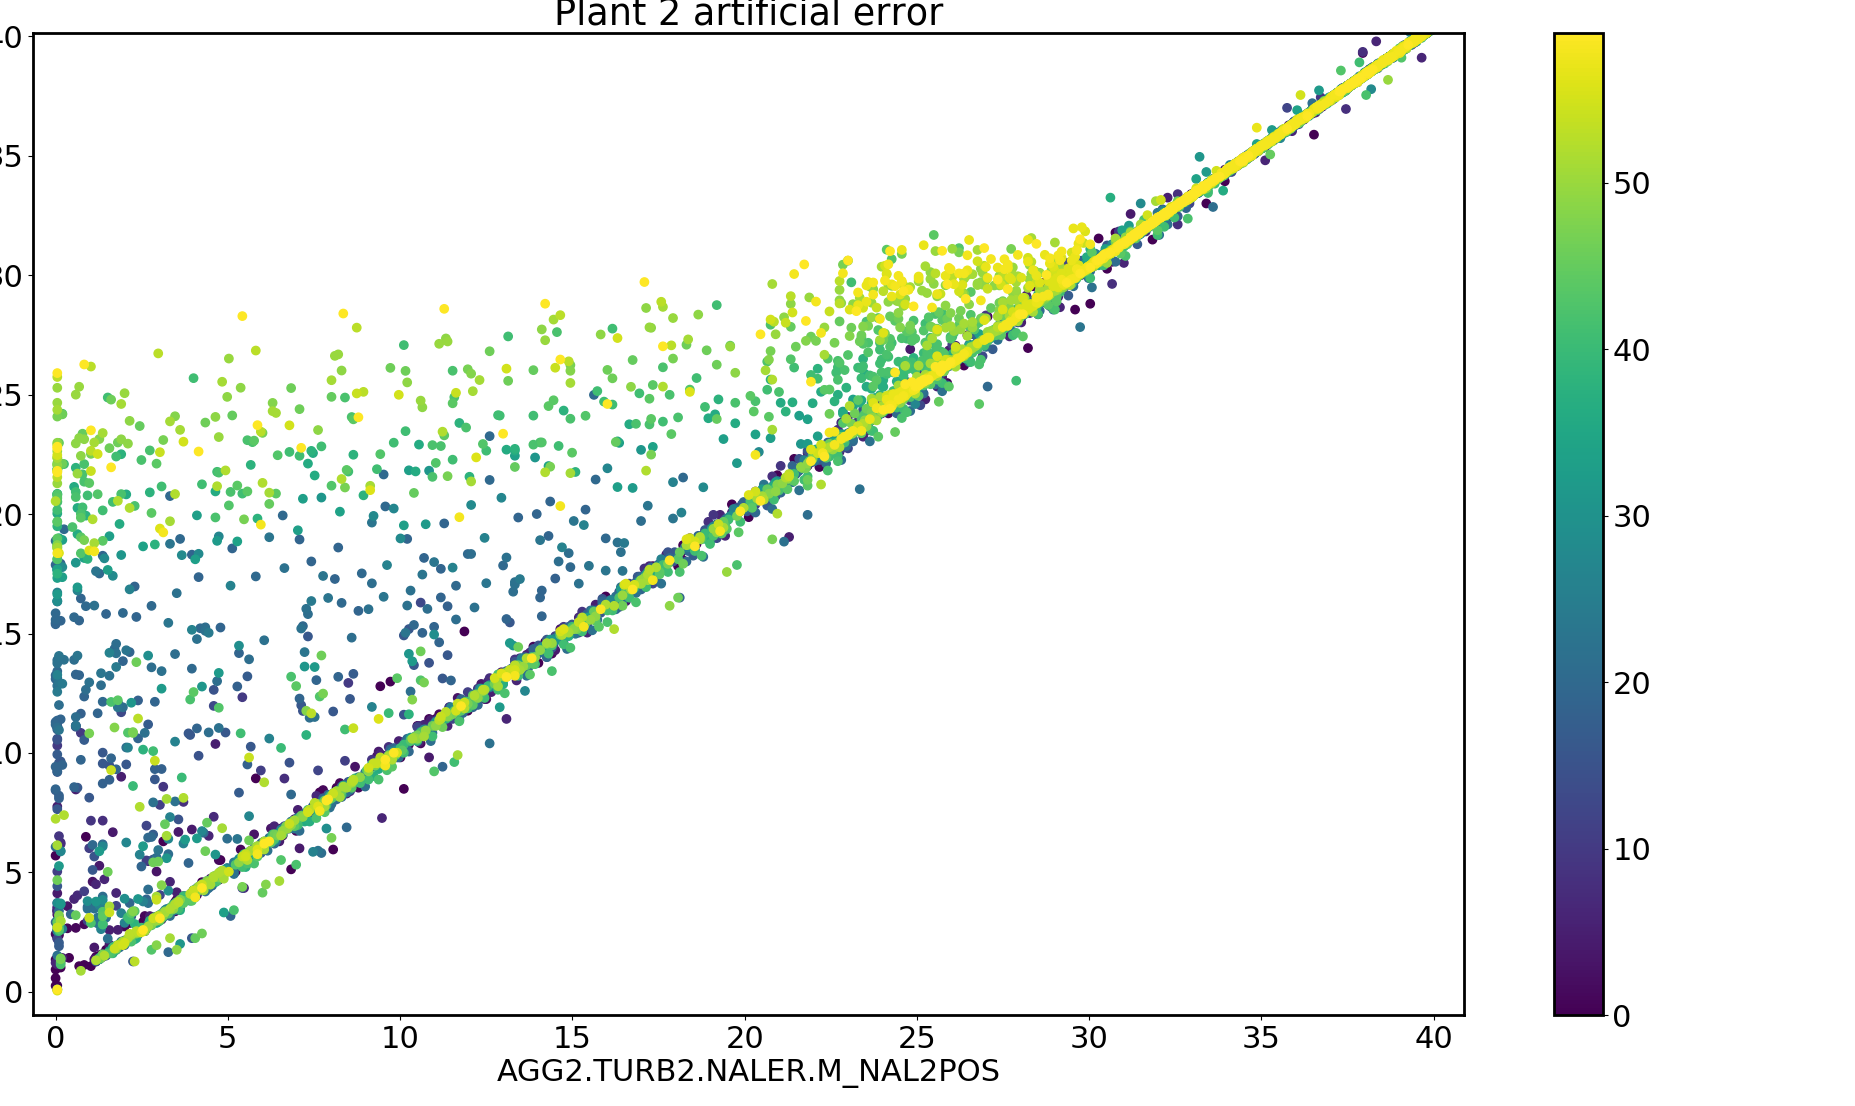
\includegraphics[width = \textwidth]{report/figures/analysis/artificial error/plant2_artificial_error_scatter_colored_40.png}
            \caption{Colored scatterplot of the artificial error for the lower openings. How to interpret the figure is found in Figure \ref{fig:plan1_scatter_20161001-20170304}.}
            \label{fig:plant2_arti_error_40}
        \end{figure}
\chapter{Analyzing the dataset and building a case}\label{cha:data}

This chapter introduces the dataset and work done to enable information extraction and analysis of the provided data. The case for the analysis is also introduced.


% In the data set, three power plants have Pelton turbines with measurement of their needle position. More information about a Pelton turbine can be found in chapter \ref{cha:data}. One of the power plants had recorded several issues with the control and behavior of the needles during operation. There were many interesting events spread out over many of the power plants, but one major benefit with the Pelton needle case was that there was one plant with several reported issues for the same component. In most of the other cases, there were only recorded one incident on one plant, making them hard to analyze and validate. The fact that there are two additional power plants with the same process signals without reported issues opened up the possibility for testing and validating the chosen techniques not only on data from the faulty plant. This also introduced the possibility to validate how well and how easy the different techniques could adapt to new plants.    




% Based on the arguments above, the Pelton needle case was chosen as the focus of the thesis. The following points were then defined as a basis for the analysis. 


\section{Dataset}\label{sec:dataset}
    Hymatek controls provided a dataset from a Norwegian energy company, containing process information from $27$ hydroelectric power plants logged from $2013$ to mid $2017$. The data is not pre-processed in any way, and come just as it is logged at the company. A big part of the thesis has been spent on exploring the data, finding out what is logged and what can be used. The data is split into five folders, one for each year. In each folder, several different files are stored. Table \ref{tab:data_files} shows the different file types that are found in the dataset. The file names indicated the frequency, sampling type and sampling duration of the data. The files are not separated by plants, only by date. Hence, a file containing data sampled every second for any given start and stop date contains data from all plants for that given period. In addition to the data files, a meta-data file is provided where plant name and process signal for each tag can be found.
    
    \begin{table}[]
        \centering
        \begin{tabular}{c c c c c}
        
        \toprule
             \textbf{Interval}   & \textbf{Average}   & \textbf{Max}   & \textbf{Min}   & \textbf{Actual}    \\ \midrule
             Daily      & x         & x     & x     & -         \\ 
             Hourly     & x         & x     & x     & -         \\ 
             Minutely   & x         & x     & x     & -         \\ 
             Secondly   & -         & -     & -     & x         \\ \bottomrule
        \end{tabular}
        \caption{Table showing the available data for the different sampling frequencies}
        \label{tab:data_files}
    \end{table}
    
    The total size of all files exceeded $90$Gb. This means that one can't merely load all data into the computer memory, and work with it from there. The information needs to be extracted one plant at a time, for each of the different sampling rates and stored in a way that enabled fast and efficient loading.

    
    \subsection{Old and new data format}\label{subsec:data_format}
        Regardless of sampling-rate and data type, the files are all in the same format. As seen in Table \ref{tab:orig_data}, each line holds a tag, a time of sampling and process value. 
        \begin{table}[h]
            \centering
            \begin{tabular}{c c c}
                \toprule
                 \textbf{Tag}        & \textbf{Timestamp}         & \textbf{Value}  \\ \midrule
                 192390514  & 20170101000000000 & 0.897244155 \\
                 192391514  & 20170101000000000 & -0.549806237 \\ \bottomrule
            \end{tabular}
            \caption{Example of the structure of the original datasets}
            \label{tab:orig_data}
        \end{table}
        Once a file is loaded the tag is replaced by the process-signal name found in the meta-data file. To enable interpretation and analysis of the data, it is decided that new datasets needs to be created on the format shown in Table \ref{tab:plant_format}.
        \begin{table}[h]
            \centering
            \begin{tabular}{c c c c c }
                \toprule
                \textbf{Time stamp} & \textbf{P. variable 1}     & \textbf{P. variable 2}    & \textbf{..}    & \textbf{P. variable n}    \\ \midrule
                time 1        & NaN         & $2$           & ..    & NaN         \\ 
                time 2        & $3.00$      & NaN           & ..    & $0.00214$\\ 
                :            & :            & :             & ..    & : \\ 
                time n        & $1.00$      & NaN           & ..    & $0.814$\\ \bottomrule
            \end{tabular}
            \caption{Example showing how the data looks for each plant after reconstruction is complete}
            \label{tab:plant_format}
        \end{table}

        
    \subsection{Overview of the datasets}
        Once the data is reconstructed as specified in subsection \ref{subsec:data_format} one can look into what information it holds. The number of available process signals varies a lot, from above $250$ to below $20$, as can be seen in Figure \ref{fig:process_signal_overview}. This was used as a first stage filtering to reduce the number of plants to examine. The plants with fewer than $30$ process-signals are dropped from the analysis, reducing the number of plants in the dataset to $15$.    
        
        \begin{figure}[h]
            \centering
            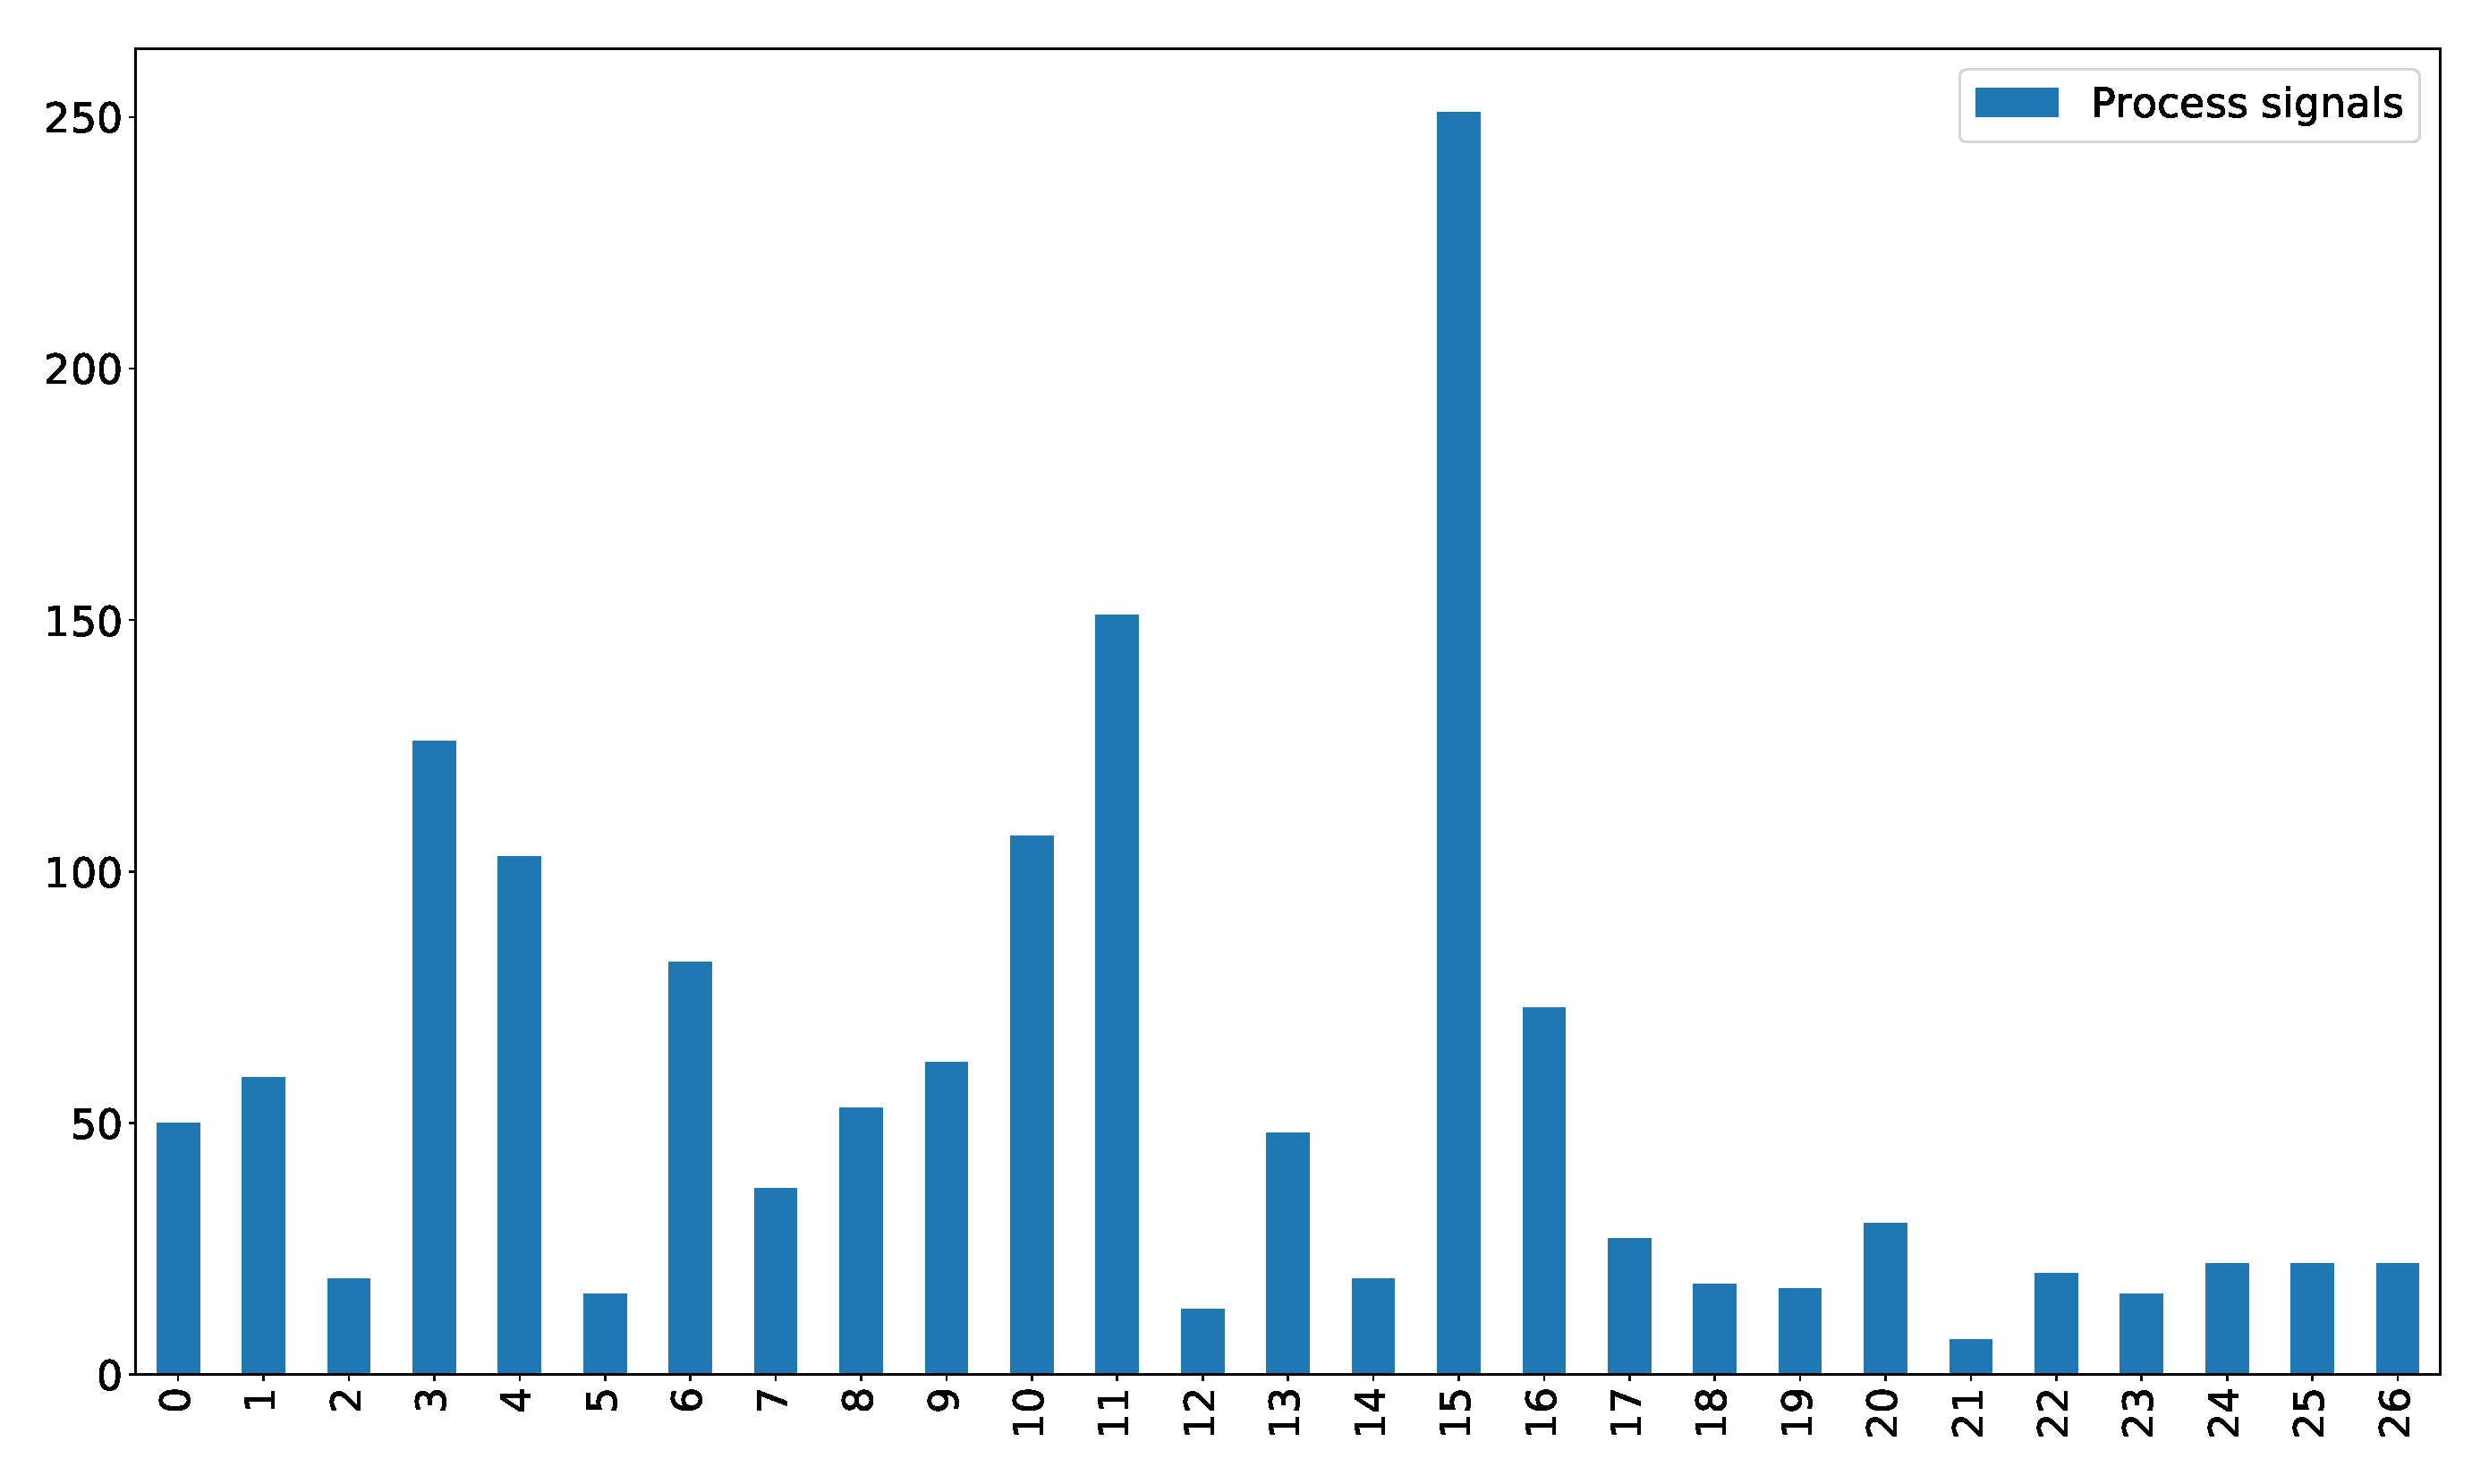
\includegraphics[width=\textwidth]{report/figures/data/plant_process_signals_overview.pdf}
            \caption{Overview of the number of process-signals or features for each of the 27 plants in the dataset.}
            \label{fig:process_signal_overview}
        \end{figure}
        
        After discarding the plants with few signals, the type of process-signals available is looked into. The more data sampled from different parts of a plant, the better. Having data from several parts and components of a plant can enable finding a link between unknown components and sensors. Figure \ref{fig:signal_type_overview} shows the different types of signals found in the datasets for the different plants. As can be seen, the temperature is one of the most common signals for all plants. There are also many signals of type "Def Type Måling", which is a common name that covers all signals not defined with a unique tag. Pressure, level, vibration, and so on are signals covered by this tag. Since all of the remaining plants has process-variables of different types, none are removed. 
        
        \begin{figure}
            \centering
            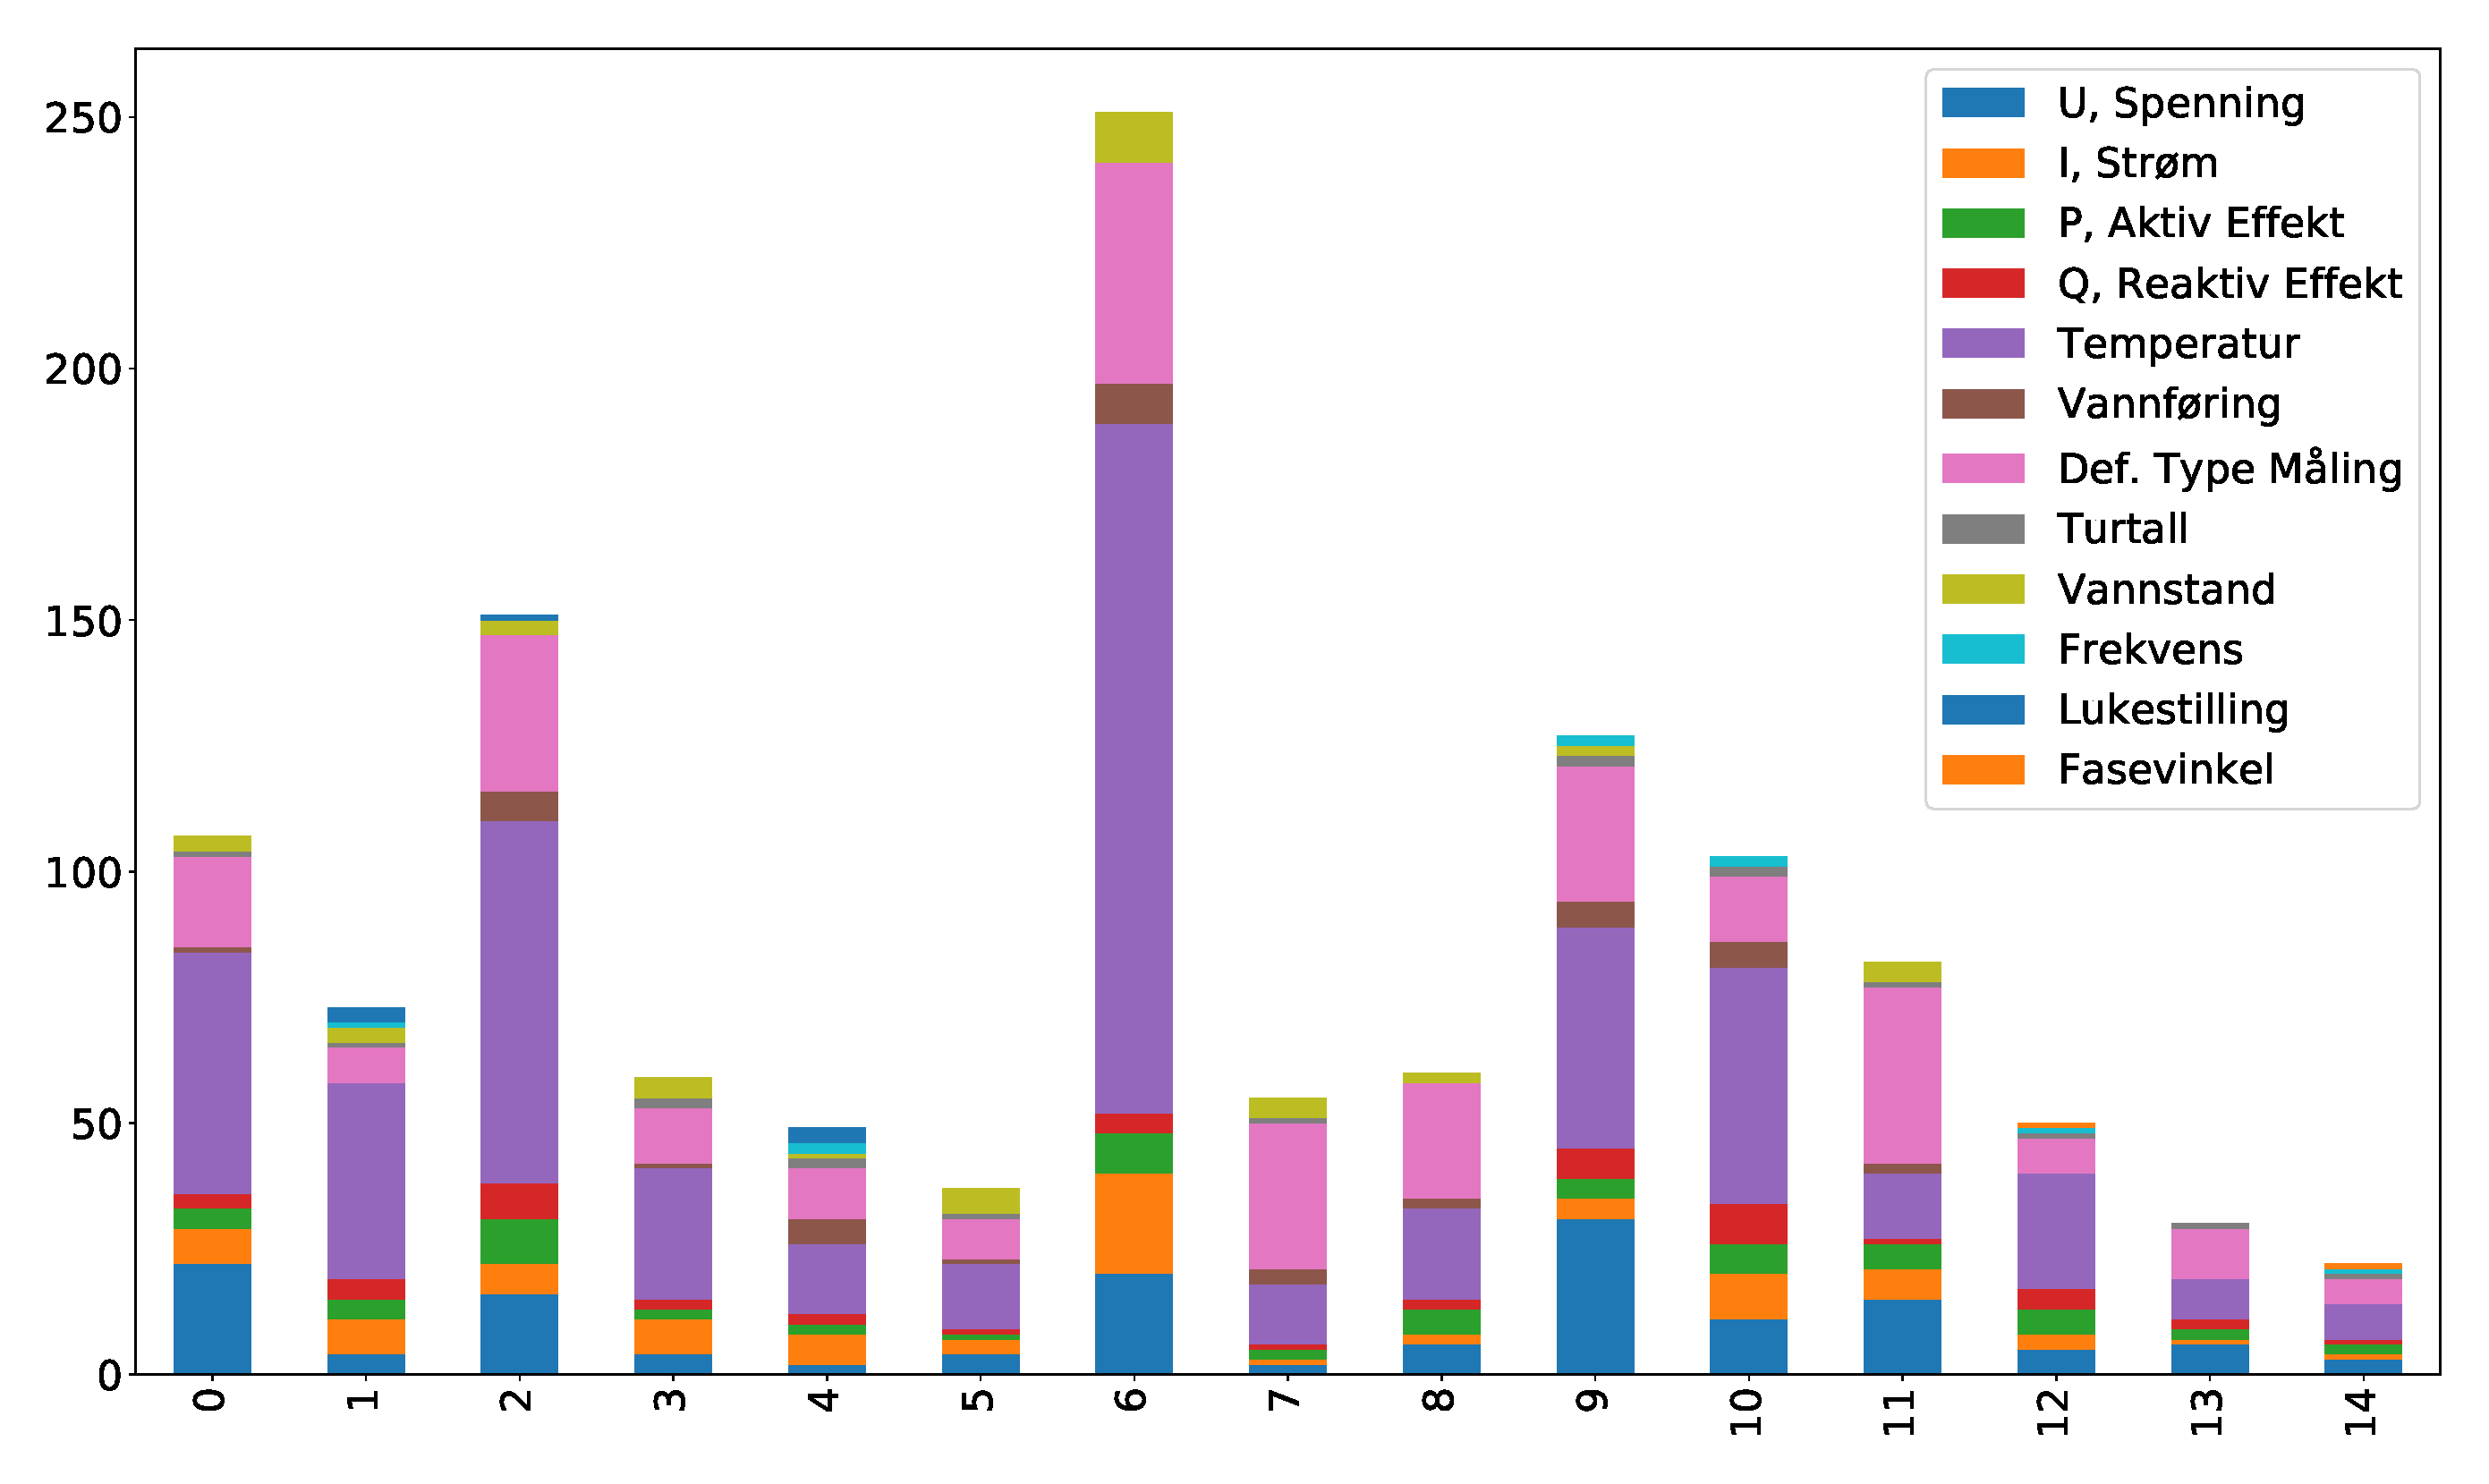
\includegraphics[width=\textwidth]{report/figures/data/plant_signal_types_overview.pdf}
            \caption{Figure showing the different process signals or features found at each of the 27 plants in the dataset.}
            \label{fig:signal_type_overview}
        \end{figure}
        
        % It is only necessary to keep the datasets with the highest sampling rate. The highest sampling rate will provide the most detail about a plant, and lower sampling rates can always be extracted from higher rates.
        
        % was decided to only use the datasets sampled every second. Using these datasets gave a snapshot of the plant state at a given time. Pandas have a lot of built-in functionality that enables easy re-sampling so that the average, max and min datasets could easily be recreated from this dataset if wanted.
        
        An issue arose when looking in detail at the datasets. Preferably, all process-signals should be sampled periodically and at the same time. This is however not the case, only at hourly resolution are the data matrices complete. At higher sampling rates there are a lot of missing data. At the highest sampling frequency (every second), there are many time-stamps where none of the process signals are sampled, and those that are sampled, often only samples one process-signal. This means that one either has to work with only hourly sample rate, work with incomplete datasets or reduce the number of process signals to investigate. Either the equipment used for sampling is not working as it should, or the varying sampling rate must be on purpose. It could be that a similar sampling scheme to the one seen in \cite{Selak2014} is used. This is however not possible to confirm from the data alone, and the energy company did not provide this information. This sheds light on the fact that having lots of data is not always a sign of quality. The data sampled in $2013$ is poorer than the later years, and hence it is dropped from any further analysis. 
    % \subsection{Instrumentation}\label{subsec:instrumentation}
    %     what is there of instrumentation? refer to the data I have gotten         
        
    \subsection{The historical log of the plants }
        Once an overview of the data was in place, the energy company was contacted, requesting an incident log from the remaining plants. Incident logs for the entire sampling period, for all of the $27$ power plants, were received. The level of details in the logged incidents is very varying from plant to plant. Some plants have reported over 200 incidents, while others barely exceeded 20. Many of the incidents are also minor incidents like a broken light bulb or nonfunctioning tools. Finding interesting incidents was time-consuming. Several interesting incidents were found, but very few were reported to occur more than once. Having few incidents makes it hard to separate valuable information from noise. Only having a limited number of faults can easily lead to overfitting. There is always a risk that randomness can cause the correlations and variable dependencies found. This needs to be taken into consideration when working such cases.  
        
        In the log for one of the power plants, it was found an error with the needles for a Pelton turbine. The error reported that as the opening of needle four of turbine two decreased below $46\%$, it started to lag behind needle two. The plant has two turbines that both have four needles. A search through the $14$ remaining power plants showed that there are two additional plants with Pelton turbines. These plants have however not reported any problems with the Pelton needles. This could then be a possible reference for normal operation. Also, it opens the possibility for testing how adaptable the anomaly detection methods are. 
        
        % \todo{remove this or add more analysis}When looking into the historical log of the plant, it was found that several more incidents with the Pelton needles were reported for the two turbines
        
\section{Pelton needles case}\label{sec:pelton_needles}
    The Pelton needle case was chosen for further analysis for several reasons. Firstly it is a critical part of the Pelton turbine, if the needles are not operating as they should it will affect the power produced by the turbine. The needle openings are a big part of a complex control system, that controls that the turbine holds constant speed. Finding a method that can give early warnings about incidents like the one above, means maintenance can be planned, and components overhauled before the system condition becomes too severe. Secondly, having data from different plants makes it possible to analyze how well the methods and techniques used to adapt to new data. This is an important factor, if one can develop a method that is transferable with little to no adaptation need between plants, the time for commissioning will be significantly reduced. In addition, this case fits well as an extension of \cite{Aasnes2017}, where the condition of the guide vanes for a Francis turbine was analyzed. Finally, quality and available process variables vary a lot from plant to plant. One of the most significant issues was that the majority of the process signals were not sampled at a constant frequency. The Pelton needles were found to be sampled in a manner that allowed the use of data from two separate plants.
             

    \subsection{Pelton needle incident 02.03.2017}
        As the incident reported that one needle was lagging behind another, it could indicate pairwise operated needles. This can also be justified from a practical perspective if the needles are placed opposite of each other they will give the turbine an even momentum as long as they lead the same amount of water onto the turbine. To confirm this, scatter-plots were created where each needle is plotted against the other. To enable this the needle process signals are pairwise extracted from the rest of the dataset, and all time-stamps where both needles are not sampled are removed. Figure \ref{fig:plant1_needles} shows the scatter-plot of the pairwise operated needles for both turbines at plant 1. As can be seen in all four plots, the majority of the data follows a linear dependency between the needles. However, several data-points deviate from this, especially for needle pair $[2,4]$ on turbine $2$, which had the reported incident. The plot in the bottom right corner shows what appears to be operational problems. It is only needle [1,3] on turbine 1 seen in the upper left plot, which follows the linear pattern.
        \begin{figure}
            \begin{minipage}[b]{0.5\linewidth}
                \centering
                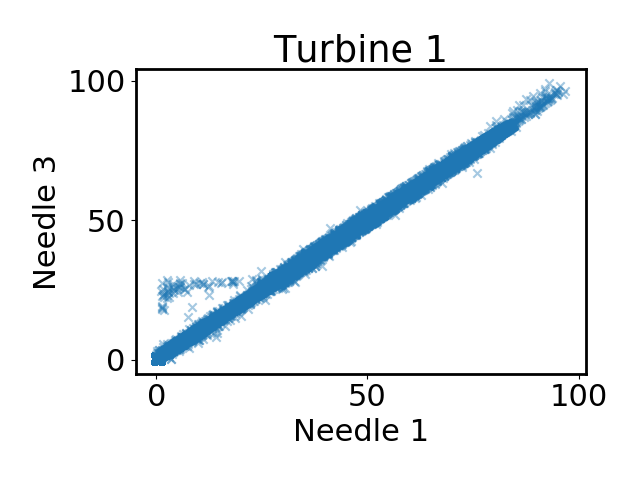
\includegraphics[width=\textwidth]{report/figures/data/t1_n1_n3.png}
            \end{minipage}
            \begin{minipage}[b]{0.5\linewidth}
                \centering
                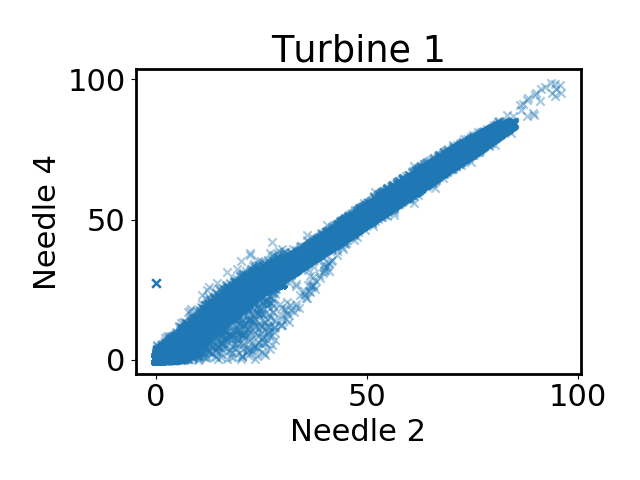
\includegraphics[width=\textwidth]{report/figures/data/t1_n2_n4.png}
            \end{minipage}
            \begin{minipage}[b]{0.5\linewidth}
                \centering
                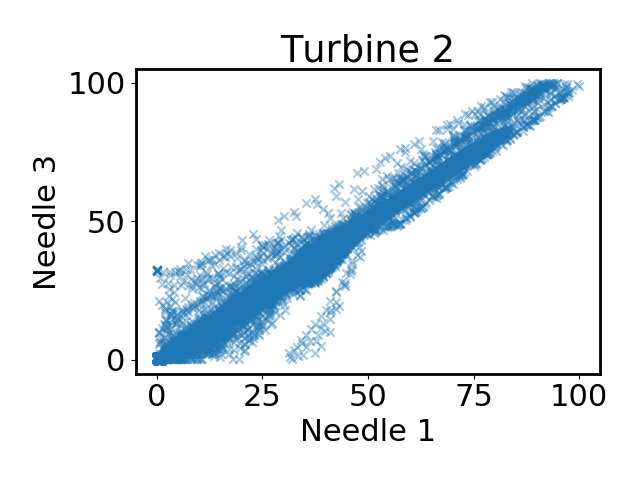
\includegraphics[width=\textwidth]{report/figures/data/t2_n1_n3.png}
            \end{minipage}
            \begin{minipage}[b]{0.5\linewidth}
                \centering
                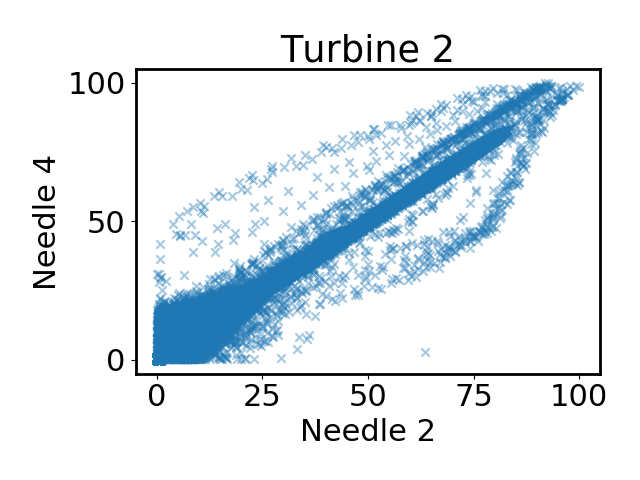
\includegraphics[width=\textwidth]{report/figures/data/t2_n2_n4.png}
            \end{minipage}
            \caption{Needle openings for the pairwise operated needles for both turbines at Plant 1 are scatterplotted in four sub-figures.}
            \label{fig:plant1_needles}
        \end{figure}
        
        % \begin{figure}[h]
        %     \centering
        %     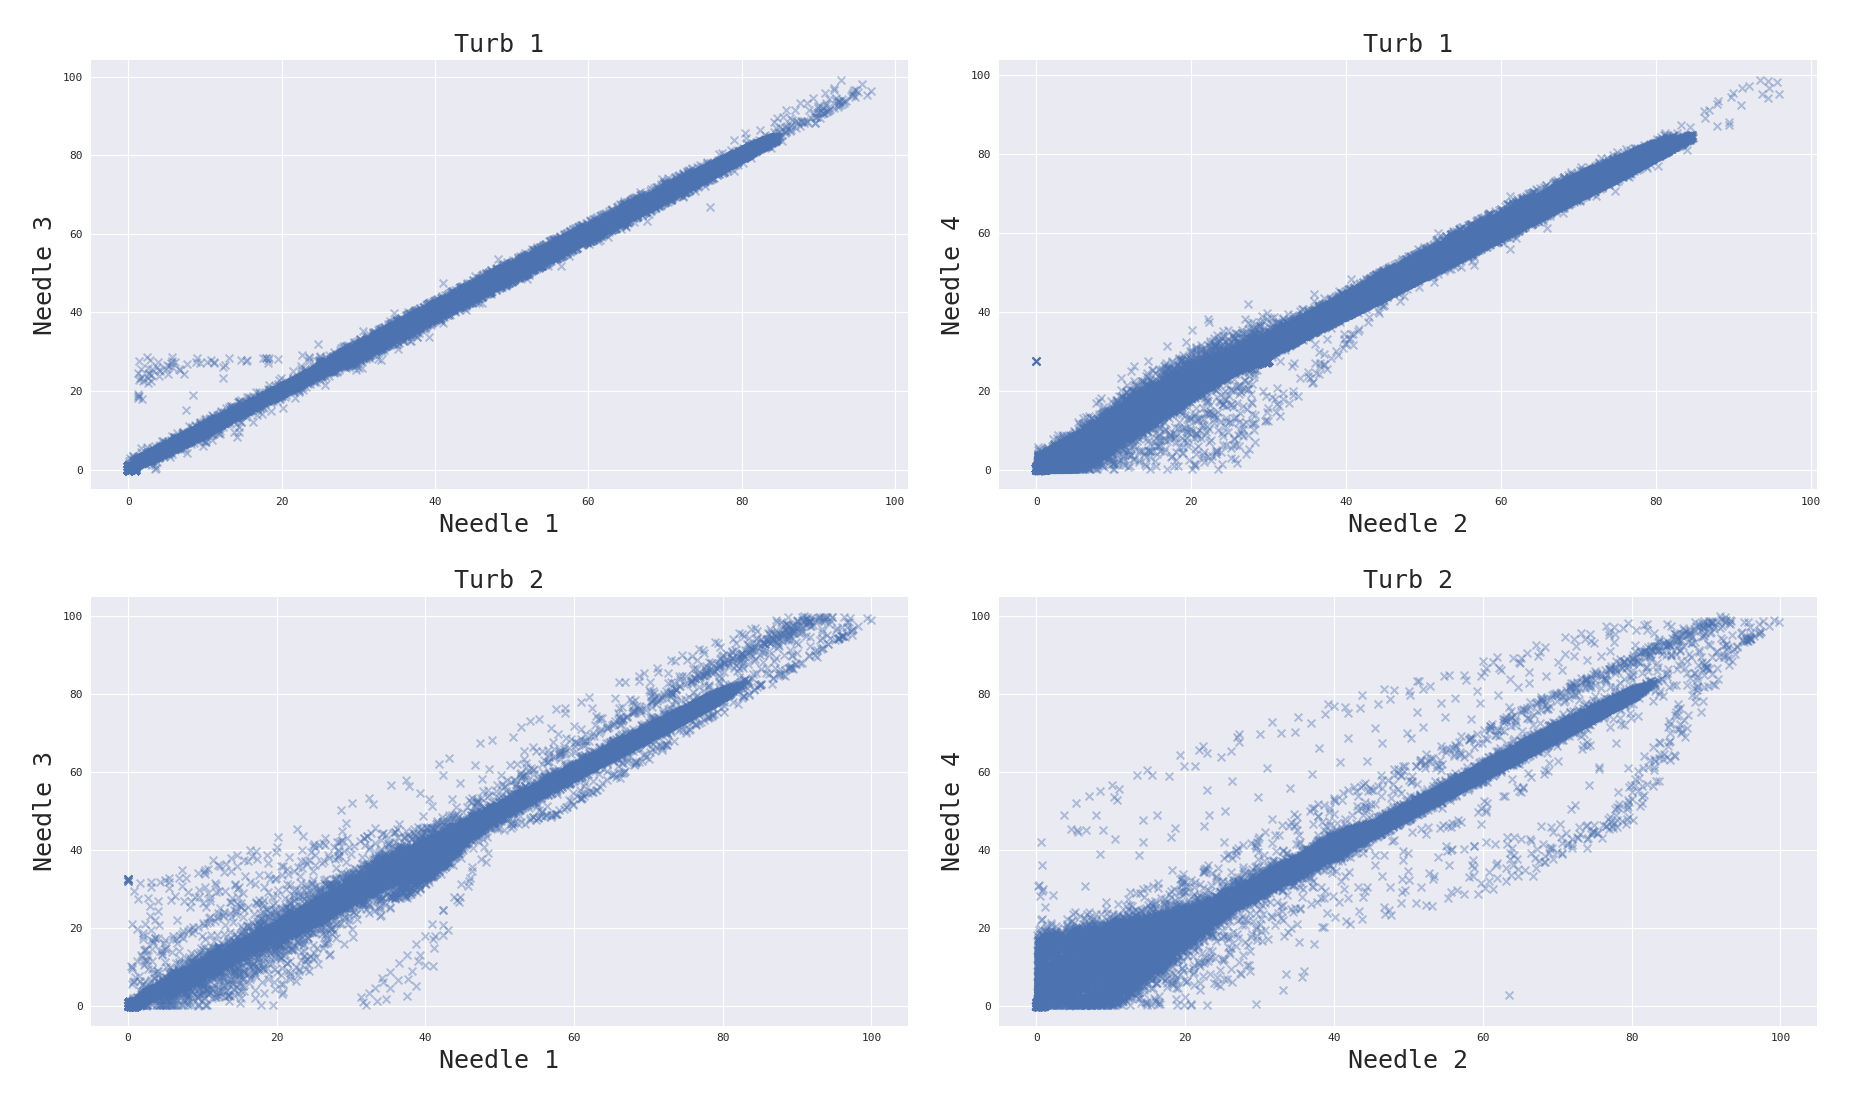
\includegraphics[width=\textwidth]{report/figures/data/plant1_needles.png}
        %     \caption{Pairwise operated needles for the two turbines at Plant 1 are scatterplotted in four subfigures. }
        %     \label{fig:plant1_needles}
        % \end{figure}
        % Figure \ref{fig:n_pos_0203} to \ref{fig:n_pos_aft_0303} shows the needle positions for two dates surrounding the reported incident, and all data after. Figure \ref{fig:n_pos_aft_0303} show that the problem was fixed when reported in early March. Figure \ref{fig:n_pos_0203} and \ref{fig:n_pos_0303} shows the two days with worst performance, and one can see that many of the worst data-points from the lower right plot in figure \ref{fig:plant1_needles}, looks to be the same as the ones shown in figure \ref{fig:n_pos_0203} and \ref{fig:n_pos_0303}.
        \begin{figure}
            \centering
            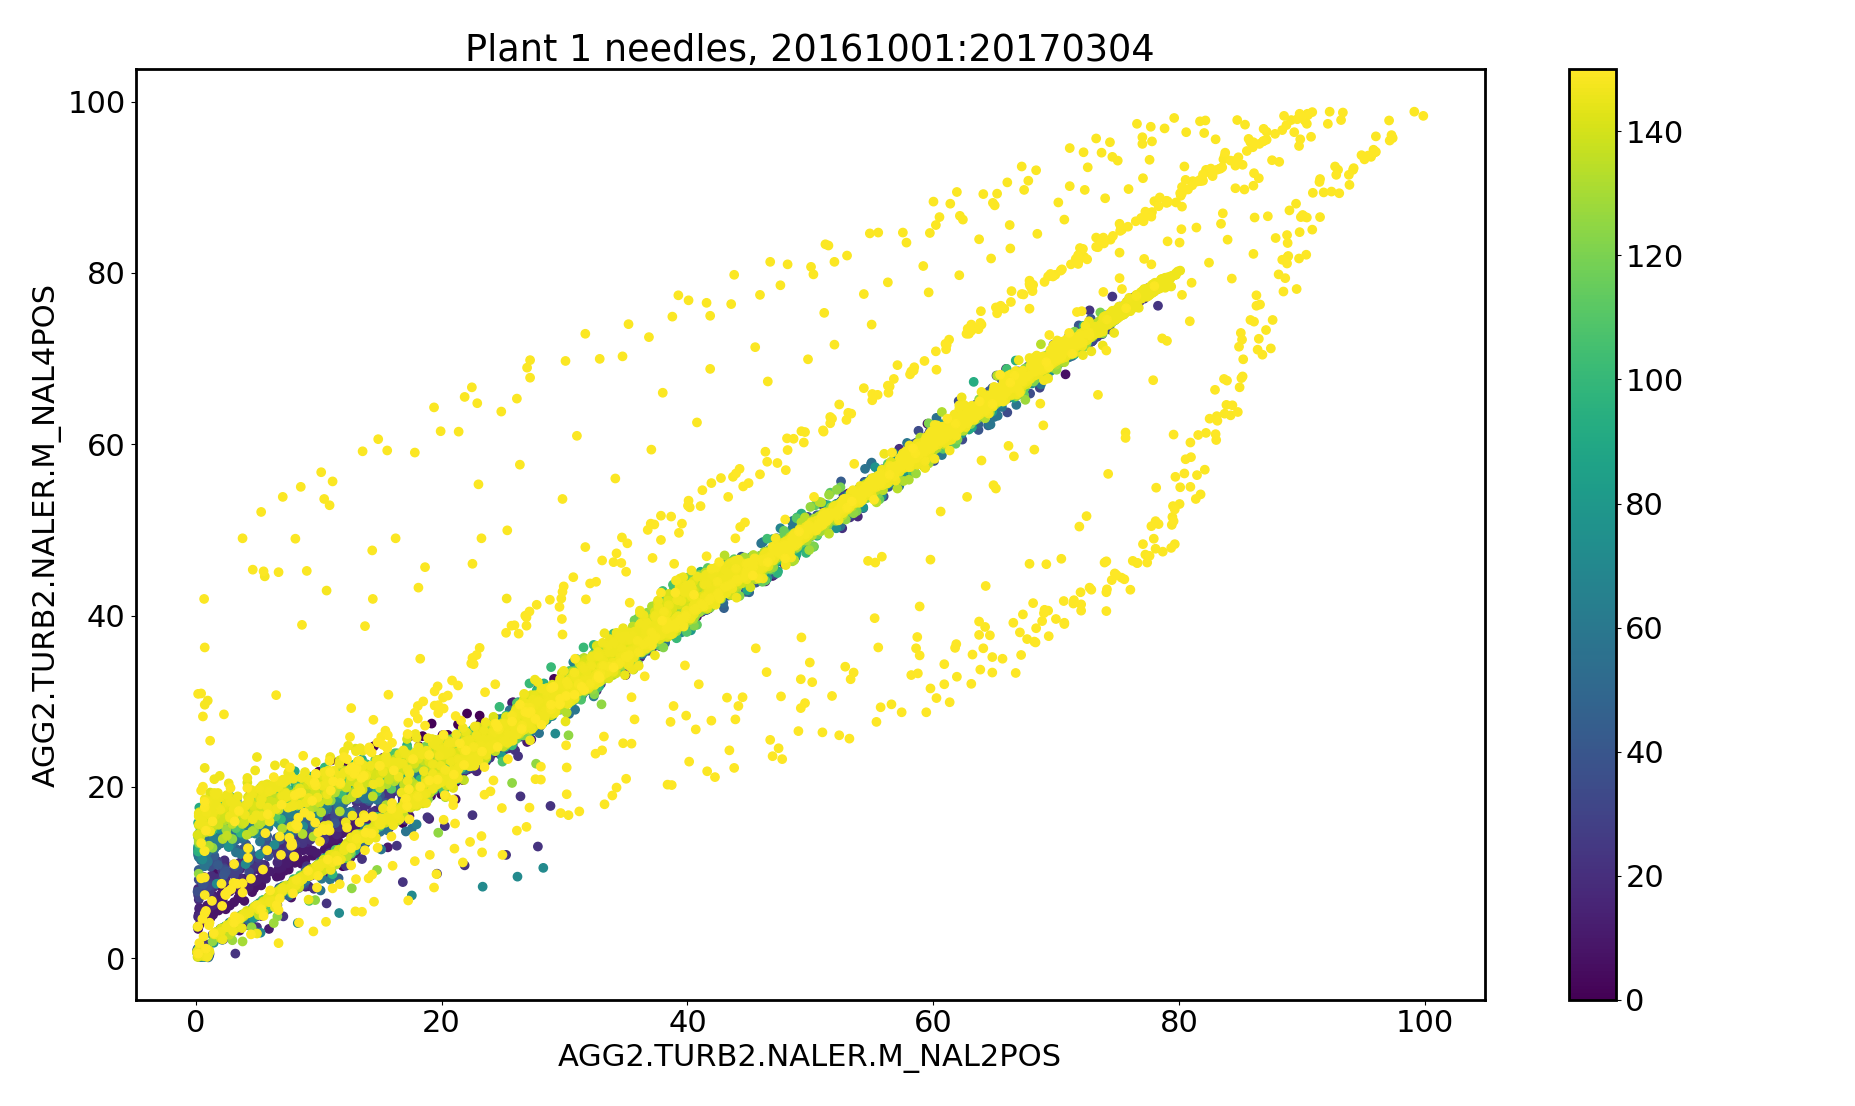
\includegraphics[width=\textwidth]{report/figures/analysis/plant1_error/needle_2_4_20161001-20170304_dots.png}
            \caption{Scatterplot of needle 2 and 4 at Plant 1 turbine 2 of the 150 days leading up to the incident. The color of a sample indicates when it is sampled. The color bar to the right shows how the color change with time. Day 0 is 150 days before the incident. The opening of needle 2 is along the x-axis, and the opening of needle 4 is along the y-axis.}
            \label{fig:plan1_scatter_20161001-20170304}
        \end{figure}
        Figure \ref{fig:plan1_scatter_20161001-20170304} shows a scatter plot of the needles [2,4] for the last 150 days up to the reported incident. The sample color changes as days go by, as seen in the color bar. It becomes clear that the most deviating samples are from the days around the incident. There are very few dark samples that deviate from the linear pattern, indicating normal system operation 150 days before the incident. Figure \ref{fig:plan1_scatter_20161001-20170304_40} shows the same plot zoomed in. Looking at the bottom left corner of the plot, one can see that needle 4 is lagging behind needle 2. It is also clear that the lag is worsening with time, as the color is shifting from dark to yellow. What happens the day of the incident is hard to explain, and the data takes on a completely new pattern. Unfortunately, it was not possible to get the full information from the energy company about what maintenance was performed to fix this problem. It is therefore assumed that the incident is a result of the system degradation seen leading up to 02.03.2017 and that this pattern can be used to detect similar system degradation before the performance becomes unacceptable.     
        \begin{figure}
            \centering
            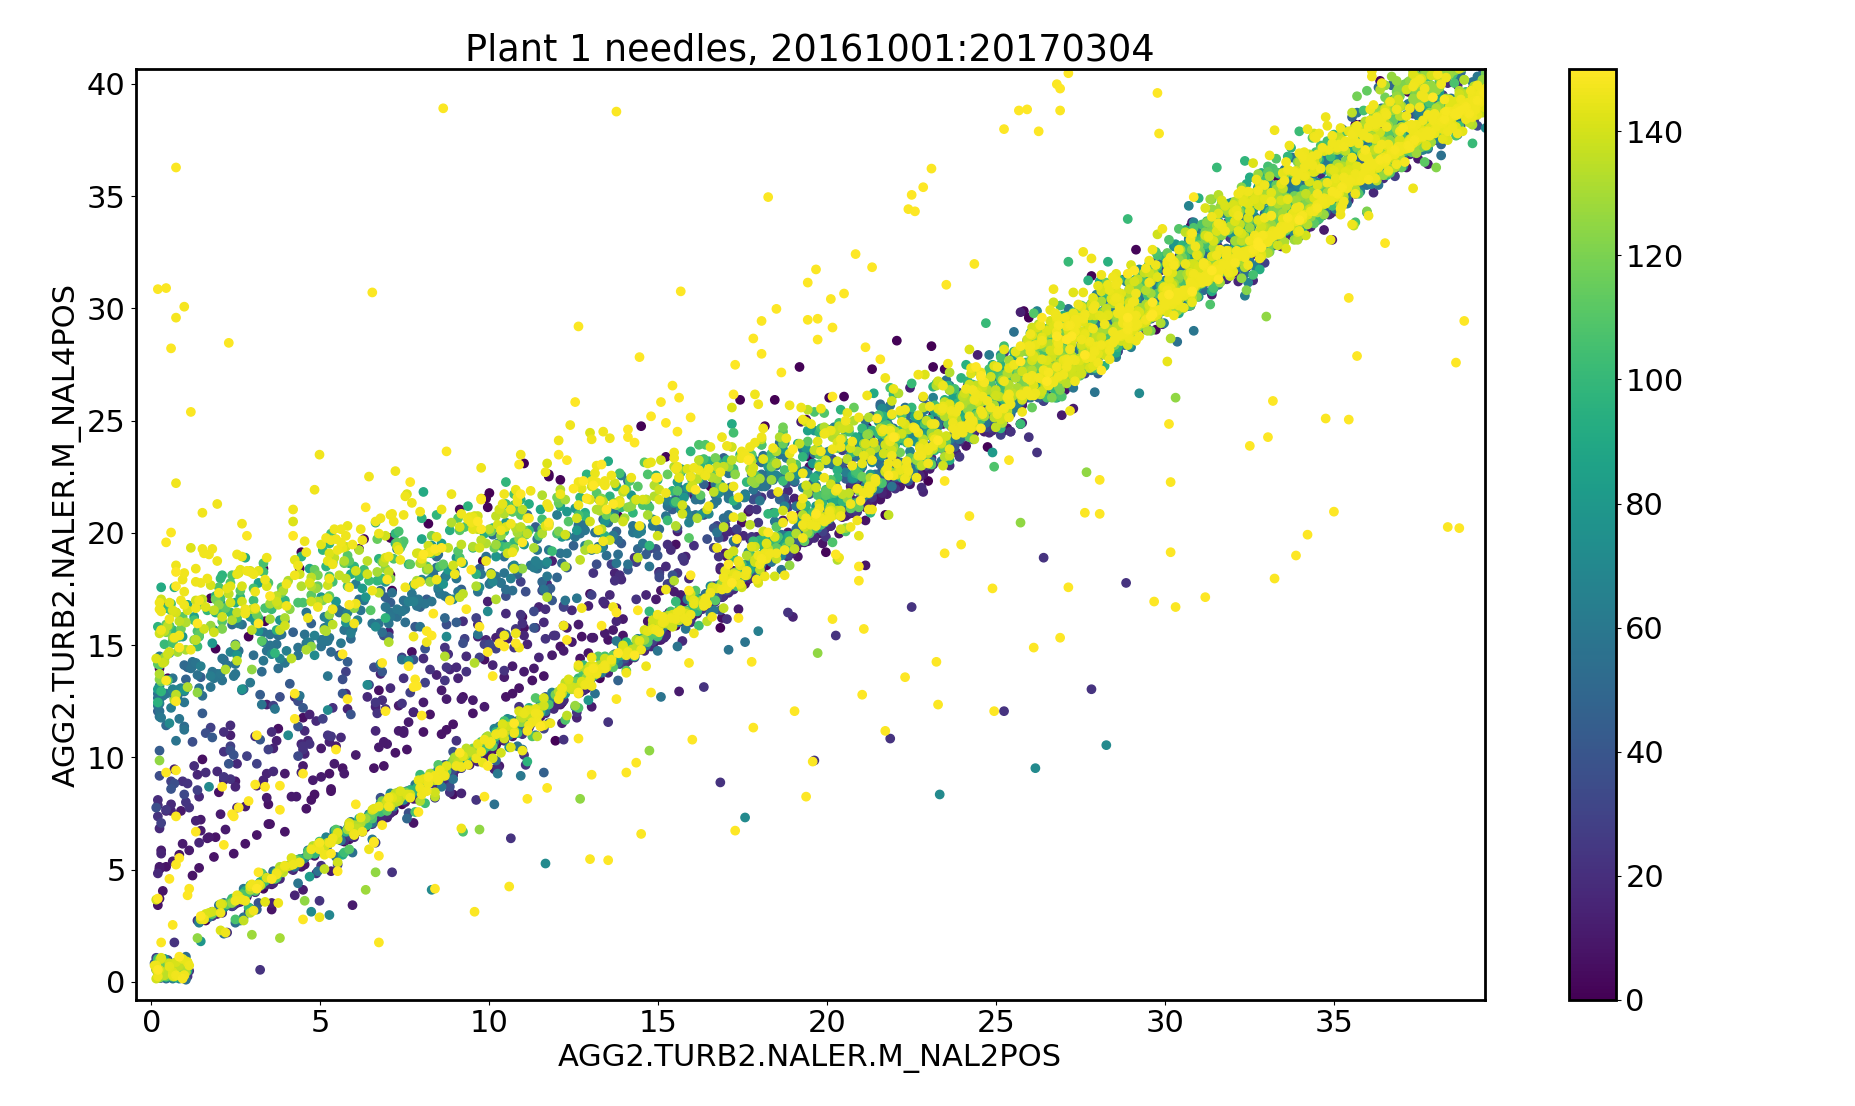
\includegraphics[width=\textwidth]{report/figures/analysis/plant1_error/needle_2_4_20161001-20170304_40_dots.png}
            \caption{Turbine 2 needle [2,4] scatterplot of the 150 days leading up to the incident zoomed in. How to interpret the figure can be seen in Figure \ref{fig:plan1_scatter_20161001-20170304}.}
            \label{fig:plan1_scatter_20161001-20170304_40}
        \end{figure}
        
        % \begin{figure}[h!]
        %     \caption*{Turbine 2 needle positions}
        %     \begin{minipage}[b]{0.5\linewidth}
        %         \centering
        %         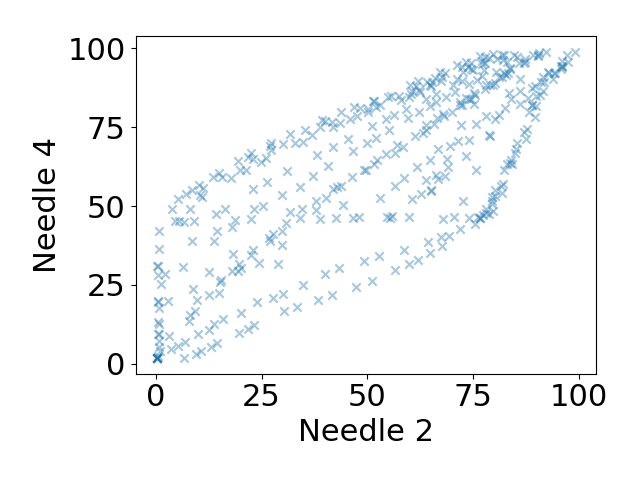
\includegraphics[width = \textwidth]{report/figures/data/turb2_n2_n4_02032017.png}
        %         \caption{02.03.2017}
        %         \label{fig:n_pos_0203}
        %     \end{minipage}
        %     \begin{minipage}[b]{0.5\linewidth}
        %         \centering
        %         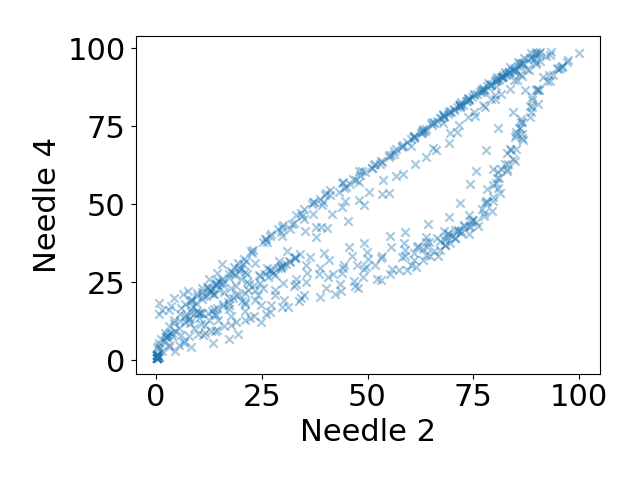
\includegraphics[width = \textwidth]{report/figures/data/turb2_n2_n4_03032017.png}
        %         \caption{03.03.2017}
        %         \label{fig:n_pos_0303}
        %     \end{minipage}
        %     \begin{minipage}[b]{0.5\linewidth}
        %         \centering
        %         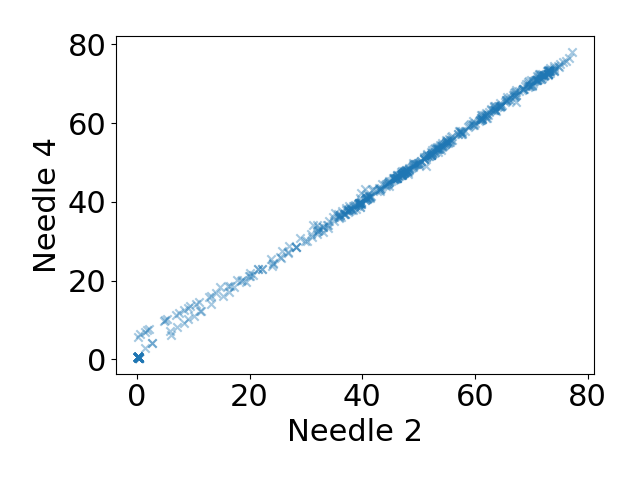
\includegraphics[width = \textwidth]{report/figures/data/turb2_n2_n4_after_04032017.png}
        %         \caption{04.03.2017 ->}
        %         \label{fig:n_pos_aft_0303}
        %     \end{minipage}
        % \end{figure}
        
        To investigate how the turbine had performed earlier in the sampling period, Figure \ref{fig:plant1_needle_error} was created. It shows the needles positions on top of each other, and the error between them. The reported incident $02.03.2017$ can be seen in the plot. The claim made earlier that the system is gradually degrading can be supported by the growing error up to the incident. Interestingly, there also seem to have been some issues with the operation in both 2014 and 2016. There is, however, no reported incidents in the plant log. 
        \begin{figure}
            \centering
            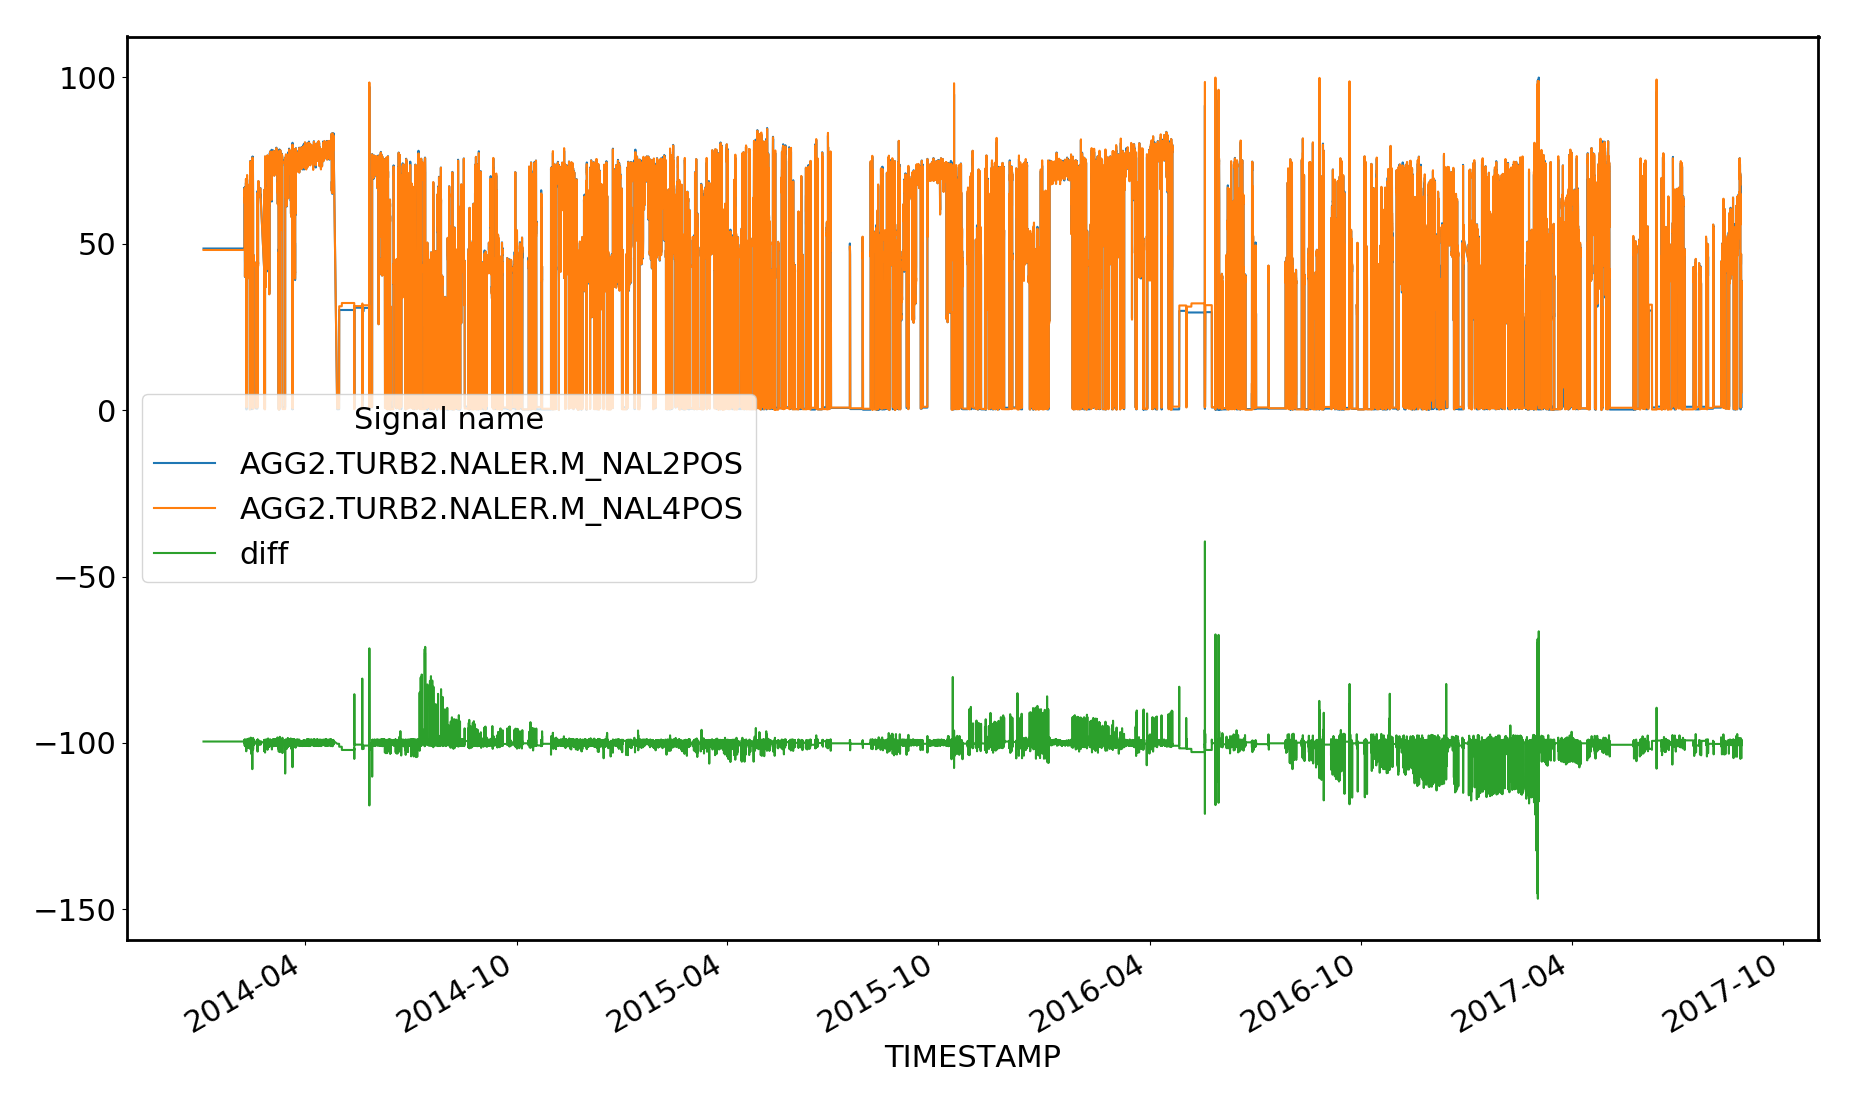
\includegraphics[width=\textwidth]{report/figures/data/turbine2_needle2_4.png}
            \caption{Needle 2 and 4 plotted on top of each other is seen in orange and blue at the top of the figure. With an offset of -100 the needle difference is seen in green. The dates are seen along the x-axis.}
            \label{fig:plant1_needle_error}
        \end{figure}
        
        
    \subsection{Other Pelton needle incidents}\label{subsec:start_failures}
        The log reported two other issues with the turbine needles at Plant $1$, that is observable in a scatter plot. This is seen in Figure \ref{fig:start_failure_turb1} and \ref{fig:start_failure_turb2}. Both are start-up failures due to problems with the needle operation.
        \begin{figure}[h!]
            % \caption*{Start up errors}
            \begin{minipage}[b]{0.49\linewidth}
                \centering
                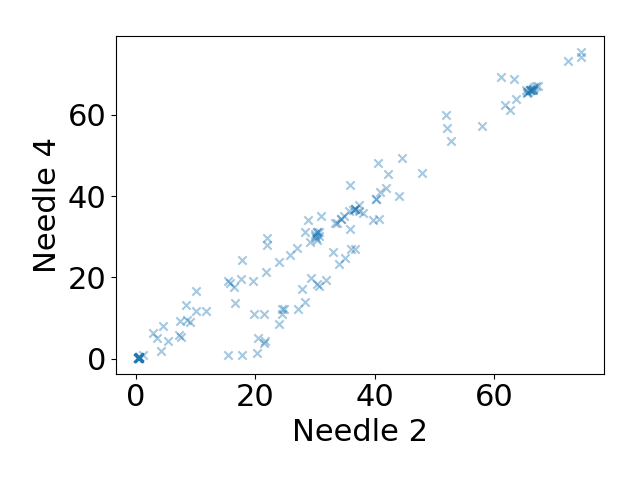
\includegraphics[width = \textwidth]{report/figures/data/turb1_n2_n4_scatter_start_failure_10122014.png}
                \caption{Turbine 1 start failure, 10.12.2014. Pairwise operated needles are scatterplotted against each other.}
                \label{fig:start_failure_turb1}
            \end{minipage}
            \hfill\vline\hfill
            \begin{minipage}[b]{0.49\linewidth}
                \centering
                \includegraphics[width = \textwidth]{report/figures/data/turb2_n1_n3_start_failure_25082016.png}
                \caption{Turbine 2 start failure, 25.08.2016. Pairwise operated needles are scatterplotted against each other.}
                \label{fig:start_failure_turb2}
            \end{minipage}
        \end{figure}
        
        
    
    \subsection{Other plants with Pelton turbines}
        Further investigation showed that the second plant with Pelton turbines also has two turbines with pairwise operated needles. The third Pelton plant only has one turbine, and the needles are not pairwise operated. The turbine use from 1 to 5 needles depending on the produced power. Data from this plant could be used to generalize the anomaly detection methods to handle any combination of needles, but this will not be covered in this thesis. The needle operation for the second plant is seen in Figure \ref{fig:plant2_needles}. One can see that turbine $1$ has no sampling on needle $1$, but the three other pairs are sampled correctly. Plant 2 further motivates that there is something wrong with the needles for plant $1$. All needle pairs follow the linear pattern much better and have very few anomalies.
        \begin{figure}
            \begin{minipage}[b]{0.5\linewidth}
                \centering
                \includegraphics[width=\textwidth]{report/figures/data/p2_t1_n1_n3.png}
            \end{minipage}
            \begin{minipage}[b]{0.5\linewidth}
                \centering
                \includegraphics[width=\textwidth]{report/figures/data/p2_t1_n2_n4.png}
            \end{minipage}
            \begin{minipage}[b]{0.5\linewidth}
                \centering
                \includegraphics[width=\textwidth]{report/figures/data/p2_t2_n1_n3.png}
            \end{minipage}
            \begin{minipage}[b]{0.5\linewidth}
                \centering
                \includegraphics[width=\textwidth]{report/figures/data/p2_t2_n2_n4.png}
            \end{minipage}
            \caption{Needle openings for the pairwise operated needles for both turbines at Plant 2 are scatterplotted in four sub-figures.}
            \label{fig:plant2_needles}
        \end{figure}
        
        
        
    % \section{Other process signals}
        
    
        
    %     mention that this alone is a case one can build upon but track the error to other process-variable would be very interesting both for condition monitoring but also for identification of the fault and why it happened. 
        
        
    %     It is important to understand that an outlier in the data does not necessarily mean that something is about to break. There is a possibility that the sample is an indication of a condition change in the equipment, but it might also be due to an error in the measurement, noise or just a deviation in the ongoing process. This makes this kind of analysis even harder. An outlier might be coincident, that yields little to no information. 
        
         
         
    \subsection{Artificial needle error}\label{subsec:arti}
        Due to not having any incidents similar to the one seen at plant 1 turbine 2, an artificial error replicating the error is created. The primary motivation is to see when an error that is increasing over time is detectable. A subset of the data sampled at plant 2 is altered to replicate an error similar to the one seen for plant 1. By doing so, one knows exactly when the error starts occurring. This can then be used to evaluate how early different anomaly detection techniques detect anomalies.
    
        The turbine needles are controlled through a hydraulic system. A hydraulic system can suffer from many problems which can cause operational problems, such as pressure drops due to both external and internal leakage. External leakage is often broken hoses or pipes. Internal leakages are within the pumps and actuators. Both types of leakages reduce the system pressure and can slow down the motion of the system. Oil contamination can also be an issue if filters are not maintained at a given interval, unfiltered oil can then lead to clogged components, which can lead to pressure drops. The leading theory of the problems seen at plant 1 is that the oil flow is restricted in one direction. As needle 4 closes, the larger the differential pressure caused by the water head being restricted becomes. As the differential pressure grows, closing the needle requires more force. This means that if the hydraulic system is suffering from reduced capacity in one direction, the motion of the needle will slow down as the needle close. 
        
        Figure \ref{fig:plant2_arti_error} shows the colored scatter plot for the plant 2 data with and without the artificial error. As can be seen, it has a very similar pattern to what was seen at plant 1 in the days leading up to the reported incident. Figure \ref{fig:plant2_arti_error_40}, shows a close up on the lower openings of the needle. The deviation between the two needles increases with time, as seen in the case of plant 1. The artificial error is added to data sampled from needle pair [2,4] on turbine 2 at Plant 2. Data from 20161001 to 20170401 is used, and the artificial error is added from 20170201.     
        
        \begin{figure}
            \begin{minipage}[b]{0.5\linewidth}
                \centering
                \includegraphics[width = \textwidth]{report/figures/analysis/artificial error/original_data_small.png}
                % \caption{Original data}
                % \label{fig:plant2_arti_orig}
            \end{minipage}
            \begin{minipage}[b]{0.5\linewidth}
                \centering
                \includegraphics[width = \textwidth]{report/figures/analysis/artificial error/plant2_arti_error_small.png}
                % \caption{Added artificial error}
                % \label{fig:plant2_arti_error}
            \end{minipage}
            \caption{Colored scatter plot of the data before and after adding the artificial error. The original data is seen in to the left. How to interpret the figure can be found in Figure \ref{fig:plan1_scatter_20161001-20170304}.}
            \label{fig:plant2_arti_error}
        \end{figure}
        
        \begin{figure}
            \centering
            \includegraphics[width = \textwidth]{report/figures/analysis/artificial error/plant2_artificial_error_scatter_colored_40.png}
            \caption{Colored scatterplot of the artificial error for the lower openings. How to interpret the figure is found in Figure \ref{fig:plan1_scatter_20161001-20170304}.}
            \label{fig:plant2_arti_error_40}
        \end{figure}
%!TEX root = ../Thesis.tex
\chapter{Results}\label{cha:analysis}
This chapter contains the anomaly detection analysis performed on the data presented in \ref{sec:pelton_needles}. The goal is to investigate how well different methods detect anomalies when only being exposed to normal data during training. Three anomaly detection techniques are used, OC SVM, KDE and LSTM RNN. First, the different training sets and test cases are presented, then some prepossessing steps are introduced before the optimal hyperparameters of the different methods are presented. Finally, the performance of the different methods on the different cases is presented.

    \section{Training sets and test cases}
        Due to the aperiodic sampling of process signals, only the needle positions are sampled often enough to be included as features in the analysis. This means that the techniques for feature and dimensionality reduction presented in chapter \ref{cha:litterature} will not be used. The anomaly detection techniques are trained on three different training sets and evaluated on four test cases. The goal is to analyze how the methods evaluate the different cases when trained on different training sets. 
        
        \begin{table}[]
            \centering
            \begin{tabular}{ccccccc}
                \toprule
                \textbf{Set}    & \textbf{Plant}       & \textbf{Needle}   & \textbf{Train}  & \textbf{Validation}        & \textbf{T. samples}\\ \midrule
                1       & 1                    & 2,4        & 20170304-20170701 & 20170701-20170825 & 9449\\ 
                2       & 2                    & 2,4        & 20160422-20160506 & 20160506-20161001 & 12870\\ 
                3       & 2                    & 2,4        & 20160101-20160506 & 20160506-20161001 & 84263\\ \bottomrule
            \end{tabular}
            \caption{Table over the three different training sets}
            \label{tab:training_cases}
        \end{table}
        
        The three different training sets are presented in Table \ref{tab:training_cases}. Training set 1 is from Plant 1 turbine 2 after the reported incident when the needle operation is back to normal. There is no golden rule for the ratio between testing and validation, but according to \cite{Kohavi1995} somewhere around $1/3$ of the data is common to use for validation. Only seven months of data is available from Plant 1 turbine 2 after the needles are fixed. Therefore five months are used as training data and little under two months for validation. This resulted in a training set of 9449 samples. The validation data is used to ensure that the methods are not overfitting on the training data. Training set 2 and 3 are taken from Plant 2 turbine 2, which has no reported incidents and normal system operation over the entire sample period. Set 2 is similar to set 1 in size, set 3 is 10 times larger. This is done to evaluate if the performance of the anomaly detection techniques changes when exposed to more or less data during training. The same data is used for validation for both sets. The validation data is larger simply because there is more data available. Data from 2016 was picked because it represented all operational modes well. 
        
        \begin{table}[]
            \centering
            \begin{tabular}{ccccc}
                \toprule
                \textbf{Case}    & \textbf{Plant} & \textbf{Turbine}   & \textbf{Needle pair}   & \textbf{Data}               \\ \midrule
                1       & 1     & 2         & 2,4           & 20140101-20170304     \\ 
                2       & 2     & 2         & 2,4           & 20161001-20170401     \\ 
                3       & 1     & 1         & 2,4           & 20140801-20150201     \\ 
                4       & 1     & 2         & 1,3           & 20160601-20161101     \\ \bottomrule
            \end{tabular}
            \caption{Table over the four different test cases}
            \label{tab:test_cases}
        \end{table}
        
        Table \ref{tab:test_cases} shows the four test cases. The first case is all data from Plant 1 turbine 2 up until the incident, as the data after is used for training. As this is the needle pair with the recorded incident, it is interesting to see how the different methods evaluate the data, especially building up towards the incident. Case 2 is the artificial case introduced in \ref{subsec:arti} where an artificial error is added to normal data from plant 2. The artificial error is added from 20170201. Hence, all data from 2016 is normal plant data. The artificial case enables one to evaluate how early the methods detect anomalies when knowing exactly the start date of the system degradation. Case 3 and 4 are data surrounding the reported start failures introduced in \ref{subsec:start_failures}. The start-up failures will help evaluate how well the methods recognizes known abnormal patterns in the data. 
        
        Training and evaluating the methods on data from different plants and turbines enables one to evaluate cross plant performance. This is very interesting, if it can be shown that one can simply deploy a pre-trained anomaly detection system at new plants with little to no alteration, this will greatly reduce the cost of installing such systems. 
        
        
        
    \section{Prepossessing steps}
        The data needs to be preprocessed before it can be analyzed. First, all time steps where not both needles are sampled are removed. Secondly, \cite{Tarassenko2009} talks about the importance of removing steady-state samples from the dataset, to avoid biasing the data.  The needles are constantly changing during operation, hence the only steady state is when the plant is not operating. Steady state is removed by removing all samples where the process signal values are close to zero ($<2$) and unchanged since the last sample. Having a stationary time series is important. As \cite{Manuca1996} explains, many of the common techniques for analyzing time series assume that the given series is stationary. A stationary time series is said to be independent of time, and don't have any correlations with seasonality. As the no operation data is removed from this dataset, the data is seen as stationary. The next step is to scale the data. For OC SVM and KDE, the data is scaled to zero mean and unit variance, for the LSTM RNN the data is scaled within a range of [0,1]. This was found to yield the optimal behavior for the different algorithms. To enable cross testing between plants, the transformations are calculated on plant 1 turbine 2 needles [2,4] and used for all datasets. Finally, the data is checked for outliers using scatterplots, as having anomalies in the training data could damage the systems ability to detect anomalies. 
    
    \section{Hyperparameterization}
        The methods chosen for the anomaly detection have several different parameters or hyperparameters. To ensure that the methods perform optimally, it is necessary to search for the best combination of these parameters. To enable comparing the different cases analyzed, an optimal parameterization is found and used for all cases. The hyperparameter search is performed on the data sampled from plant 1 turbine 2 needle [2,4], after the reported incident. 
            \subsection{One class support vector machine}
                The OC SVM has two tunable parameters. These are $\gamma$ and $\nu$. There is, however, no good way to automatically find the optimal parameterization for unlabeled data. By default, one has to inspect the one class SVM performance for different hyperparameterizations manually. It is attempted to create a custom cost function for automatic hyperparameterization. The cost function builds upon the idea that a good separating hyperplane or decision boundary lay close to the samples. The OC SVM implementation in scikit-learn stores the signed distance from each sample to the separating hyperplane. The distance can be used to evaluate the shape of the decision boundary. The proposed cost function is seen in equation \ref{eq:svm_cost} where $\bm{x}$ is the vector with the signed distances for each sample to the separating hyperplane. Several setups for a cost function were tried. The chosen performed well for the cases studied in this thesis. One cannot guarantee that it will perform adequately for different cases.  
                
                \begin{align}
                    \score = 1 - \abs(\std(\bm{x})) - \abs(\mean(\bm{x})) -\frac{\outliers}{\inliers}100
                    \label{eq:svm_cost}
                \end{align}
            
                As explained in theory, $\nu$ is the upper boundary for the fraction of outliers. Since the data is assumed to be outlier free, it is natural to pick values for $\nu$ that lie around $\frac{1}{N}$ where $N$ is the number of samples. $\gamma$ is a measure of the complexity of the decision boundary and is therefore chosen to span a wide range of values. A grid search is performed over the values seen in the list below. 
                \begin{itemize}
                    \item $\gamma =  [0.01,0.05,0.1,0.2,0.4,0.8,1,2,4,8,16]$
                    \item $\nu = [\frac{1}{25N}, \frac{1}{10N},\frac{1}{5N},\frac{1}{2N},\frac{1}{N},\frac{2}{N},\frac{5}{N},\frac{10}{N}]$
                    \label{list:svm_grid}
                \end{itemize}
                
                \begin{table}[h]
                    \centering
                    \begin{tabular}{ccc}
                        \toprule
                         \textbf{Score}  &   $\bm \gamma$    & $\bm \nu$         \\ \midrule
                         0.975  &   $0.05$      & $\frac{1}{N}$ \\ 
                         0.970  &   $0.1$      & $\frac{1}{2N}$ \\ 
                         0.961  &   $0.1$      & $\frac{1}{N}$ \\ 
                         0.960  &   $0.05$      & $\frac{2}{N}$ \\ 
                         0.957  &   $0.2$       & $\frac{1}{N}$ \\ 
                         -44.437  &   $8$      & $\frac{1}{10N}$ \\ 
                         -51.780  &   $8$      & $\frac{1}{25N}$ \\ 
                         -57.461  &   $0.1$      & $\frac{1}{25N}$ \\
                         -71.082  &   $16$      & $\frac{1}{10N}$ \\ 
                         -506.263  &   $16$      & $\frac{1}{25N}$ \\ \bottomrule
                         
                    \end{tabular}
                    \caption{Table showing the five best and five worst scores for the gridsearch after optimal hyperparameters for the one class SVM. $N = $ number of samples.}
                    \label{tab:svm_gridsearch}
                \end{table}
                
                Table \ref{tab:svm_gridsearch} shows the score for the five best and five worst hyperparameterizations. It can be seen that a too low $\nu$ or a too large $\gamma$ yields the worst performance. Figure \ref{fig:svm_grid_best} shows the decision boundary for the classifier that scored the best with regards of the cost function defined in equation \ref{eq:svm_cost}. All samples located inside the red boundary line, are classified as normal, and points outside as anomalies. The boundary covers all samples with a reasonable distance from the samples. As can be seen, most of the support vectors are located at the upper and lower range of the samples, showing the importance of having training data that span the full operating range of the machinery. A couple of samples in the mid area are also picked as support vectors. This gives a relatively close, but smooth boundary. The boundary for the worst parameterization is seen in Figure \ref{fig:svm_grid_wors}, it is easily verified that the boundary is to complex, due to a large $\gamma$ and a very small $\nu$. The decision boundaries for the remaining classifiers seen in table \ref{tab:svm_gridsearch}, are found in appendix \ref{apendix:svm_grid}. It is verified that all of the high scoring classifiers have a similar shape of the decision boundary. Note that the plots are produced using the scaled data. 
                
                \begin{figure}
                        \centering
                        \includegraphics[width=0.7\textwidth]{report/figures/analysis/gridsearch/Novelty detection, 1, training, gamma = 0.05 nu = 1.0583130489998942e-05.png}
                        \caption{Decision boundary for the best scoring classifier. All observations inside the red boundary are classified as normal, all observations outside as anomalies. The support vectors are seen in orange crosses. The color outside the boundary indicates the distance to the separating hyperplane.}
                        \label{fig:svm_grid_best}
                        
                \end{figure}
                
                \begin{figure}
                        \centering
                        \includegraphics[width=0.7\textwidth]{report/figures/analysis/gridsearch/Novelty detection, -1 training, gamma = 16 nu = 4.233252195999577e-06.png}
                        \caption{Decision boundary for the worst classifier. How to interpret the figure is found in Figure \ref{fig:svm_grid_best}}
                        \label{fig:svm_grid_wors}
                \end{figure}
    
                
                
            \subsection{Kernel density estimation}
                The optimal hyperparameters for KDE were found using the built-in grid search method in scikit-learn. The different parameterizations are scored based on how well they replicate the distribution of the original data. As with OC SVM, KDE only has two parameters, bandwidth and kernel type. The bandwidth serves as a smoothing parameter, the higher the bandwidth, the smoother the density estimation will become. The KDE grid search was performed over a bandwidth from $[0,1]$ at $0.1$ steps, and with Gaussian, Tophat, Epanechnikov, Exponential, Linear and Cosine as kernels. The optimal parameter combination was found to be the Gaussian kernel with $0.1$ as bandwidth. 
                
                
            \subsection{Long short term memory recurrent neural network}
                A custom grid search for the optimal hyperparameterization for the LSTM network was created. As the network is trained to recreate the input, the Euclidean norm of the difference between predicted and real value is used to score the performance of the network. The models were trained on a training set and tested on a validation set. The different parameters are shown in the list below.  
                \begin{itemize}
                    \item Epochs $= 100$
                    \item Batch size $=[8,32,128,1024]$
                    \item Neurons $= [2,4,8,16,32,64,128,256]$
                    \item Layers $= [1]$
                \end{itemize}
                A preliminary search found that increasing the layer depth introduced overfitting, and therefore only one layer was included in the grid search. The network consists of an LSTM layer with the number of neurons found in the grid search. In addition, there is a dense linear layer that recreates the input. The shape of the input is as required by Keras, transformed into a 3 dimensional tensor with dimension [num\_samples,num\_features,1]. Table \ref{tab:lstm_gri} shows the score for the five best and five worst parameter combinations. The grid search is performed with a maximum number of epochs set to $300$. Early stopping is used to avoid overfitting, and the optimal number of epochs for each parameterization is seen in the Table \ref{tab:lstm_gri}. Figure \ref{fig:lstm_grid_error_best} and \ref{fig:lstm_grid_error_worst} shows the training history plots for the best and worst configuration of the LSTM. As can be seen, the worst configuration is stopped after five epochs due to an increasing error in the test prediction. This is typical for models with high variance, which are prone to model random noise in the training set. Looking into the parameters for this configuration one can see that the batch size is very small, meaning that the network weights are updated after only being exposed to a small number of samples, this seems to cause overfitting. The best configuration is not stopped before it reaches 134 epochs, and as can be seen, it performs equally on both training and test data. The history plots for the eight other configurations can be found in appendix \ref{appendix:lstm_grid}. 
                
                
                % As can be seen the network performs best with one layer and a large number of neurons, the most important parameter seems to be the batch size, where smaller batch sizes outperform larger. Figure \ref{fig:lstm_grid_error_best} shows the model error for the optimal LSTM structure. As can be seen, the error gradually decrease towards 50 epochs,  but as it goes beyond, it can seem like there is a tendency to overfitting on the training data, as the test performance is changing, the training will, therefore, be stopped after 50 epochs. Figure \ref{fig:lstm_grid_worst} shows the model error for the worst parameterization. As can be seen, it performs a ten factor poorer than the best. Notice, however, that the model error is not converging, and hence the parametrization was tested by running for 300 epochs. Figure \ref{fig:lstm_worst_300} shows the result, as can be seen it converges, but still 
                
                \begin{table}[]
                    \centering
                    \begin{tabular}{ccccc}
                        \toprule
                        \textbf{Score}       & \textbf{Epochs}    & \textbf{Batch size}    & \textbf{Neurons}   & \textbf{layers}   \\ \midrule
                        $3.516e-03$     & $134$     & $256$          & $64$     & 1        \\ 
                        $3.521e-03$     & $288$     & $512$          & $16$      & 1        \\
                        $3.571e-03$     & $300$     & $1000$          & $64$      & 1    \\ 
                        $3.646e-03$     & $300$     & $1000$         & $128$      & 1   \\ 
                        $3.650e-03$     & $300$     & $256$         & $128$     & 1  \\ 
                        $0.026$         & $12$     & $16$          & $2$      & 1     \\
                        $0.026$         & $6$     & $16$        & $128$       & 1    \\ 
                        $0.026$         & $6$     & $16$        & $256$       & 1       \\ 
                        $0.031$         & $9$     & $8$          & $16$     & 1          \\
                        $0.046$         & $6$     & $8$          & $256$     & 1      \\ \bottomrule
                    \end{tabular}
                    \caption{Top five and bottom five scores after the grid search for optimal LSTM structure and parameters, the lower score the better the performance.}
                    \label{tab:lstm_gri}
                \end{table}
                
                \begin{figure}
                    \begin{minipage}[b]{0.49\linewidth}
                        \centering
                        \includegraphics[width = \textwidth]{report/figures/analysis/lstm_gridsearch/best_lstm_error_zoomed.png}
                        \caption{Training history for the best LSTM configuration. Test and training prediction error is shown as a function of epochs.}
                        \label{fig:lstm_grid_error_best}
                    \end{minipage}
                    \hfill\vline\hfill
                    \begin{minipage}[b]{0.49\linewidth}
                        \centering
                        \includegraphics[width = \textwidth]{report/figures/analysis/lstm_gridsearch/worst_lstm_error_-1.png}
                        \caption{Training history for the worst LSTM configuration. Test and training prediction error is shown as a function of epochs.}
                        \label{fig:lstm_grid_error_worst}
                    \end{minipage}
                \end{figure}
        
    \section{Anomaly detection}
        Of the three methods used in the analysis, only OC SVM is a classifier. KDE and LSTM RNN gives an anomaly score. Hence they will be referenced as anomaly scorers. This means that to identify a sample as an anomaly, one needs to find a threshold for the anomaly score. This is not covered in the thesis.
        
    \subsection{Training set 1, test case 1 and 2}
        \begin{figure}
            \centering
            \includegraphics[width=\textwidth]{report/figures/analysis/plant1_training/training_data_anomaly.png}
            \caption{Training set 1 with the anomaly results for the different methods. The upper subplot shows the needle openings on top of each other. The second subplot shows how the LSTM anomaly scorer evaluates the data seen in the upper subplot, the higher the score, the more anomalous the data is. The third subplot shows the KDE scorer, the more negative the score is, the more anomalous the data is. The orange line in the two score plots indicates the 0.1\% most extreme scores. The last subplot shows how the OC SVM classifies the needle openings, normal = 1 and anomalous = -1.}
            \label{fig:anomaly_training_set1}
        \end{figure}
        Figure \ref{fig:anomaly_training_set1} shows training set 1, and how the different methods evaluate the training data. As can be seen, the anomaly scores for the KDE and LSTM anomaly scorers are similar in shape but different in magnitude. One data point is standing out from the rest for all three methods, but the anomaly score is still very close to the average. The same point is also evaluated as an anomaly for the OC SVM classifier.
        
        \begin{figure}
            \centering
            \includegraphics[width = \textwidth]{report/figures/analysis/plant1_training/production_data_anomaly.png}
            \caption{Anomaly results for the methods trained on training set 1 and evaluated on test case 1. For plot interpretation see Figure \ref{fig:anomaly_training_set1}.}
            \label{fig:anomaly_plant_1_train_production}
        \end{figure}
        Figure \ref{fig:anomaly_plant_1_train_production} shows the anomaly scores for the three different methods on test case 1. The top window shows the opening of the two needles. As can be seen, it is hard to spot any deviation between the two needles, even for the data from the reported incident at the end of the plot. For both the KDE and the LSTM anomaly scorers one can clearly see that the anomaly score of the data is increasing from September 2016. Several samples after January 2017 are located above the proposed threshold line. The anomaly score for both scorers is more than doubled from the score seen during the lowest periods. This shows that one can clearly identify that the scorers are detecting patterns in the data not seen during training, in the period leading up to the incident. This is verified by comparing the magnitude of the anomaly scores from figure \ref{fig:anomaly_training_set1} and \ref{fig:anomaly_plant_1_train_production}. Interestingly, there are also several samples spread out over the entire sampling period that is given a high anomaly score. This can be because the training set does not cover all modes of operation, operational problems or problems with data sampling. This trend is also seen in Figure \ref{fig:plant1_needle_error}. The power plant log did not report any operational issues except for the one in March 2017, but from the authors experience from the industry, it is not uncommon that not all maintenance work is logged. The OC SVM classifier is not able to detect a trend towards the incident. As can be seen, it only evaluates a few anomalies in the period up until the reported incident. There are also signs of abnormalities earlier in the production data as seen for the anomaly scorers. Interestingly, one can see that the samples evaluated as anomalies for the one class SVM are all among the highest scoring samples for the two anomaly scorers. 
        
        Table \ref{tab:trainining_plant1_stats} shows how the scorers evaluate the validation data compared to the data from test case 1. The plot for the anomaly scores of the validation set can be found in appendix \ref{appendix:training_case1}. In addition, boundary plots for the SVM classifier, KDE scorer and learning history plots for the LSTM scorer can be found there. As can be seen, there is a large difference between the minimum value for the validation and case data for the KDE scorer. There is also a difference between the mean values. This shows that the test case 1 data takes on patterns not seen in the validation data. The same trend is seen in the statistics for the LSTM scorer. In both cases, the most extreme observation between training and production is approximately 100 times larger.
        
        Figure \ref{fig:svm_1_outliers_stats_production} shows the number and percentage of anomalies for the OC SVM classifier for test case 1. As can be seen, the anomaly percentage of the anomalies detected in 2014 and 2016 is much lower than for the reported incident in 2017. This indicates that separating what could be false positives from true positives, could be solved by using an anomaly percentage threshold. 
        
        \begin{table}[]
            % \begin{minipage}[b]{0.48\linewidth}
            \centering
            \begin{tabular}{ccccc}
                \toprule
                            & \textbf{KDE validation}  & \textbf{KDE case 1}    & \textbf{LSTM validation} & \textbf{LSTM case 2}   \\ \midrule
                min         & -2.671    & -275.66           & 1.659e-04 & 9.716e-05         \\ 
                max         & 0.491     & 0.491             & 3.032e-2  & 0.400             \\ 
                mean        & -0.296    & -0.728            & 3.318e-03 & 6.200e-3          \\ \bottomrule
            \end{tabular}
            \caption{Table comparing the statistics for the KDE and LSTM anomaly detectors on the validation and case 1 data for training case 1}
            \label{tab:trainining_plant1_stats}
        \end{table}
        
        \begin{figure}
            \begin{minipage}[b]{0.49\linewidth}
                \centering
                \includegraphics[width=\textwidth]{report/figures/analysis/plant1_training/daily_svm_outliers_production_small.png}
                \caption{Daily classified anomalies for the one class SVM classifier on production data}
                \label{fig:svm_1_outliers_stats_production}
            \end{minipage}
            \hfill\vline\hfill
            \begin{minipage}[b]{0.49\linewidth}
                \centering
                \includegraphics[width=\textwidth]{report/figures/analysis/plant1_training/daily_svm_outliers_artificial_small.png}
                \caption{Daily classified anomalies for the one class SVM classifier on artificial data}
                \label{fig:svm_1_outliers_stats_artificial}
            \end{minipage}
        \end{figure}
        
        Figure \ref{fig:anomaly_plant_1_train_artificial} shows the anomaly scores for test case 2. Note that test case 1 and 2 are from different plants. There is no sample data from January 2017, but since dates are used as indexes, January is still seen in the plot. The data from 2016 is normal data from plant 2, and the artificial error is gradually increasing from February to April in 2017. As can be seen, both the LSTM and KDE scorers have growing anomaly scores from mid-February. Towards March, the anomaly scores are significantly higher than for the normal data. Looking at figure \ref{fig:anomaly_plant_1_train_production} one can see that the anomaly score for the artificial error is of the same magnitude as the score for test case 1 in the months before the incidents. 
        
        The OC SVM classifier is not picking up the trend as fast as, but it clearly detects that something is wrong towards the end of the sample period. This can be verified by looking at \ref{fig:svm_1_outliers_stats_artificial}. Notice however how few samples that are classified as anomalous, and that the percentage is very low.      
        \begin{figure}
            \centering
            \includegraphics[width = \textwidth]{report/figures/analysis/plant1_training/artificial_data_anomaly.png}
            \caption{Anomaly results for the methods trained on training set 1 and evaluated on test case 2. For plot interpretation see Figure \ref{fig:anomaly_training_set1}.}
            \label{fig:anomaly_plant_1_train_artificial}
        \end{figure}
    
    \subsection{Training set 2, test case 1 and 2}
        \begin{figure}
            \centering
            \includegraphics[width=\textwidth]{report/figures/analysis/plant2_train_short/training_data_anomaly.png}
            \caption{Anomaly results for the methods trained on training set 2 evaluated on training set 2. For plot interpretation see Figure \ref{fig:anomaly_training_set1}.}
            \label{fig:anomaly_training_set2}
        \end{figure}
        Figure \ref{fig:anomaly_training_set2} shows training set 2, and how the different methods evaluate the training data. As can be seen the anomaly scores for the KDE and LSTM anomaly scorers are not as similar in shape as was seen for training set 1. They are also reduced in magnitude. The OC SVM evaluates all data points as normal. 
    
        \begin{figure}[h!]
            \centering
            \includegraphics[width=\textwidth]{report/figures/analysis/plant2_train_short/production_data_anomaly.png}
            \caption{Anomaly results for the methods trained on training set 2 and evaluated on test case 1. For plot interpretation see Figure \ref{fig:anomaly_training_set1}.}
            \label{fig:plant2_short_prod_anomaly_score}
        \end{figure}
        Figure \ref{fig:plant2_short_prod_anomaly_score} shows the anomaly scores for test case 1, when training the methods on training set 2. Training set 1 and 2 are as mentioned approximately of the same size. The figure shows a very similar pattern for the two anomaly scorers to what was seen for training set 1. This could mean that both methods generalize well across plants, at least as long as the training sets are of similar size. 
        
        The biggest difference is seen in the OC SVM window, where some new samples are being classified as anomalies in 2015. This could show that OC SVM is more sensitive to the training data, as the data from 2015 seems to be the best data from this needle pair. However, looking at Figure \ref{fig:svm_2_outliers_stats_production} it becomes clear that the number of anomalies detected in 2015 is small, and that setting a threshold as mentioned in the previous section could classify them as false positives.  
        
        Table \ref{tab:trainining_plant2_short_stats} shows the anomaly statistics for the validation set and test case 1. It is clear that both scorers have a higher minimum and maximum values than what was seen when the methods were trained on training set 1. They are, however, very similar in magnitude. The mean values for both scorers are also changed, which could indicate that the score is simply biased. 
        \begin{table}[]
            \centering
            \begin{tabular}{ccccc}
                \toprule
                            & \textbf{KDE validation}  & \textbf{KDE case 1}     & \textbf{LSTM validation}     & \textbf{LSTM case 1}   \\ \midrule
                min         & -4.566        & -296.370           & 2.336e-05            & 2.336e-05         \\ 
                max         & 1.291         & 1.2905             & 4.047e-2             & 0.498             \\ 
                mean        & --0.518       & -1.493             & 4.976e-04            & 8.116e-3          \\ \bottomrule
            \end{tabular}
            \caption{Table comparing the statistics for the KDE and LSTM anomaly detectors on the validation and production data}
            \label{tab:trainining_plant2_short_stats}
        \end{table}
        \begin{figure}[h!]
            \begin{minipage}[b]{0.49\linewidth}
                \centering
                \includegraphics[width=\textwidth]{report/figures/analysis/plant2_train_short/daily_svm_outliers_production_small.png}
                \caption{Anomaly statistics for OC SVM on production data}
                \label{fig:svm_2_outliers_stats_production}
            \end{minipage}
            \hfill\vline\hfill
            \begin{minipage}[b]{0.49\linewidth}
                \centering
                \includegraphics[width=\textwidth]{report/figures/analysis/plant2_train_short/daily_svm_outliers_artificial_small.png}
                \caption{Anomaly statistics for OC SVM on artificial data}
                \label{fig:svm_2_outliers_stats_artificial}
            \end{minipage}
        \end{figure}
        
        \begin{figure}[h!]
            \centering
            \includegraphics[width=\textwidth]{report/figures/analysis/plant2_train_short/artificial_data_anomaly.png}
            \caption{Anomaly results for the methods trained on training set 2 and evaluated on test case 2. For plot interpretation see Figure \ref{fig:anomaly_training_set1}.}
            \label{fig:plan2_short_arti_anomaly_score}
        \end{figure}
        Figure \ref{fig:plan2_short_arti_anomaly_score} shows the anomaly scores for the artificial data in test case 2. As with test case 1, both scorers behave very similar to what was seen for training set 1. Looking at the LSTM anomaly score in window two, one can verify that the anomaly score increases immediately after the error is applied. It can detect only small deviation from the normal operating pattern. The  KDE scorer also seems to pick up the artificial error faster than for training set 1. As the artificial error is added to process data from the same needle pair that is used for the data in training set 2, it is sensible that it is possible to detect the anomalies earlier than for training set 1. Looking at figure \ref{fig:plant2_short_prod_anomaly_score} one can see that the anomaly score for the artificial error is of the same magnitude as the score for test case 1 in the months before the incidents. 
        
        The OC SVM detector is, however, having problems detecting the anomalies, and only detects the sample that the two other detectors identify as the most anomalous. One possible explanation to this is that the parameters found in the hyperparameterization for the OC SVM do not generalize very well to new data, as the hyperparameterization was performed on data from plant 1. Figure \ref{fig:svm_2_outliers_stats_artificial} shows that the classifier is only classifying three samples as anomalous. The plot for the anomaly scores of the validation set can be found in appendix \ref{appendix:training_case2}, in addition, boundary plots for the OC SVM classifier, KDE scorer and learning history plots for the LSTM scorer can be found there.
        
        
    
    \subsection{Training set 3, test case 1 and 2}
        \begin{figure}
            \centering
            \includegraphics[width=\textwidth]{report/figures/analysis/plant2_train_long/training_data_anomaly.png}
            \caption{Anomaly results for the methods trained on training set 3 evaluated on training set 3. For plot interpretation see Figure \ref{fig:anomaly_training_set1}.}
            \label{fig:anomaly_training_set3}
        \end{figure}
        Figure \ref{fig:anomaly_training_set3} shows training set 3, and how the different methods evaluate the training data. The magnitude of the anomaly scores for the two scorers is between the scores for training set 1 and 2.  The OC SVM evaluates the most anomalies of all the training sets. As this training set is 10 times larger than the two other, this further strengthens the claim that the OC SVM hyperparameters are sensitive to the training data. 
    
        \begin{figure}[h!]
            \centering
            \includegraphics[width=\textwidth]{report/figures/analysis/plant2_train_long/production_data_anomaly.png}
            \caption{Anomaly results for the methods trained on training set 3 and evaluated on test case 1. For plot interpretation see Figure \ref{fig:anomaly_training_set1}.}
            \label{fig:plant2_lomg_prod_anomaly_score}
        \end{figure}
        Figure \ref{fig:plant2_lomg_prod_anomaly_score} shows the anomaly scores and classifications for test case 1 when trained on training set 3. The scorers evaluate anomalies very similar to what was seen for training set 1 and 2. Both scorers detect a rising trend of abnormal data towards the reported incident in March 2017. The anomaly scores for the data from the day of the incident is very high for both scorers, as was seen in the two previous cases as well. The OC SVM classifier is classifying test case 1 very similar to what was seen for training set 2, as is verified by Figure \ref{fig:svm_3_outliers_stats_production}. Adding more data from plant 2 did not fix the issue with what appears to be false positives in the data sampled in 2015. 
        
        \begin{figure}[h!]
            \begin{minipage}[b]{0.49\linewidth}
                \centering
                \includegraphics[width=\textwidth]{report/figures/analysis/plant2_train_long/daily_svm_outliers_production_small.png}
                \caption{Anomaly statistics for one class SVM on production data}
                \label{fig:svm_3_outliers_stats_production}
            \end{minipage}
            \hfill\vline\hfill
            \begin{minipage}[b]{0.49\linewidth}
                \centering
                \includegraphics[width=\textwidth]{report/figures/analysis/plant2_train_long/daily_svm_outliers_artificial_small.png}
                \caption{Anomaly statistics for one class SVM on artificial data}
                \label{fig:svm_3_outliers_stats_artificial}
            \end{minipage}
        \end{figure}
        
        Table \ref{tab:trainining_plant2_long_stats} show the statistics for the LSTM and KDE detectors, the statistics are similar to what was seen in the previous training sets. Early stopping stopped the LSTM scorer after only 20 epochs, where the two previous sets ran for 134. When running the LSTM for 134 epochs, the performance of the LSTM scorer was much worse than for the previous training sets. This could indicate that training set 2 holds the same information as training set 3, but as training set 3 has more samples, the algorithm does not need to iterate over the entire set as many times. Early stopping is used to avoid overfitting on the training data, and the poor performance when running for 134 epochs on set 3, is most likely due to overfitting. The fact that the two other methods appear to evaluate test case 1 similar for both training set 2 and 3, further strengthens this claim. If the added data in set 3 has a different distribution than the one in training set 2, this would have been caught by KDE and one class SVM.     
        \begin{table}[]
            \centering
            \begin{tabular}{ccccc}
                \hline
                            & \textbf{KDE validation}  & \textbf{KDE case 1}     & \textbf{LSTM validation} & \textbf{LSTM case 1}   \\ \midrule
                min         & -2.755    & -277.804              & 2.559e-05         & 2.796e-05         \\ 
                max         & 0.999     & 0.9995                & 3.597e-2          & 0.471             \\ 
                mean        & -0.366   & -1.167                 & 6.709e-04         & 7.651e-03          \\ \bottomrule
            \end{tabular}
            \caption{Table comparing the statistics for the KDE and LSTM anomaly detectors on the validation and production data}
            \label{tab:trainining_plant2_long_stats}
        \end{table}




        % Figure \ref{fig:plan2_short_arti_anomaly_score} shows the anomaly scores for the artificial data. As with the production data from plant 1 both the KDE and LSTM detectors behave very similar to what was seen for training case 1. Looking at the LSTM anomaly score in window two, one can verify that the detector can track the artificial error from the date it is applied whereas for training case 1 it took a long time before the anomaly score indicated something abnormal. The one class SVM detector is, however, having problems detecting the anomalies, and only detects the sample that the two other detectors identify as the most abnormal. Note that the training case here is based on normal data from plant 2. It seems like the parameters found in the hyperparameterization of the one class SVM does not generalize very well to new data.
        \begin{figure}[h!]
            \centering
            \includegraphics[width=\textwidth]{report/figures/analysis/plant2_train_long/artificial_data_anomaly.png}
            \caption{Anomaly results for the methods trained on training set 3 and evaluated on test case 2. For plot interpretation see Figure \ref{fig:anomaly_training_set1}.}
            \label{fig:plan3_long_arti_anomaly_score}
        \end{figure}
        Figure \ref{fig:plan3_long_arti_anomaly_score} shows the anomaly scores for test case 2. As for test case 1, one can verify that the scorers behave more or less equal to what was seen for training set $2$. The OC SVM classifier is detecting anomalies in the normal test data, and it is only able to classify data from one day during the artificial error as anomalous. Figure \ref{fig:svm_3_outliers_stats_artificial} shows that for a day in the end of December, all samples are evaluated as anomalies. This is most likely due to only one sample being stored right after midnight. The fact that training set 3 yields the poorest performance for the OC SVM, further strengthens the assumption that the algorithm is sensitive to the combination of hyperparameters and training data. The plot for the anomaly scores on the validation set can be found in appendix \ref{appendix:training_case3}, in addition, boundary plots for the SVM classifier, KDE scorer and learning history plots for the LSTM scorer can be found there.
        
    
    
    \subsection{Comparing the methods for all training sets, on test case 1}
        \begin{figure}[h!]
            \centering
            \includegraphics[width=\textwidth]{report/figures/analysis/training_cases/lstm_training_cases.png}
            \caption{The anomaly score for the three LSTM scorers tested on test case 1, is seen in the three lower subplots. The upper subplot shows the needle positions on top of each other. The orange line indicates the 0.1\% most extreme scores.}
            \label{fig:lstm_training_cases}
        \end{figure}
        To simplify comparing the performance of the different methods new plots are created that shows how the different methods evaluate the production data in test case 1, for all three training sets. Figure \ref{fig:lstm_training_cases} show how test case 1 is evaluated by the three LSTM scorers. It is clear that all the scorers perform very similar. This shows that the method works well for both large and smaller training sets. All scores indicate a growing anomaly trend towards the incident in 2017, but the scorers for training set 2 and 3 show an increasing anomaly trend earlier than the scorer for set 1. A theory for why this is happening is that the training data used in set 1 is sampled right after maintenance, while the training sets from plant 2 are sampled after years of operation. This means that minor deviations between the needles that could be normal after some time of use is seen as anomalous for the scorer trained on set 1 while this is seen as normal when set 2 and 3 are used for training. However, deploying any of the three scorers at the plant could have warned about an increase in anomalous observations, that could have identified the anomalous trend before it is becoming too extreme. 
        
        \begin{figure}[h!]
            \centering
            \includegraphics[width=\textwidth]{report/figures/analysis/training_cases/kde_training_cases.png}
            \caption{The anomaly score for the three KDE scorers tested on test case 1, is seen in the three lower subplots. The upper subplot shows the needle positions on top of each other. The orange line indicates the 0.1\% most extreme scores.}
            \label{fig:kde_training_cases}
        \end{figure}
        Figure \ref{fig:kde_training_cases} shows how the different KDE scorers compare. All three scorers evaluate test case 1 very similar. The scorer from training set 2 gives the highest anomaly scores for the data leading up to the incident. As with the LSTM scorers, set 2 and set 3 appears to perform slightly better than set 1. All three scorers are able to detect the growing number of abnormal data seen towards March 2017. Notice that the score is limited to -75 to enable the reader to see the smaller trends, as the extreme values go below -250, making interpreting the plot very hard.
        
        \begin{figure}[h!]
            \centering
            \includegraphics[width=\textwidth]{report/figures/analysis/training_cases/svm_training_cases.png}
            \caption{The anomaly classification for the three OC SVM classifiers tested on test case 1, are seen in the three lower subplots. The upper subplot shows the needle positions on top of each other. Normal data = 1, anomalous data = -1}
            \label{fig:svm_training_cases}
        \end{figure}
        Finally, Figure \ref{fig:svm_training_cases} show the three different one class SVM classifiers. As with the two previous methods, there is little difference between set 2 and 3. This is the only method that appears to perform best when trained on data from plant 1. However, there is very little difference in the classifications, and when using the percentage of daily anomalies, one can easily separate the data from the incident with the other. This method is harder to spot trends with, and with the current parameterization, it is hard to find a way this method can be used as an early warning system for the incident seen in March 2017. This makes sense, as this method predicts all data as either normal or anomalous, and hence include an extra step compared to KDE and LSTM, which gives a score that the user need to interpret. Hence using this method would require less of the user, but more tuning and testing to ensure correct behavior. 
        
    
    \subsection{Test case 3 and 4}
        As the production data from test case 1 only contained one reported anomaly, the methods are tested on two start failures in test case 3 and 4. The results for the methods trained on training set 2 is seen in Figure \ref{fig:start_up_t1} and \ref{fig:start_up_t2}. In Figure \ref{fig:start_up_t1} one can see that the reported start failure from 10.12.2014 is given a high anomaly score for both scorers. The OC SVM classifier is not able to detect the start failure, and also appears to classify data from November as an anomaly wrongly. Notice that the magnitude of the scores is lower than what was seen for the most extreme samples from test case 1, it is, however, very similar to the magnitude seen for the artificial error.
        \begin{figure}
            \centering
            \includegraphics[width=\textwidth]{report/figures/analysis/startup_errors/t1_n2_n4_startup_error_anomaly_score_2_long.png}
            \caption{Anomaly results for the methods trained on training set 2 and evaluated on test case 3. How to interpret the figure can be seen in Figure \ref{fig:anomaly_training_set1}.}
            \label{fig:start_up_t1}
        \end{figure}
        In Figure \ref{fig:start_up_t2}, the start failure from case 4 is analyzed. The scoreres evaluate the start failure to be more anomalous than the start failure in case 3, as the magnitude of the scores are doubled. This is reasonable when looking at Figure \ref{fig:start_failure_turb1} and \ref{fig:start_failure_turb2}, where the scatterplot for turbine 1 clearly deviates more than the scatterplot for turbine 2. The OC SVM classifer is also able to detect the start failure.
        \begin{figure}
            \centering
            \includegraphics[width=\textwidth]{report/figures/analysis/startup_errors/t2_n1_n3_startup_error_anomaly_score_2_long.png}
            \caption{Anomaly results for the methods trained on training set 2 and evaluated on test case 4. How to interpret the figure can be seen in Figure \ref{fig:anomaly_training_set1}.}
            \label{fig:start_up_t2}
        \end{figure}
        The figures for the two other training sets can be found in appendix \ref{appendix:startup_failure}. They are not included in this section, due to very similar performance as the one seen for training set 2. 
    
    
    
    
    
    
    
    
    
    
    
    
    
    
    
    
    
    
    
    
    %     \begin{figure}
    %         \centering
    %         \includegraphics[width=\textwidth]{report/figures/analysis/plant2_train_long/test_data_anomaly.png}
    %         \caption{Anomaly score for the plant 2 test set, detectors trained on plant 2 long training set}
    %         \label{fig:plant2_long_test_anomaly_score}
    %     \end{figure}
        
    %     \begin{figure}
    %         \centering
    %         \includegraphics[width=\textwidth]{report/figures/analysis/plant2_train_long/production_data_anomaly.png}
    %         \caption{Anomaly score for the plant 1 production set, detectors trained on plant 2 long training set}
    %         \label{fig:plant2_long_production_anomaly_score}
    %     \end{figure}
    
    
    
    %     % \begin{table}[]
    %     %     \centering
    %     %     \begin{tabular}{|c|c|c|}
    %     %         \hline
    %     %         Test        & KDE       & LSTM  \\ \hline
    %     %         min         & -2.755    & 4.024e-05 \\ \hline
    %     %         max         & 0.999    & 0.0024   \\ \hline
    %     %         mean        & -0.366   & 0.000223  \\ \hline
    %     %     \end{tabular}
    %     %     \caption{Table of statistics for the test data for plant 2 long detector}
    %     %     \label{tab:production_stats_plant1train}
    %     % \end{table}
        
    %     % \begin{table}[]
    %     %     \centering
    %     %     \begin{tabular}{|c|c|c|}
    %     %         \hline
    %     %         Production          & KDE       & LSTM  \\ \hline
    %     %         min                 & -277.804   & 2.013e-05 \\ \hline
    %     %         max                 & 0.9987    & 0.0.0457   \\ \hline
    %     %         mean                & -1.1697    & 0.0.000807  \\ \hline
    %     %     \end{tabular}
    %     %     \caption{Table of statistics for the production data for plant 2 long detector}
    %     %     \label{tab:production_stats_plant1train}
    %     % \end{table}

    %     \begin{figure}
    %         \centering
    %         \includegraphics[width = 0.5\textwidth]{report/figures/analysis/plant2_train_long/svm_daily_outliers.png}
    %         \caption{Outlier statistics for svm}
    %         \label{fig:svm_outliers_stats}
    %     \end{figure}
        
        
    
    % \clearpage
    % \subsection{Anomaly detection 3, artificial error}
    %     The anomaly detectors trained on plant 2 are tested on the artificial error created on data from plant 2 not used for training. 
    %     \begin{figure}
    %         \centering
    %         \includegraphics[width=\textwidth]{report/figures/analysis/plant2_train_4months/plant2_artificial_anomaly_datetime.png}
    %         \caption{Anomaly score for the detectors trained on the normal data from plant 2, tested on artificial error data. The red line marks the $1\%$ most extreme scores.}
    %         \label{fig:plant2_arti_anomaly_score}
    %     \end{figure}
        
    %     As seen in figure \ref{fig:plant2_arti_anomaly_score} the detectors clearly detect the artificial error. The error is as explained above constructed to increase its effect gradually, and all three detectors can detect this pattern. It also looks similar to the pattern seen for the production data from plant 1. This further strengthens the claim that the error reported in March 2017, could be traced in the needle operation from early fall 2016. The artificial error is added to production data for plant $2$ from $2015$. This means that it is not seen by the detectors since they are trained from production data from $2016$.  
        
        
        
        
    % not possible to use any time-series forecasting since the data is not sampled at even frequencies. hence using a regression model and estimating an anomaly based on differences from the sampled and predicted data becomes invalid. 
    
    % bruke kde men det vil antagelig ikkje gje gode resultat sidan samplinga mi er dårlig, og eg ikkje har nok data spredd godt nok utover tilstandsrommet. 

% \section{Unsupervised dimensionallity reduction}\label{sec:dim_reduc}

%     \subsection{PCA}\label{subsec:PCA}


%     \subsection{Kernel PCA}\label{subsec:K_PCA}
    


% \section{Pelton needles}\label{sub:pelton_needles}
%     As mentioned, there was data available from three different power plants with Pelton turbines. One of the plants had recorded several issues with the needle control and was used as a case to test early detection of problems with the needle operation. 
    
    
%     \begin{figure}
%         \centering
%         \includegraphics[scale=0.8]{report/figures/analysis/hjartdola/hjar_n2_4_novelty_05_1e-5_train.png}
%         \caption{OCSVM trained on data after overhaul in Mars 2017}
%         \label{fig:my_label}
%     \end{figure}


    
%     \begin{figure}
%         \centering
%         \includegraphics[scale=0.8]{report/figures/analysis/hjartdola/hjar_n2_4_novelty_05_1e-5_test.png}
%         \caption{All process data from before the overhaul}
%         \label{fig:my_label}
%     \end{figure}




%!TEX root = ../Thesis.tex
\chapter{Discussion}\label{cha:discussion}

\section{Analyzing the data and building a case}
    Before the data analysis could start, the data needed to be reconstructed. As mentioned the data was far from ready for analysis as it was received. A python library was created that automatically reads the files received by the energy company, and produces data with a structure that allows analysis. The library is created in a way that allows for easy use of new data in the same format. This shows one of several challenges when working with real-world data from the industry.    
    
    Several issues arose once starting working with the data. A problem which most likely is relevant to most industries today is that having data is far from a guarantee of having good data. At first glance, the 90Gb of available data seemed like more than enough find many interesting cases. However, as the work progressed, it became apparent that finding good cases for testing anomaly detection, was not straightforward. It became clear that very few variables were sampled simultaneously, at a higher rate than hourly. Due to this, much time was spent trying to find a case that did not need a higher sampling rate. Going through the plant logs, no good cases were found. It might be possible that the energy company is sampling data in a scheme similar to the one used in \cite{Selak2014}, but this is very hard to reverse engineer from the data. Even if one chooses to sample data in such a scheme, it would be beneficial to sample more data at a higher and constant frequency, as it could open up for using techniques such as time-series forecasting. 
     
    Going through the logs from the power plants, the Pelton needle case was quickly picked out as interesting. As \cite{Aasnes2017} focused on the guide vanes of Francis turbines, building a case around the Pelton needles would serve as a natural extension, where one of the methods used for the Francis case could be tested on a new case. The needles play a vital part in the power production, and increasing knowledge about their condition and the operational trend would be a great addition to the existing instrumentation. Having four different Pelton turbines from two different plants in the dataset would allow testing how much adaptation would be needed to make the different anomaly detection techniques work on new plants. Having turbines with no reported incidents also made it possible to verify if the techniques were prone to give false positives.  
     
    It would have been interesting to include more than just the needle variables in the analysis, but this was not possible due to the data. The methods used in the analysis can handle more variables. Hence the analysis can be extended if the data is available. The possibility of using interpolation to handle the missing data was also addressed, but it was quickly discarded as it would require a lot of plant and process insight to pick techniques that interpolated every  process variable in a reasonable way.     
     
     As there only was one reported incident with the needles during operation, it was decided to create an artificial error that replicates the needle pattern seen for the days building up to the incident. Having the start date of the artificial error would give an insight into how quickly the anomaly detection techniques can catch such a trend. It could also give an indication of when one could expect that the original error started.  
    
    
  

\section{Choosing the methods}
    Several different anomaly detection methods and techniques were considered. As the Pelton case only had one reported incident, it made making a labeled data set hard. This opted for using methods that did not need labeled data, as one does not have to collect data from all the known failure modes, only from normal operation. As mentioned in the introduction, this opens the possibility also to detect unknown failure modes. This means that methods for labeled and unlabeled data does not exclude one another, and for a complete condition monitoring system using both approaches might yield the best solution. Three methods were chosen for the anomaly analysis, that all have been used for anomaly detection. OC SVM was chosen because it showed promise in the case with the Francis turbines guide vanes. KDE was picked because it is a relatively simple method, which is fast to implement through scikit-learn. The LSTM RNN algorithm was picked because it has shown promise when working with time series, and would serve well for comparison for the less complex other methods. Where OC SVM is a classifier, KDE and LSTM RNN are regressors. Hence the two latter does not classify the data as normal or abnormal. They produce a score that mirrors how anomalous the data is evaluated to be.
    
\section{Hyperparameterization}
    The optimal set of hyperparameters were searched for through a grid search for the three methods. The parameters were found using data from plant 1, and the same parameters were used for all the different training sets. This was done to see how well the methods would transfer between plants. If one needs to search for the optimal hyperparameters for each plant, then it will not be possible to deploy a pre-trained anomaly detection system simply. KDE and LSTM RNN was found to adapt well to data from new plants. A more extensive search for the optimal set of hyperparameters could have been performed, especially for OC SVM and LSTM RNN, but as the goal of this thesis was to investigate possible anomaly detection methods, the parameterizations found yielded good enough results to give an indication on what the methods can be used for.
    
    The custom cost function designed for the one class SVM seemed to work as intended, but can most likely be improved. As one gets more knowledge about how the data is structured, using different kernels, then the Gaussian kernel can also help with the performance of the algorithm.

\section{Training sets and test cases}
    Many different approaches could have been taken with the training sets and test cases. The main motivation for the chosen setup was that it enabled to compare performance across plants and training sizes. Many more cases could have been created, but as mentioned earlier this is an initial study, that can be used as starting ground for further testing. It was clear that the sampling rate was very different between the plants, as 14 days of sampling on plant 2 gave as many data points as almost five months at plant 1. This shows the importance of investigating the data. It was also important to ensure that the 14 days from plant 2 covered all operational modes for the plant. The final setup was three different training sets and four different test cases. The three training sets made it possible to evaluate how well the methods adapted to data from different plants and of different sizes. As it was chosen to use the optimal hyperparameterization found for data from plant 1, it also gave insight into how general the parameters were. The artificial test case made it possible to evaluate the performance of the production data seen in test case 1. The two start failure cases made it possible to evaluate the performance of more than one reported incident. 


\section{Performance of the methods}
    All methods showed promise in detecting the reported incident from plant 1 found in test case 1. OC SVM performed best when trained on training set 1. This indicates that the method is more sensitive to the chosen hyperparameters and that the optimal hyperparameters change when the training set changes. It also became clear that the OC SVM did not catch the pattern building up to the reported incident in test case 1, and that it seems like a method more suited for shutdown alerts than for early warning. As the method is trained without labeled data, it is hard to find the optimal selection of hyperparameters. The custom cost function created tried to deal with this issue, but as can be seen from the performance, there could be a set of hyperparameters that would increase the performance of the OC SVM. When the method was trained on data from plant 2, it showed signs of giving false positives. This further strengthens the claim that the optimal hyperparameters change when the training set is changed. 
    
    KDE and LSTM RNN performed very similarly for all training sets on all test cases. This indicates that the two methods are more robust to changes in the training set. It is, however, important to notice that the LSTM RNN needed early stopping to yield a similar performance from training set 3. Complex NNs always run the risk of overfitting to the data. Both methods performed best when trained on training set 2. As mentioned in the analysis this can be because training set 2 is taken from plant 2 after years of operation, and it might then better represent normal needle deviation, not seen in the training set from plant 1 sampled right after maintenance. In addition set 2 is approximately of the same size as set 1 which the hyperparameterization is performed on, where as set 3 is 10 times larger. This shows that even if KDE and LSTM RNN seem more robust to changing the training sets without changing the hyperparameterization, this still is a concern one needs to keep in mind. Both methods clearly evaluated the data from the reported incident in test case 1 as anomalous, and one could identify a growing trend in the anomaly score towards the incident.   
    
    The artificial error in test case 2 showed that both KDE and LSTM RNN could detect an error as the one seen in plant 1 in its early stages. For training set 2, the LSTM RNN showed an increase in the anomaly score immediately after the artificial error was added to the data. The KDE also found this pattern but did not detect it as fast. This means that it is likely that the pattern seen for the anomaly scores for test case 1 towards the reported incident, can be used as an early warning system for system degradation. One can also claim that it can be detected by a pre-trained method, as long as the same transformation is used for both training and test data.  
    
    % One class SVM started to indicate anomalies one month before the peak when trained on training set 1. For training set 2 it only detected the sample that was evaluated as most anomalous by the two other methods. For training set 3 it also started gave false positives. This further strengthens the claim that the method is very sensitive to changes in training data and that the optimal hyperparameters for the method are strongly connected to the structure of the training data. KDE and LSTM RNN showed that pre-trained methods can be deployed to a new plant, and still perform on a high level. They also showed that even if they seem robust, the hyperparameters are connected to the training data. 
    
    Training case 3 and 4 showed that KDE and LSTM RNN clearly are able to separate anomalies from normal data. The two start failures only generated a few anomalous data samples, but the methods gave those samples a much higher anomaly score than the normal data surrounding the incidents. OC SVM was only able to detect one of the start failures. This was also given the highest score by the scorers. The two start failure cases show that the methods evaluate the data correctly, and strengthen the hypothesis that the pattern seen leading up to the incident in test case 1, is due to system degradation. 
    
    The LSTM RNN is the most complex method, and several different network structures could have been included. If data had been sampled at an even frequency, it could have benefited more from its capability to remember previous calculations. Dropout could have been included to reduce the risk of overfitting, and this could have given better performance for the more complex network structures. However, the structure used in this analysis shows that the method is capable of detecting minor changes in the normal operation pattern and that it can be used for early warning about system degradation.  
    
    It is important to remark that the same transformation was used for all data sets, regardless of plant origin. This is crucial to ensure that the data is transformed in the same way, if not one could not have trusted the results of the methods on data from different plants.  It could have been beneficial to have more classes in the SVM. This could either be solved by getting labeled data and train the regular SVM. Another possible approach is to train several different OC SVM classifiers, with increasing complex decision boundary created by the separating hyperplane. Then the one can compare how the different classifiers evaluate the data and make it easier to spot trends earlier.

    Overall KDE seems like the best choice for anomaly detection as presented in this thesis. As mentioned, LSTM RNN did show slightly better performance for some of the cases, but KDE is a more straightforward method with much fewer hyperparameters. This makes it faster to optimize, and from the results, it appears to be very robust to changes in both data size and source. The results clearly show that deploying a KDE anomaly scorer at a plant with a Pelton turbine will increase the knowledge about the condition of its needles. Merely providing a graph with the anomaly score history will give operators a good indication of the condition of the needles. The primary challenge is to define a threshold for what is an anomaly and what is normal. In the results, a line evaluating 0.1\% of the data as anomalous was used. To apply this at a plant one would either need to determine a reasonable threshold through testing in cooperation with system experts or present the score to the operator, making them responsible for the evaluation. How fast the anomaly score changes should also be evaluated, as this can be an indication of how long the plant can normally be operated. It has been shown that it is possible to detect system anomalies without having to create data from failure modes artificially.    

    % how well do they perform?
    % difference between the methods?

    
    % For the anomaly scorers, the extreme values seen for the day of the incident could mean that instead of having one threshold one could have stages of anomalous operation. 
    
    
% \begin{itemize}
%     \item Finding techniques and methods for condition monitoring and anomaly detection. Finding methods for feature extraction and dimensionality reduction to be used in addition with the anomaly detection techniques.
%     \item Data preparation and case extraction. The provided data is not ready for analysis, and one needs to extract datasets for each of the plants. Once the data is in a format that can be analyzed, the historical data from the plants and the datasets need to be analyzed to build a  case for the further analysis. 
%     \item Analyzing the case using the techniques found. Emphasize on how the different techniques perform, and what can/needs to be done to improve the performance. 
% \end{itemize}

    
    
%     There is always a risk that the correlations and variable dependencies found can be caused by randomness. This needs to be taken into consideration when working such cases
    
    
%     The main motivation is to see when an errorthat is increasing over time is detectable By doing so, one knowsexactly when the error starts occurring, this can then be used to evaluate how earlydifferent anomaly detection techniques detect anomalies.
    
%     Training and evaluating the methods on data from two plants enables one toevaluate cross plant performance
%!TEX root = ../Thesis.tex
\chapter{Conclusions and future work}\label{cha:conclusions}
%

\section{Conclusion}
    % Shit worked! 
    
    It this thesis anomaly detection for hydroelectric power plants have been investigated, attempting to detect anomalies related to the operation of the needles of Pelton turbines. Three different methods are used for the anomaly detection, one class support vector machines, kernel density estimation and long short term memory neural networks The first is a classifier and the two latter are regressors. The methods are trained on three different training sets, and evaluated on four different test cases. All methods showed promise as potential anomaly detectors, where kernel density estimation and long short term memory recurrent neural network performed best. Kernel density estimation is found superior, as it performs almost as well as the neural network which is a much more complicated method. Kernel density estimation has fewer hyperparameters, making it both faster and more straightforward to optimize. In addition it was shown to be the method that generalized best to new data. One class support vector machine was found to have hyperparameters that are very dependent on the training data, and hence the hyperparameters needs to be tuned for every new training set. This makes the method more cumbersome to use than the two others. Kernel density estimation performed very well with the same parameterization for all training sets and test cases. The neural network also performed well, as long as early stopping was enabled. Early stopping avoids overfitting on the training data. The techniques showed promise when testing a pre-trained anomaly detector at data from a new plant. As long as the data transformation used during training was used on data from the new plant, all methods showed that they were able to detect anomalies.           
    
    The challenges of working real industrial data became apparent during this thesis. The data was found to be sampled aperiodically and often with only one process variable at a time. This made building a case for anomaly detection more difficult than expected, and it resulted in only being able to include two process variables in the analysis. Ideally, many more variables would have been sampled, so that more plant information could have been included in the analysis. This could have created a more robust anomaly detection system, and the feature selection and dimensionality reduction techniques introduced in theory could have been tested. 
    
    The two regressors output continuous values and do not classify the data as normal or anomalous. A numeric value evaluating the 0.1\% percent most extreme data was used as a threshold in the analysis. Before the two methods can be used as anomaly detectors a new way to set the threshold must be found. It is suggested that using both a threshold for magnitude and rate of change to give plant operators more information about the condition of the needles, but no exact solution is presented. 
    
    The results showed that system degradation could be detected without having data representing system degradation during training. As sampling data from system failures is tough to come by, this problem is often solved by creating artificial data that represents known failure modes. This does, however, introduce the risk of not detecting unknown failures, and is a non-trivial task that requires a lot of system expertise. By using methods that only requires data from normal system operation, this problem is avoided, and all data used during training can be sampled at the plant. 
    
    
    
\section{Future work}
    A natural next step would be to investigate how to find reasonable thresholds for the regressors. Having this in place would then make the methods ready for testing at a plant. More effort can also be spent on finding the optimal hyperparameters for the neural network, as there might exist parameterizations that yield better performance. Another natural next step would be to collect more data in a way that allows one to perform a similar analysis with more process variables from the plant.

    How to best present the new information to plant operators should also be investigated. It is vital that the system is easy to interpret, and that the operators trust it. The work from this thesis and the work from \cite{Aasnes2017} will be part of a paper written for HYDRO 2018 Progress through Partnerships that will be presented in Gdansk, Poland 15 - 17 October 2018. 

    % get data with even sampling rate to test performance with more variables available
    % talk to energy companies, how would they want such a system to behave?
    % look into how to visualise the data 
    % feature selection methods once one get samples that are even 
    % try to combine the work from the project and master thesis to see how one can create a system more independent of the plant setup. 
    
    % Data from this plant could be used to generalize the anomaly detectors to any combination of needles, but this will not be covered in this thesis. 
    
    % writing a paper for conference based on project and master thesis. 
    
    % \subsection{Implementation at plants}
       


\appendix

\chapter{SVM gridsearch}\label{apendix:svm_grid}
    All decision boundary plots for the five best and five worst SVM configurations are found below, sorted by score. As can be seen, all five highest scoring configurations produce a very similar decision boundary.  

    \begin{figure}
        \centering
        \includegraphics[width = .7\textwidth]{report/figures/analysis/gridsearch/Novelty detection, 1, training, gamma = 0.05 nu = 1.0583130489998942e-05.png}
        \caption{Decision boundary for OC SVM with parameters $\gamma = 0.05$, $\nu = 1/N$. Score $=0.975$. How to interpret the figure is found in Figure \ref{fig:svm_grid_best}}
        % \label{fig:my_label}
    \end{figure}
    
    \begin{figure}
        \centering
        \includegraphics[width = .7\textwidth]{report/figures/analysis/gridsearch/Novelty detection, 2 training, gamma = 0.1 nu = 5.291565244999471e-05.png}
        \caption{Decision boundary for OC SVM with parameters $\gamma = 0.1$, $\nu = 1/2N$. Score $=0.970$. How to interpret the figure is found in Figure \ref{fig:svm_grid_best}}
        % \label{fig:my_label}
    \end{figure}
    
    \begin{figure}
        \centering
        \includegraphics[width = .7\textwidth]{report/figures/analysis/gridsearch/Novelty detection, 3 training, gamma = 0.1 nu = 0.00010583130489998942.png}
        \caption{Decision boundary for OC SVM with parameters $\gamma = 0.1$, $\nu = 1/N$. Score $=0.961$.How to interpret the figure is found in Figure \ref{fig:svm_grid_best}}
        \label{fig:my_label}
    \end{figure}
    
    \begin{figure}
        \centering
        \includegraphics[width = .7\textwidth]{report/figures/analysis/gridsearch/Novelty detection, 4 training, gamma = 0.05 nu = 0.00021166260979997884.png}
        \caption{Decision boundary for OC SVM with parameters $\gamma = 0.05$, $\nu = 2/N$. Score $=0.960$. How to interpret the figure is found in Figure \ref{fig:svm_grid_best}}
        \label{fig:my_label}
    \end{figure}
    
    \begin{figure}
        \centering
        \includegraphics[width = .7\textwidth]{report/figures/analysis/gridsearch/Novelty detection, 5 training, gamma = 0.2 nu = 0.00010583130489998942.png}
        \caption{Decision boundary for OC SVM with parameters $\gamma = 0.2$, $\nu = 1/N$. Score $=0.957$. How to interpret the figure is found in Figure \ref{fig:svm_grid_best}}
        \label{fig:my_label}
    \end{figure}
    
    
    \begin{figure}
        \centering
        \includegraphics[width = .7\textwidth]{report/figures/analysis/gridsearch/Novelty detection, -5 training, gamma = 8 nu = 1.0583130489998942e-05.png}
        \caption{Decision boundary for OC SVM with parameters $\gamma = 8$, $\nu = 1/10N5$. Score $=-44.437$. How to interpret the figure is found in Figure \ref{fig:svm_grid_best}}
        \label{fig:my_label}
    \end{figure}
    
    \begin{figure}
        \centering
        \includegraphics[width = .7\textwidth]{report/figures/analysis/gridsearch/Novelty detection, -4 training, gamma = 8 nu = 4.233252195999577e-06.png}
        \caption{Decision boundary for OC SVM with parameters $\gamma = 8$, $\nu = 1/25N$. Score $=-51.780$. How to interpret the figure is found in Figure \ref{fig:svm_grid_best}}
        \label{fig:my_label}
    \end{figure}
    
    \begin{figure}
        \centering
        \includegraphics[width = .7\textwidth]{report/figures/analysis/gridsearch/Novelty detection, -3 training, gamma = 0.1 nu = 4.233252195999577e-06.png}
        \caption{Decision boundary for OC SVM with parameters $\gamma = 0.1$, $\nu = 1/25N$. Score $=-57.461$. How to interpret the figure is found in Figure \ref{fig:svm_grid_best}}
        \label{fig:my_label}
    \end{figure}
    
    
    \begin{figure}
        \centering
        \includegraphics[width = .7\textwidth]{report/figures/analysis/gridsearch/Novelty detection, -2 training, gamma = 16 nu = 1.0583130489998942e-05.png}
        \caption{Decision boundary for OC SVM with parameters $\gamma = 16$, $\nu = 1/10N$. Score $=-71.082$. How to interpret the figure is found in Figure \ref{fig:svm_grid_best}}
        \label{fig:my_label}
    \end{figure}
    
    
    \begin{figure}
        \centering
        \includegraphics[width = .7\textwidth]{report/figures/analysis/gridsearch/Novelty detection, -1 training, gamma = 16 nu = 4.233252195999577e-06.png}
        \caption{Decision boundary for OC SVM with parameters $\gamma = 16$, $\nu = 1/25N$. Score $=-506.263$. How to interpret the figure is found in Figure \ref{fig:svm_grid_best}}
        \label{fig:my_label}
    \end{figure}

\chapter{LSTM gridsearch}\label{appendix:lstm_grid}
    The model history for the training of the five best and five worst LSTM configurations are plotted below, from best to worst. As can be seen the worst configurations are stopped after only a few epochs due to lack of improvement of the predictions of the network. 
    \begin{figure}
        \begin{minipage}[b]{0.49\linewidth}
            \centering
            \includegraphics[width = \textwidth]{report/figures/analysis/lstm_gridsearch/best_lstm_error_zoomed.png}
            \caption{Training history for the best LSTM configuration. Test and training prediction error is shown as a function of epochs.}
            % \label{fig:lstm_grid_error_best_appendix}
        \end{minipage}
        \hfill\vline\hfill
        \begin{minipage}[b]{0.49\linewidth}
            \centering
            \includegraphics[width = \textwidth]{report/figures/analysis/lstm_gridsearch/best_lstm_error_2_zoomed.png}
            \caption{Training history for the second best LSTM configuration. Test and training prediction error is shown as a function of epochs.}
            % \label{fig:lstm_grid_error_worst_appendix}
        \end{minipage}
    \end{figure}

    \begin{figure}
        \begin{minipage}[b]{0.49\linewidth}
            \centering
            \includegraphics[width = \textwidth]{report/figures/analysis/lstm_gridsearch/best_lstm_error_3_zoomed.png}
            \caption{Training history for the third best LSTM configuration. Test and training prediction error is shown as a function of epochs.}
            % \label{fig:lstm_grid_error_best_appendix}
        \end{minipage}
        \hfill\vline\hfill
        \begin{minipage}[b]{0.49\linewidth}
            \centering
            \includegraphics[width = \textwidth]{report/figures/analysis/lstm_gridsearch/worst_lstm_error_-3.png}
            \caption{Training history for the fourth best LSTM configuration. Test and training prediction error is shown as a function of epochs.}
            % \label{fig:lstm_grid_error_worst_appendix}
        \end{minipage}
    \end{figure}

    \begin{figure}
        \begin{minipage}[b]{0.49\linewidth}
            \centering
            \includegraphics[width = \textwidth]{report/figures/analysis/lstm_gridsearch/worst_lstm_error_-5.png}
            \caption{Training history for the fifth worst LSTM configuration. Test and training prediction error is shown as a function of epochs.}
            % \label{fig:lstm_grid_error_best_appendix}
        \end{minipage}
        \hfill\vline\hfill
        \begin{minipage}[b]{0.49\linewidth}
            \centering
            \includegraphics[width = \textwidth]{report/figures/analysis/lstm_gridsearch/worst_lstm_error_-4.png}
            \caption{Training history for the fourth worst LSTM configuration. Test and training prediction error is shown as a function of epochs.}
            % \label{fig:lstm_grid_error_worst_appendix}
        \end{minipage}
    \end{figure}

    \begin{figure}
        \begin{minipage}[b]{0.49\linewidth}
            \centering
            \includegraphics[width = \textwidth]{report/figures/analysis/lstm_gridsearch/worst_lstm_error_-3.png}
            \caption{Training history for the third worst LSTM configuration. Test and training prediction error is shown as a function of epochs.}
            % \label{fig:lstm_grid_error_best_appendix}
        \end{minipage}
        \hfill\vline\hfill
        \begin{minipage}[b]{0.49\linewidth}
            \centering
            \includegraphics[width = \textwidth]{report/figures/analysis/lstm_gridsearch/worst_lstm_error_-2.png}
            \caption{Training history for the second worst LSTM configuration. Test and training prediction error is shown as a function of epochs.}
            % \label{fig:lstm_grid_error_worst_appendix}
        \end{minipage}
    \end{figure}
    
    \begin{figure}
        \begin{minipage}[b]{0.45\linewidth}
            \centering
            \includegraphics[width = \textwidth]{report/figures/analysis/lstm_gridsearch/worst_lstm_error_-1.png}
            \caption{Training history for the worst LSTM configuration. Test and training prediction error is shown as a function of epochs.}
            % \label{fig:lstm_grid_error_best_appendix}
        \end{minipage}
    \end{figure}

% \chapter{SVM gridsearch plant 2}
%     A gridsearch after the optimal hyperparameterization for the one class SVM when trained on data from plant 2 is performed. The result is presented in table \ref{tab:svm_gridsearch2}, and the decision boundaries for the two best and two worst parameterizations are seen below. 
%     \begin{table}[h]
%         \centering
%         \begin{tabular}{|c|c|c|}
%             \hline
%              Score  &   $\gamma$    & $\nu$         \\ \hline
%              0.995  &   $0.05$      & $\frac{1}{5N}$ \\ \hline
%              0.987  &   $0.05$      & $\frac{1}{2N}$ \\ \hline
%              0.975  &   $0.05$      & $\frac{1}{N}$ \\ \hline
%              0.972  &   $0.04$      & $\frac{}{10N}$ \\ \hline
%              0.970  &   $0.03$      & $\frac{1}{10N}$ \\ \hline
%              -50.698  &   $10$      & $\frac{1}{10N}$ \\ \hline
%              -91.291  &   $1$      & $\frac{1}{10N}$ \\ \hline
%              -94.296  &   $10$      & $\frac{1}{25N}$ \\ \hline
%              -124.473  &  $0.8$      & $\frac{1}{10N}$ \\ \hline
%              -193.239  &  $5$      & $\frac{1}{25N}$ \\ \hline
             
%         \end{tabular}
%         \caption{Table showing the five best and five worst scores for the gridsearch after optimal hyperparameters for the one class SVM. $N = $ number of samples.}
%         \label{tab:svm_gridsearch2}
%     \end{table}
        
%         \begin{figure}
%             \centering
%             \includegraphics[width = .7\textwidth]{report/figures/analysis/gridsearchPlant2/Novelty detection training, gamma = 0.05 nu = 1.554001554001554e-05.png}
%             \caption{Score = 0.995, #1}
%             \label{fig:my_label}
%         \end{figure}
    
%         \begin{figure}
%             \centering
%             \includegraphics[width = .7\textwidth]{report/figures/analysis/gridsearchPlant2/Novelty detection training, gamma = 0.05 nu = 3.885003885003885e-05.png}
%             \caption{Score = .987, #2}
%             \label{fig:my_label}
%         \end{figure}
        
%         \begin{figure}
%             \centering
%             \includegraphics[width = .7\textwidth]{report/figures/analysis/gridsearchPlant2/Novelty detection training, gamma = 5 nu = 3.108003108003108e-06.png}
%             \caption{Score = -193.239, worst}
%             \label{fig:my_label}
%         \end{figure}
    
%         \begin{figure}
%             \centering
%             \includegraphics[width = .7\textwidth]{report/figures/analysis/gridsearchPlant2/Novelty detection training, gamma = 1 nu = 7.77000777000777e-06.png}
%             \caption{Score = -124.473 second to last wors}
%             \label{fig:my_label}
%         \end{figure}
        
        

\chapter{Training case 1}\label{appendix:training_case1}
    Additional plots from the results of training case 1 is presented below. The plots are discussed in their caption.
    \begin{figure}
        \centering
        \includegraphics[width=0.7\textwidth]{report/figures/analysis/plant1_training/svm_boundary.png}
        \caption{Decision boundary for the OC SVM classifier. Support vectors and training observations are plotted. All samples located outside the red boundary are classified as anomalies. The color indicates the distance to the separating hyperplane.}
        % \label{fig:svm_train_p1_boundary}
    \end{figure}
    
    
     \begin{figure}
        \centering
        \includegraphics[width=0.7\textwidth]{report/figures/analysis/plant1_training/kde_boundary.png}
        \caption{The KDE anomaly scorers probability score plotted as contours in the space of the scaled training data. Training samples are seen in green. As the grid value becomes more and more anomalous the color becomes lighter.}
        \label{fig:my_label}
    \end{figure}
    
    
    \begin{figure}
        \centering
        \includegraphics[width=0.7\textwidth]{report/figures/analysis/plant1_training/lstm_model_error.png}
        \caption{Model error for the LTSM network as the number of epochs increase.}
        % \label{fig:lstm_training_plant1}
    \end{figure}
    
    % \begin{figure}
    %     \centering
    %     \includegraphics[width=\textwidth]{report/figures/analysis/plant1_training/training_data_anomaly.png}
    %     \caption{Anomaly results for the methods trained on training set 1 evaluated on training set 1. How to interpret the figure can be seen in Figure \ref{fig:anomaly_training_set1}. As can be seen the anomaly scores for the KDE and LSTM anomaly scorers are much lower than for case 1 and 2 seen in the results. One datapoint is classified as an outlier by the one class SVM classifier, it is also given a higher anomaly score by the scorers, but is very low compared to the large anomaly scores seen in case 1 and 2.}
    %     % \label{fig:anomaly_training_plant1_case1}
    % \end{figure}
    
    \begin{figure}
        \centering
        \includegraphics[width=\textwidth]{report/figures/analysis/plant1_training/test_data_anomaly.png}
        \caption{Anomaly results for the methods trained on training set 1 evaluated on validation set 1. How to interpret the figure can be seen in Figure \ref{fig:anomaly_training_set1}. As can be seen the anomaly scores for the KDE and LSTM anomaly scorers are much lower than for case 1 and 2 seen in the results, indicating that the scorers correctly evaluates the validation set as normal. The OC SVM classifier correctly classifies all samples as normal.}
        % \label{fig:anomaly_training_plant1}
    \end{figure}

\chapter{Training case 2}\label{appendix:training_case2}
    Additional plots from the results of training set 2 are presented below. The plots are discussed in their caption.
    
    
    \begin{figure}
        \centering
        \includegraphics[width=0.6\textwidth]{report/figures/analysis/plant2_train_short/svm_boundary.png}
        \caption{Decision boundary for the one class SVM classifier. Support vectors and training observations are plotted. All samples located outside the red boundary are classified as anomalies. The decision boundary is smoother than for training set 1, but it has very similar shape. The color indicates the distance to the separating hyperplane.}
        % \label{fig:svm_train_p1_boundary}
    \end{figure}
    
    
     \begin{figure}
        \centering
        \includegraphics[width=0.6\textwidth]{report/figures/analysis/plant2_train_short/kde_boundary.png}
        \caption{The KDE anomaly scorers probability score plotted as contours in the space of the scaled training data. Training samples are seen in green. As the grid value becomes more and more anomalous the color becomes lighter.}
        \label{fig:my_label}
    \end{figure}
    
    
    
    
    % \begin{figure}
    %     \centering
    %     \includegraphics[width=\textwidth]{report/figures/analysis/plant2_train_short/training_data_anomaly.png}
    %     \caption{Anomaly results for the methods trained on training set 2 evaluated on training set 2. How to interpret the figure can be seen in Figure \ref{fig:anomaly_training_set1}. As can be seen the anomaly scores for the KDE and LSTM anomaly scorers are much lower than for case 1 and 2 seen in the results, indicating that the data is normal. The OC SVM correctly classifies all data as normal.}
    %     % \label{fig:anomaly_training_plant1}
    % \end{figure}
    
    \begin{figure}
        \centering
        \includegraphics[width=\textwidth]{report/figures/analysis/plant2_train_short/test_data_anomaly.png}
        \caption{Anomaly results for the methods trained on training set 2 evaluated on its validation set. How to interpret the figure can be seen in Figure \ref{fig:anomaly_training_set1}. As can be seen the anomaly scores for the KDE and LSTM anomaly scorers are much lower than for the production and artificial data seen in the analysis. One datapoint is classified as an anomaly by the one class SVM classifier, it is also given a higher anomaly score by the scorers.}
        % \label{fig:my_label}
    \end{figure}

    % \begin{figure}
    %     \centering
    %     \includegraphics[width=\textwidth]{report/figures/analysis/plant2_train_long/needle_scatterplots.png}
    %     \caption{Scatterplot for needles}
    %     % \label{fig:anomaly_training_plant1}
    % \end{figure}

    
\chapter{Training case 3}\label{appendix:training_case3}
    Additional plots from the results of training set 3 is presented below. The plots are discussed in their caption.
    \begin{figure}
        \centering
        \includegraphics[width=0.7\textwidth]{report/figures/analysis/plant2_train_long/svm_boundary.png}
        \caption{Decision boundary for the one class SVM classifier. Support vectors and training observations are plotted. All samples located outside the red boundary are classified as anomalies. The decision boundary is very similar to the one seen for training set 2. The color indicates the distance to the separating hyperplane.}
        % \label{fig:svm_train_p1_boundary}
    \end{figure}
    
    
     \begin{figure}
        \centering
        \includegraphics[width=0.7\textwidth]{report/figures/analysis/plant2_train_long/kde_boundary.png}
        \caption{The KDE anomaly scorers probability score plotted as contours in the space of the scaled training data. Training samples are seen in green. As the grid value becomes more and more anomalous the color becomes lighter.}
        \label{fig:my_label}
    \end{figure}
    
    
    \begin{figure}
        \centering
        \includegraphics[width=0.7\textwidth]{report/figures/analysis/plant2_train_long/lstm_model_errror.png}
        \caption{Model error for the LTSM network as the number of epochs increase.}
        % \label{fig:lstm_training_plant1}
    \end{figure}
    
    % \begin{figure}
    %     \centering
    %     \includegraphics[width=\textwidth]{report/figures/analysis/plant2_train_long/training_data_anomaly.png}
    % \caption{Anomaly results for the methods trained on training set 3 evaluated on training set 3. How to interpret the figure can be seen in Figure \ref{fig:anomaly_training_set1}. As can be seen the anomaly scores for the KDE and LSTM anomaly scorers are higher than for the two other training sets. The anomaly score is still much lower than for test case 1 and 2. Several datapoints are evaluated as anomalies by the OC SVM classifier. This can as mentioned be because the hyperparameters of the OC SVM is tuned for another dataset.}
    %     % \label{fig:anomaly_training_plant1}
    % \end{figure}
    
    \begin{figure}
        \centering
        \includegraphics[width=\textwidth]{report/figures/analysis/plant2_train_long/test_data_anomaly.png}
        \caption{Anomaly results for the methods trained on training set 3 evaluated on its validation set. How to interpret the figure can be seen in Figure \ref{fig:anomaly_training_set1}. As can be seen the anomaly scores for the KDE and LSTM anomaly scorers are similar to the training set. The anomaly score is still much lower than for test case 1 and 2. Several datapoints are evaluated as anomalies by the OC SVM classifier. This can as mentioned be because the hyperparameters of the OC SVM is tuned for another dataset.}
        % \label{fig:anomaly_training_plant1}
    \end{figure}
    
    % \begin{figure}
    %     \centering
    %     \includegraphics[width=\textwidth]{report/figures/analysis/plant2_train_long/needle_scatterplots.png}
    %     \caption{Scatterplot for needles}
    %     % \label{fig:anomaly_training_plant1}
    % \end{figure}
    
    
\chapter{Test case 3 and 4}\label{appendix:startup_failure}
    Here the figures for the anomaly score for test case 3 and 4 when training set 1 and 3 are used for training the methods.
    \begin{figure}
            \centering
            \includegraphics[width=\textwidth]{report/figures/analysis/startup_errors/t1_n2_n4_startup_error_anomaly_score_long.png}
            \caption{Anomaly results for the methods trained on training set 1 evaluated on test case 3. How to interpret the figure can be seen in Figure \ref{fig:anomaly_training_set1}. The results are very similar to the ones seen for training set 2.}
            % \label{fig:start_up_t1_}
    \end{figure}
    \begin{figure}
        \centering
        \includegraphics[width=\textwidth]{report/figures/analysis/startup_errors/t2_n1_n3_startup_error_anomaly_score_long.png}
        \caption{Anomaly results for the methods trained on training set 1 evaluated on test case 4. How to interpret the figure can be seen in Figure \ref{fig:anomaly_training_set1}. The results are very similar to the ones seen for training set 2.}
        % \label{fig:start_up_t2}
    \end{figure}
    
    \begin{figure}
        \centering
        \includegraphics[width=\textwidth]{report/figures/analysis/startup_errors/t1_n2_n4_startup_error_anomaly_score_3_long.png}
        \caption{Anomaly results for the methods trained on training set 3 evaluated on test case 3. How to interpret the figure can be seen in Figure \ref{fig:anomaly_training_set1}. The results are very similar to the ones seen for training set 2.}
        % \label{fig:start_up_t1_}
    \end{figure}
    \begin{figure}
        \centering
        \includegraphics[width=\textwidth]{report/figures/analysis/startup_errors/t2_n1_n3_startup_error_anomaly_score_3_long.png}
        \caption{Anomaly results for the methods trained on training set 3 evaluated on test case 3. How to interpret the figure can be seen in Figure \ref{fig:anomaly_training_set1}. The results are very similar to the ones seen for training set 2.}
        % \label{fig:start_up_t2}
    \end{figure}
\backmatter
\bibliographystyle{IEEEtran}
\bibliography{references,project2}
\clearpage

\end{document}
